\documentclass[phd,tocprelim,cornellheadings,final,]{cornell}
\let\ifpdf\relax
%
% tocprelim option must be included to put the roman numeral pages in the
% table of contents
%
% The cornellheadings option will make headings completely consistent with
% guidelines.
%
% This sample document was originally provided by Blake Jacquot and
% Andrew Myers.
%
%Some possible packages to include

\usepackage{graphicx,pstricks}
\usepackage{graphics}
\usepackage{moreverb}
\usepackage{textcomp}
\usepackage{epsfig}
% \usepackage{subfigure}
\usepackage{caption,subcaption}
% \usepackage{hangcaption}
\usepackage{palatino}
\usepackage{amsmath}
\usepackage{amsfonts}
\usepackage{wasysym}
\usepackage[version=3]{mhchem}
\usepackage{booktabs}
\usepackage{notoccite}
\usepackage{txfonts}
\usepackage{gensymb}

% \usepackage{background}
% \backgroundsetup{
%   position=current page.east
%   angle=-90,
%   nodeanchor=east,
%   vshift=-5mm,
%   opacity=1,
%   scale=3,
%   contents=Draft
% }

\captionsetup{compatibility=false}

%if you're having problems with overfull boxes, you may need to increase
%the tolerance to 9999
\tolerance=9999

\bibliographystyle{unsrt}

% \renewcommand{\caption}[1]{\singlespacing\hangcaption{#1}\normalspacing}
\renewcommand{\topfraction}{0.85}
\renewcommand{\textfraction}{0.1}
\renewcommand{\floatpagefraction}{0.75}

\title {EXPLORING THE PROPERTIES OF COMPLEX AMORPHOUS AND CRYSTALLINE THIN FILM OXIDE DIELECTRICS}
\author {Taro Albert Naoi}
\conferraldate {May}{2021}
\degreefield {Ph.D.}
\copyrightholder{Taro Albert Naoi}
\copyrightyear{2021}

\begin{document}

\maketitle
\makecopyright

\begin{abstract}
Thin film dielectrics have been and still remain a key component in the semiconductor industrial pipeline. Gaining an understanding of the properties  of complex amorphous and crystalline oxides will facilitate their implementation in future technologies. Here, we investigate the effects of dopants on the dielectric and structural properties of various amorphous and crystalline thin films deposited using 90 degree off-axis magnetron co-sputtering. We first explore the composition dependence of the dielectric properties of Zr-Al-O and Zr-Si-O to determine the effect of the presence or absence of crystallinity on the dielectric constant and the breakdown field of these materials. We then study the composition dependence of the dielectric and structural properties of Ta-Ge-O and Ta-Si-O. We find that doping a small amount of GeO$_{2}$ in Ta$_{2}$O$_{5}$ greatly enhances the dielectric constant, with a maximum dielectric constant of $\varepsilon_{r} \sim 34$ at a Ta cation fraction of 0.97. In contrast, SiO$_{2}$ doping into Ta$_{2}$O$_{5}$ does not elicit such an effect. We determine that the enhancement observed in Ta-Ge-O is due to an enhancement in the ionic polarizability. We follow with a study which probes the atomic structure of amorphous Ta$_{2}$O$_{5}$ and Ta-Ge-O thin films by systematically applying high energy x-ray diffraction and absorption techniques as well as computational simulations. The diffraction and absorption studies were greatly facilitated in part, by depositing the composition spreads onto amorphous silicon nitride membranes.  Finally, we co-deposit several technologically relevant dielectrics---Hf-Si-O, Hf-Ge-O, Nb-Ge-O, and Ta-Sn-O---to study their dielectric and structural properties as a function of composition and to test whether the type of dielectric behavior observed in the Ta-Ge-O system is a more widespread phenomenon. 
\end{abstract}

\begin{biosketch}
Taro Albert Naoi was born on February 11, 1986 in Hayward CA to Satoshi and Tomoe Naoi. Taro was a shy and timid little rug rat, but despite his cautious temperament he was occupied by his curiosity even more. As a child he enjoyed releasing his youthful energy at the local park with his friends and letting his imagination run free with his extensive Lego collection. When Taro was five he was joined by his brother, Kenta Thomas Naoi. In contrast to his older brother, Kenta was a gregarious, fearless addition to the family, a suitable partner in crime to the more reserved and cautious older brother.

With age Taro's interests expanded, including piano, soccer, video/computer games, and science fiction. In high school he was, for better or for worse, a carefree student. He enjoyed playing tennis and soccer on the high school team, while sustaining reasonable academic standing, and being involved in the occasional tomfoolery with his good friends. Keeping true to his love for science and technology he pursued a degree in materials engineering in college. There, he made many close friends and formed many memories inside and outside of the classroom. 

His initial enthusiasm to attend graduate school was prompted, not by a suggestion from his parents, nor the intention to use it as a resume booster, but by a book by the great 20th century physicist Richard Feynman called, \emph{Surely You're Joking, Mr. Feynman}. This spurred him on to apply and attend an REU and ultimately, matriculate in a graduate program. In the Spring of 2008 he made the decision to leave the sunny beaches of California, heading east to Cornell University with his goal to become an independent thinker. 
\end{biosketch}

\begin{dedication}
To family and friends
\end{dedication}

\begin{acknowledgements}
Finishing my doctorate at Cornell would not have been possible without the continued love and support of numerous people in my life, who I acknowledge here. By no means is it meant to be an exhaustive list. First and foremost, I would like to thank my advisor R. Bruce van Dover for his insight, guidance, and assistance. It was truly a pleasure to work alongside someone with so much patience and understanding. I would also like to thank my committee members Professors Darrel G. Schlom and Craig J. Fennie for their feedback in reviewing my dissertation. 

My growth as a professional and a human being has been greatly enhanced by those around me, in and outside of lab. I would like to acknowledge my collaborators and the staff at Cornell who helped me carry out my experiments as well as provide me with the opportunity to explore different research opportunities: Jaegoo Lee, Shantanu Rajwade, Darren Dale, and John Grazul. My colleagues in the van Dover group have been an invaluable source of knowledge, wisdom, and companionship: Sara, Anna, John, Jon, Hanjong, Marc, Chen, Huanan, Poya, and Bowen. 

I am indebted to have friends, old and new, who have empowered me during times of personal strife to conquer my inner demons and also experience joyful moments that life has to offer. I hope that our fellowship will continue to grow stronger with time:  Sandra, David, Yujay, Alex, Richard, Eladio, Carlos, Vijay, Jon, Paul, Natalie, Tiffany, Rachel, Mike, Jeremey, Christine, Tom, Ferdinand, Mickie, Maro, Houlong, Sid, Amber, Golam, Ryan - thank you. 

I would like to add a special thanks to my therapist Cora-Ellen Luke for providing me with emotional comfort in times of need and giving me invaluable tools to deal with the tough times at Cornell and beyond. 

Last but certainly not least, I am eternally grateful for my family's unconditional support. Mom, Dad, and Kenta, you guys have been stood by me from beginning to end. I couldn't have done it without you guys. 
\end{acknowledgements}

\contentspage.
\tablelistpage
\figurelistpage
\normalspacing \setcounter{page}{1} \pagenumbering{arabic}
\pagestyle{cornell} \addtolength{\parskip}{0.5\baselineskip}

% chapter 1
\chapter{Introduction}
     
The invention of the integrated circuit in the late 1950’s can be considered a milestone in modern technology and a start of a new period in modern society: The age of silicon. With the ever-increasing demand for fast, compact, and more efficient electronic devices, there seems to be no slowing down for the development of novel materials such that scaling (reduction of transistor feature size) can continue to support Moore’s Law. Loosely speaking, Moore’s Law (or observation) states that the number of transistors on an integrated circuit doubles approximately every two years (Moore’s original paper actually described the economics of scaling and the minimum cost per component \cite{moore1998}). Moore's law scaling is typically reserved to describe scaling of computational elements such as metal-organic-semiconductor field-effect transistors (MOSFETs), but memory elements such as dynamic random access memory (DRAM) capacitors experience rapid scaling as well \cite{Kim2008}.

The perpetuation of Moore's law has largely been possible due to continued materials research and development. These developments include the ability to grow pristine single crystalline semiconductors, control the chemistry of the semiconductors through doping, and grow high quality oxides on the semiconductors. The ability to grow high quality amorphous gate oxides with low defect densities (on the order of 10$^{10}$/cm$^{2}$ \cite{Wilk2001}) is especially important and arguably the major reason silicon has reigned supreme in the semiconductor industry. However, persistent scaling of transistor size introduced a series of problems. One of the ``grand challenges" at the turn of the century for the semiconductor industry was finding a suitable replacement for SiO$_{2}$ \cite{roadmap1997}.

The critical issue with SiO$_{2}$ transistor scaling is the tunneling of electrons through the gate oxide, which is akin to the tunneling of a particle wavefunction through a finite potential barrier. As we know from quantum mechanics, the probability of the particle wavefunction seeping or ``tunneling" through the finite barrier scales exponentially with barrier thickness; a thinner barrier will result in a higher tunneling probability. 

The theories that model electron conduction through an oxide have been around for quite a while. For example, calculations performed by Snow and Lenzlinger in the late 60s show that electrons tunneling through a triangular potential barrier follow Fowler-Nordheim tunneling \cite{Lenzlinger1969}. The problem with this model is that oxides back then were generally much thicker ($\sim$1000 \AA), in comparison to gate oxides today (sub-100 \AA) and at these length scales a full quantum mechanical treatment is necessary. More recently, quantum mechanical modeling of electron conduction through SiO$_{2}$ was carried out by Lo et al., and they showed that the gate oxide could scale to 20 \AA\;before tunneling currents became a problem \cite{Lo1997}. The ultimate limit to the scaling of SiO$_2$ before it becomes an incontrovertible problem is still under debate. However, recently Muller et al. showed using electron energy loss spectroscopy (EELS) that a significant fraction of the gate oxide consists of interfacial sub-oxide having properties that are different from the bulk, reducing the limit to about 1.2 nm for silicon oxide \cite{Muller1999}.

Finding a replacement for SiO$_{2}$ involved balancing several stringent material requirements \cite{Wilk2001,Robertson2006}, the most critical being the reduction of tunneling currents. Since the tunneling current depends on barrier thickness, an obvious solution is to introduce a thicker gate oxide. We can model the gate oxide as a parallel plate capacitor with gate capacitance, $C_{gate}$:
\begin{equation}\label{eq:gateC}
C_{gate} = \frac{\varepsilon_{0}\varepsilon_{r}A}{t}
\end{equation}
where $\varepsilon_{0}$ is the permittivity of free space, $\varepsilon_{r}$ the relative permittivity (also known as k or $\kappa$, hereupon used interchangeably), $A$ is the area, and $t$ is the thickness of the oxide. Increasing the thickness $t$ requires that one either increase $A$ or $\varepsilon_{r}$ in order to keep the capacitance constant. Increasing $A$ would defeat the point of transistor scaling, hence increasing $\varepsilon_{r}$ is the obvious choice. Materials with $\varepsilon_{r}$ that are higher than SiO$_{2}$ have become known colloquially as ``high-k" dielectrics. 

It is convenient to define an equivalent oxide thickness $t_{eq}$ (EOT):
\begin{equation}\label{eq:teq}
t_{eq} = \left(\frac{3.9}{k}\right) t_{high-\kappa}
\end{equation} 
to facilitate the comparison of oxides of different compositions. Using this parameter one can calculate the thickness of SiO$_{2}$ that would achieve an equivalent areal capacitance in comparison to a material with a higher dielectric constant. For instance, if we had a material with a dielectric constant of 39 and $t_{high-\kappa}$ of 40 \AA, one could in theory achieve areal capacitances that would be equivalent to using SiO$_{2}$ that is 4 \AA\,thick. In reality the dielectric does not scale linearly and one has to consider depletion and quantum mechanical effects that can change the effective oxide thickness. 

It turns out that it is insufficient to simply increase the dielectric constant of the oxide to reduce tunneling currents. In addition to the dielectric constant, one must also consider the band offsets between the semiconductor and the oxide to prevent Schottky emission of electrons and holes into the oxide bands \cite{Robertson2000}. This is illustrated in the following relation for the tunneling current expressed in the direct tunneling regime \cite{Yeo2000}. In simplified form \cite{Yeo2002a} the tunneling current is,
\begin{equation}\label{eq:JT}
J \sim \text{exp}\left(-\frac{8\pi\sqrt{2q}}{3h} (m_{\text{eff}}\,\phi_{b})^{0.5} \kappa\;t_{eq}\right)
\end{equation}
where $q$ is the charge, $h$ is Planck's constant, $m_{\text{eff}}$ is the effective mass, $\phi_{b}$ is the barrier height, $\kappa$ is the dielectric constant, and $t_{eq}$ is the equivalent thickness. The tunneling current $J$ is a function of  $\phi_{b}$ and $\kappa$ so the appropriate figure of merit for the tunneling current is the product $\phi_{b}^{0.5}\kappa$. 

\begin{figure}[ht]
\centering
\noindent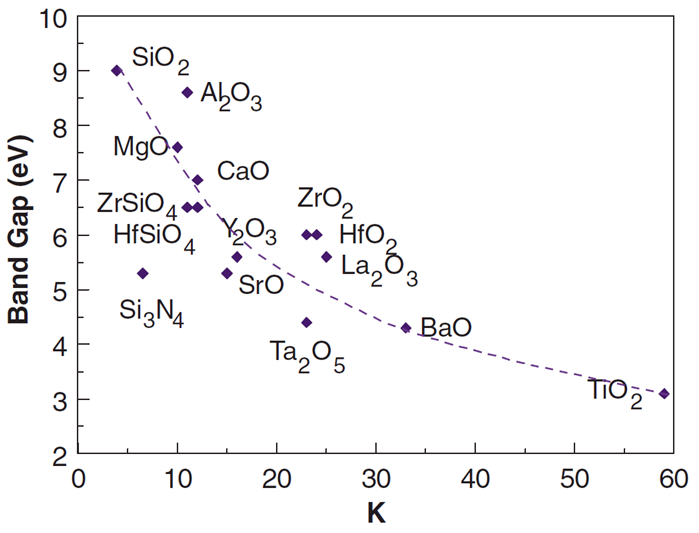
\includegraphics[width=0.7\textwidth]{chapter_1/bandgapvsk}
\caption{Band gap versus dielectric constant for potential high-k gate dielectrics.}
\label{fg:bandgapvsk}
\end{figure}

To demonstrate this point, it is useful to plot the dielectric constant versus band gap (Figure \ref{fg:bandgapvsk}) \cite{Robertson2008}. Figure \ref{fg:bandgapvsk} reveals a roughly inverse dependence on $\varepsilon_{r}$. Assuming that the band gaps align symmetrically with respect to silicon, this means that oxides with larger dielectric constants will likely have a smaller barrier height and are susceptible to leakage currents by Schottky emission. This suggests that dielectrics such as TiO$_{2}$ \cite{Kim2004}, BaTiO$_{3}$ \cite{Arlt1985}, and BaSrTiO3 \cite{Horikawa1993, Hilton1996} may not be suitable alternatives, even though they exhibit very high dielectric constants. In general the conduction band offset is much smaller than the valence band offset, so it is more instructive to plot the dielectric constant as a function of conduction and valence band offsets (Figure \ref{bandoffsetvsk}) \cite{Robertson2008}. Ideally, a band offset of at least 1 eV is desirable. In Figure \ref{bandoffsetvsk} we see that La based group III oxides exhibit a good balance of both high dielectric constant and band offset. Indeed, materials such as LaAlO$_{3}$ \cite{Edge2006} and LaLuO$_{3}$ \cite{Liu2011} show promise as potential high-k gate dielectrics. 

\begin{figure}
\centering
\noindent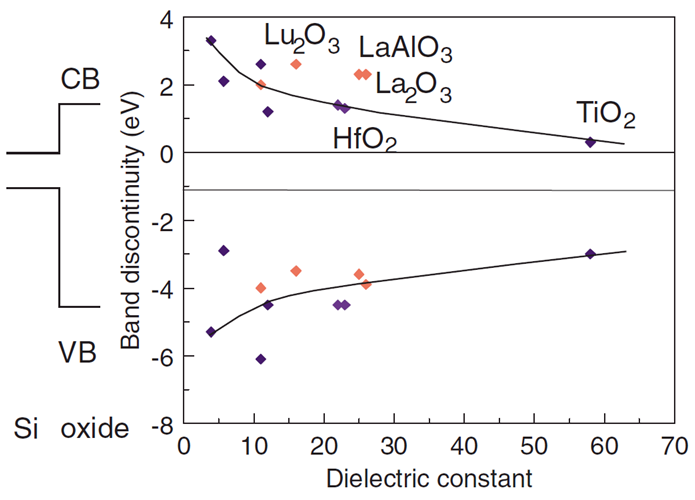
\includegraphics[width=0.7\textwidth]{chapter_1/bandoffsetvsk}
\caption{Measured band offsets of oxides on Si against dielectric constant for candidate gate oxides. Group III oxides are shown in red, HfO$_{2}$ and ZrO$_{2}$ in blue. From Reference \cite{Robertson2008}.}
\label{bandoffsetvsk}
\end{figure}

Other critical factors include interface quality and the thermodynamic and kinetic stability of the oxide in contact with the channel material and the gate electrode. Many potential candidates for gate oxides such as Ta$_{2}$O$_{5}$ and TiO$_{2}$ were initially adopted from DRAM technology \cite{Chaneliere1998,Kingon2000}; however, many turned out to be incompatible as gate oxides due to thermodynamic incompatibility with Si \cite{Hubbard1996a, Schlom2002}. Achieving a good interface and minimizing the defect densities at the oxide-semiconductor interface is also of paramount concern to abate deleterious effects such as charge trapping, which can decrease the carrier mobility in the channel and also cause Fermi level pinning.

\section{Amorphous transition metal-oxide dielectrics}

In the search for a suitable replacement to SiO$_{2}$, one consideration is whether to use an amorphous or crystalline material for the gate oxide. The advantage of amorphous materials is the lack of grain boundaries found in polycrystalline materials, which can act as sites for leakage currents to flow. In addition, the applied field will be uniform across the gate because the dielectric constant does not change with crystal orientation of the dielectric. Note, epitaxial growth of single crystalline oxides can also circumvent the problem of grain boundaries and is currently an area of active research \cite{dai2003}.

The challenge with amorphous materials is that many of the potential high-k gate oxides, such as HfO$_{2}$ and ZrO$_{2}$, crystallize at temperatures required to activate implanted dopants in the channel ($\sim$1000 \textdegree C). Crystallization of the oxide can be suppressed by doping silicates, but this comes at the cost of a lowered dielectric constant \cite{VanDover2003}. A surprising result showing an enhanced dielectric constant for zirconium and hafnium silicates at low SiO$_{2}$ concentrations \cite{Wilk2000, Wilk2000a}, demonstrated the possibility of evading the low-k problem. The result also initiated a slew of experimental and computational attempts to explain the anomalous effect, as it is a peculiar result in amorphous systems. Ultimately, the enhanced dielectric constants were not consistently reproducible \cite{Rignanese2002, Pignedoli2007}, nonetheless it remains to be an interesting theoretical and computational problem. In the following section we provide efforts to understand this anomalous dielectric phenomena in amorphous Hf-Si-O and Zr-Si-O.

\subsection{Dielectric anomalies in amorphous Hf-Si-O and Zr-Si-O dielectrics}

In 2007, Intel announced the introduction of their new transistor incorporating a HfO$_{2}$ $\emph{based}$ gate oxide and a metal gate electrode \cite{Mistry2007}. Work leading up to this involved countless attempts to screen various oxides. From the start a prime candidate was transition metal silicates. The rationale behind the silicates was to compromise a ``high" dielectric constant oxide ($\varepsilon_{r} \sim 22$ for HfO$_{2}$) in exchange for interface quality by doping SiO$_{2}$. Initial results for Hf-Si-O and Zr-Si-O were very promising; the oxides did not react in direct contact with Si up to at least 1050 \textdegree C, leakage currents were less than $\sim$10$^{-6}$ A/cm$^{-2}$ with high breakdown fields on the order of 10 MV/cm \cite{Wilk2000a}. There was evidence that silicates with higher concentrations of transition metal oxide were susceptible to crystallization at lower temperatures  ($<$1000 \textdegree C) \cite{Neumayer2001}, but the addition of nitrogen in the metal silicate was shown to improve thermal stability of the material \cite{Visokay2002}.

The surprising feature is arguably the unexpected enhancement in the dielectric constant. Referring to the original work by Wilk \cite{Wilk2000a}, a simple calculation reveals that the expected value for $\varepsilon_{r}$ with x $\sim$ 17 at.\% Hf in Hf$_{x}$Si$_{1-x}$O$_{2}$ (again, assuming $\varepsilon_{r} \sim 22$ for HfO$_{2}$ and $\varepsilon_{r} \sim 3.9 $ for SiO$_{2}$) is $\sim7$. The authors however report a value of $\varepsilon_{r}$ $\sim$ 11, which is about a 60\% increase from the expected value based on a weighted mean of the metal oxide concentrations. A similar effect is observed for zirconium silicates, denoting their chemical similarities.  

Dielectric enhancement is not unheard of, especially in crystalline form. For example, work by Cava showed that substitution of \ce{TiO2} in \ce{Ta2O5} stabilizes the H' monoclinic phase resulting in a near four-fold increase in the dielectric constant \cite{Cava1995}. A similar approach can be taken for Hf and Zr based oxides, where a high temperature phase (tetragonal or cubic) can be stabilized at room temperature to increase the dielectric constant \cite{Chalker2008a, Fischer2008b, Park2006}. A perfect demonstration of this is the stabilization of tetragonal \ce{HfO2} by substitution of 5 atomic percent \ce{SiO2} followed by a high temperature anneal. Here, the authors report a maximum $\kappa$ value of 27, versus an amorphous value of $\kappa \sim 20 $ \cite{Tomida2006}.

The relationship between the dielectric constant and structure is more tenuous. This of course is not to say that it is impossible to form a relationship between the two, and several experimental and theoretical developments are available on this front for hafnium and zirconium silicates. Initial studies utilizing Fourier Transform Infrared Spectroscopy (FTIR) suggested that the enhancement was due to four-fold coordinated Zr-O bonds \cite{Lucovsky2000}. In contrast, cluster simulations performed by Kurtz and Devine revealed the energetic stability of six-coordinated Zr over four \cite{Kurtz2001}. A six-coordinated Zr cluster would infer a higher local network density, a smaller molar volume, and thus a higher dielectric constant according to the Clausius-Mossotti relation \cite{Kurtz2001}. Calculations by Rigananese et al. related the dielectric constant of Zr-Si-O to local structural units \cite{Rignanese2002}. A modest enhancement of $\epsilon_{r}$ was attributed to ZrO$_{6}$ octahedra, but was not sufficient to account for the large reported enhancement in $\varepsilon_{r}$. Recent large-scale \textit{ab initio} simulations suggest that the inconsistent data for $\varepsilon_{r} (x)$ in amorphous $\textnormal{Zr}_{x}\textnormal{Si}_{1-x}\textnormal{O}_{2}$ and $\textnormal{Hf}_{x}\textnormal{Si}_{1-x}\textnormal{O}_{2}$ is due to variability in local structure associated with the variety of coordination numbers accommodated by the transition metal \cite{Pignedoli2007}.  In that work it was also found that a correlation between $\varepsilon_{r}$ and density could not be established, refuting earlier models for dielectric enhancement based solely on changes in density \cite{Kurtz2001,Devine2001}.

The nontrivial dependence of the dielectric constant of Hf(Zr)-Si-O on local structure clearly indicates a wealth of scientific knowledge that can be gained from studying complex amorphous materials. Next, we present a more recent discovery of a tantalum based amorphous oxide exhibiting anomalous dielectric properties similar to those observed in the Hf(Zr)-Si-O system. These results lead us to believe that this type of behavior is not entirely unique and that there are other amorphous systems which can exhibit unusual properties.

\subsection{Tantalum based amorphous materials and anomalous behavior in Ta-Ge-O}

Tantalum pentoxide is a dielectric material that is used in a variety of technological applications including DRAM memory, antireflective coatings, and the more nascent non-volatile memories \cite{Chaneliere1998, Banno2010}. Structurally, the material is quite complex, with the existence of many polymorphic structures. This is partly due to \ce{Ta}'s large coordination number which can range from six to as large as eight oxygen atoms \cite{Fukumoto1997, Liu2007b}.  Because of this complex structural morphology, it is of great computational and experimental interest \cite{Kimura1995a,Andreoni2010, Bassiri2011, Lee2013}.
\begin{figure}[ht]
\centering
\noindent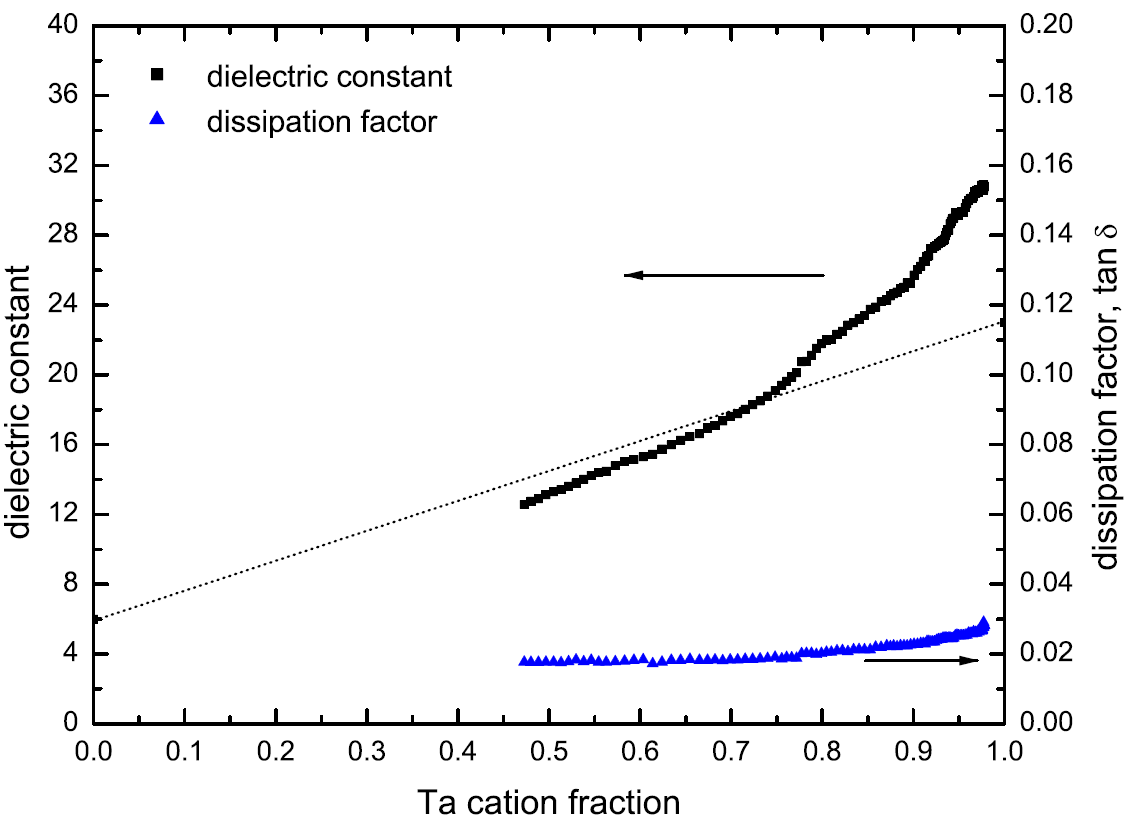
\includegraphics[width=0.7\textwidth]{chapter_1/tageox}
\caption{The variation in dielectric constant (black squares) and dissipation factor (tan d, blue triangles) of Ta$_{x}$Ge$_{1-x}$O$_{y}$ as a function of Ta cation fraction measured at 10 kHz. The dotted line represents the linear interpolation between endmember values. The uncertainty in $\varepsilon_{r}$ is estimated to be $\pm$ 5$\%$, dominated by uncertainty in the ellipsometrically determined thickness. From Reference \cite{Naoi2012}.}
\label{tageox}
\end{figure}

It was recently reported that mixed amorphous tantalum germanium oxide exhibits a dielectric constant, $\varepsilon_{r}$ as much as 40\% higher than that of pure tantalum oxide (Figure \ref{tageox}) \cite{Naoi2012}. Moreover, the dielectric constant exceeds the value of both pure \ce{Ta2O5} and \ce{GeO2}. This was not the case for the Hf(Zr) silicates, in which the dielectric constant only exceeded the value of the lower endmember \ce{SiO2}. Currently there is no coherent rationale which explains this behavior. Through this dissertation we wish to study this material system further in order to understand the underlying mechanisms which give rise to this phenomenon.

\section{Alternative computing and memory architectures: Motivation to study thin film complex amorphous oxides}

It is clear that sooner or later Moore's law scaling will come to an end or need to be completely redefined due to physical limitations or simply becoming too impractical to pursue. In anticipation of this impending limitation, different avenues are already being explored. These include, but are not limited to, advancement in 3D transistors \cite{Hisamoto2000}, quantum computing \cite{Devoret2013}, and neuromorphic computing \cite{Pershin2012}. Similar trends are being pursued in memory storage architectures, which emphasize non-volatile forms of memory \cite{Meijer2008}.

Memory devices expectedly stress different requirements in comparison to logic devices. These are things such as read/write (R/W) times, retention time, number of cycles the memory can endure, energy required to flip the bit, and the maximum achievable memory density. Current R/W times for Hard disk drives (HDDs) are on the order of several milliseconds (Table \ref{table:memory}). Solid state drives based on Flash(NAND) memory improve R/W times by an order of magnitude or two, but still suffer from low endurance (10$^{4}$ cycles). On the other hand, the switching speeds of DRAM capacitors are extremely fast---on the scale of tens of nanoseconds---in addition to exhibiting cycle endurances greater than 10$^{16}$. The clear drawback however, is the ephemeral nature of the memory (retention time $<<$ seconds), since DRAM is not designed for long term memory storage. Comparisons of HDD/Flash memory versus DRAM illustrate the historical trend for memory devices to either sacrifice R/W speeds for retention time or retention time for R/W speeds. Emerging memory technologies such as phase change memory (PCM) and spin torque transfer random access memory (STTRAM) attempt to eliminate the need for this trade-off.

\begin{table}
\centering
\scriptsize
\begin{tabular}{llllllll}
\toprule
& \textbf{Memristor} & \textbf{PCM} & \textbf{STTRAM} & \textbf{SRAM} & \textbf{DRAM} & \textbf{Flash(NAND)} & \textbf{HDD}\\
\midrule
&&\multicolumn{2}{c}{\textbf{Prototype}}& \multicolumn{4}{c}{\textbf{Commercialized technologies}} \\
\cmidrule(lr){3-4} \cmidrule(lr){5-8} 
Reciprocal density (F$^{2}$)  & $<$ 4 & 4-16 & 20-60 & 140 & 6-12 & 1-4 & 2/3 \\
Energy per bit (pJ) & 0.1-3 & 2-25 & 0.1-2.5 & 0.0005 & 0.005 & 0.00002 & 1-10$\times$10$^{9}$  \\
Read time (ns) &  $<$10 & 10-50 & 10-35 & 0.1-0.3 & 10 & 100,000 & 5-8$\times$10$^{6}$\\
Write time (ns) & $\sim$10 & 50-500 & 10-90 & 0.1-0.3 & 10 & 100,000 & 5-8$\times$10$^{6}$ \\
Retention time & years & years & years & As long as & $<<$ second & years & years \\
&&&&voltage &&&\\
&&&&applied&&&\\
Endurance (cycles) &10$^{12}$&10$^{9}$&10$^{15}$&$>$10$^{16}$&$>$10$^{16}$&10$^{4}$&10$^{4}$\\
\bottomrule
\end{tabular}
\caption{Comparison of current memory storage technologies. PCM, phase change memory; STTRAM, spin torque transfer random access memory; SRAM, static RAM, DRAM, dynamic RAM; HDD, hard disk drive. Taken from Reference \cite{Yang2013}.}
\label{table:memory}
\end{table}

On this front, electrical switches that utilize resistance change to store and perform logic operations (e.g. memristors) are most promising \cite{Yang2013}. The concept of switching and memory phenomena involving the differential change in materials resistance has been known for some time \cite{Dearnaley1970}. But recent improvements in the ability to probe materials at the nanoscale have facilitated the observation of microscopic changes in the material with switching. One can also draw from the vast knowledge of device processing accumulated over the years to scale devices down to improve memory density. The challenge now, is to gain a deeper understanding of the switching phenomena and relate the structural changes that occur with the electrical properties of the material in order to design suitable materials. 

Many resistive materials which display switching behavior start amorphous (mixed amorphous/polycrystalline in the work by Kwon et al.) \cite{Yao2010a, Kwon2010a, Lee2011a}, which is equivalent to a ``0".  The material is switched to the ``on" state, equivalent to a ``1," when a conductive crystalline pathway forms between the electrodes. The exact mechanism for the switching behavior is still under debate \cite{Yang2013}, but an understanding of the amorphous structure of amorphous oxides can provide insight into the behavior of such devices. Furthermore, current resistive materials often utilize binary oxides, and thus the resistive behavior of more complex compositions is not very well understood. To characterize the resistive behavior of complex amorphous oxides, multi-component sputtering may prove to be useful. 

\section{Deposition technique: off-axis sputtering for multi-composition research}

The majority of thin film samples in this work were deposited using RF magnetron sputtering. When considering thin film deposition techniques for creating complex amorphous oxides, sputtering provides several advantages over other deposition techniques which are more commonly found in large scale industrial fabs, namely chemical vapor deposition (CVD) and its close cousin, atomic layer deposition (ALD). CVD methods depend on the thermodynamic reactions between volatile precursors. Therefore, film stoichiometry is strongly predicated on the capacity to control the reaction between precursors using various annealing and gas transport processes. This makes CVD type methods suitable for tightly controlling the stoichiometry of uniform films, but unfit for combinatorial depositions that require depositing many compositions in one run. 

Sputtering, in contrast, involves the volatilization of pure metal or ceramic compounds using a plasma, allowing for the deposition of high purity films. When metal targets are used, high purity oxygen is introduced into the chamber to oxidize the volatilized metals. Film stoichiometry can be readily varied across a film in a single run by depositing composition spreads \cite{VanDover2004a}. This is achieved in our lab by orienting the sputtering guns in an oblique configuration, as shown in Figure \ref{fenris}.

\begin{figure}
\centering
\noindent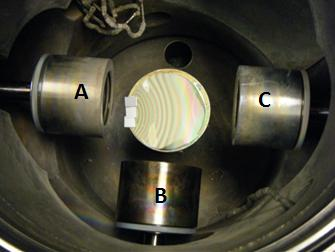
\includegraphics[width=0.7\textwidth]{chapter_1/fenris}
\caption{Top down view inside the sputtering chamber that is used in this work. Three magnetron sputtering guns are in the 90 degree off-axis configuration with respect to the substrate. Sputtering in this configuration results in a natural thickness gradient across the substrate. Guns A, B, and C can be energized simultaneously to create a composition spread.}
\label{fenris}
\end{figure}

When the targets are sputtered in this configuration a natural thickness gradient is obtained across the substrate. Due to the formation of a natural thickness gradient, sputtering from two or more targets simultaneously will also result in a natural composition gradient. The added bonus here is that the sputtered constituents are intimately intermixed, i.e. the atoms form a true atomic scale amorphous mixture. To achieve a similar effect using ALD would be cumbersome since it is a technique that involves layer by layer growth. Also in comparison to discrete combinatorial methods \cite{Xiang1995} the composition resolution of continuous composition methods is much finer, on the order of $\sim$ 0.1 mol\% \cite{VanDover2004a}.

The disadvantage of sputtering is that the sputtering can introduce defects and inclusions in the thin film. Not surprisingly the most common inclusion is Ar for sputtering \cite{Cuomo1977}. There is also the effect of introducing substantial film stress in the film if the substrates are biased during the deposition \cite{Kim1998}. Nonetheless, applying a substrate bias is a necessary process during off-axis deposition to preclude the formation of columnar voids \cite{Barron2009}. Finally, because sputtering is a line of sight deposition technique, it is not suitable for depositions that require high conformity to the surface topology of the device. Ultimately, the utility of the materials discovered and evaluated using the composition spread methods needs to be compatible with deposition techniques used in industry. 

     
% chapter 2
\chapter{Materials Preparation and Analysis}

In this chapter we discuss methods used to prepare and analyze the thin film oxides as well as provide a short review on the theory of dielectrics. 

\section{The dielectric properties of materials}
\subsection{Insulating materials and charge}

Capacitors come in various shapes and sizes, the simplest configuration being the parallel plate capacitor (PPC). The PPC is comprised of an insulating material that is sandwiched between two conducting terminals (Figure \ref{fig:PPC}a). If we consider a PPC in a vacuum with only space between the two terminals connected to a battery, the capacitance between the terminals is:
\begin{equation} \label{eq:capfreespace}
C_{o} = \frac{Q_{o}}{V}.
\end{equation}
Here, $C_{o}$ is the capacitance of the parallel plate capacitor in free space, $Q_{o}$ is the charge on the terminals, and $V$ is the voltage that is applied between the terminals. Now, if we slide an insulating material between the two terminals as shown in Figure \ref{fig:PPC}b,
\begin{figure}[t]
	\centering
	\begin{subfigure}[b]{\linewidth}\centering
	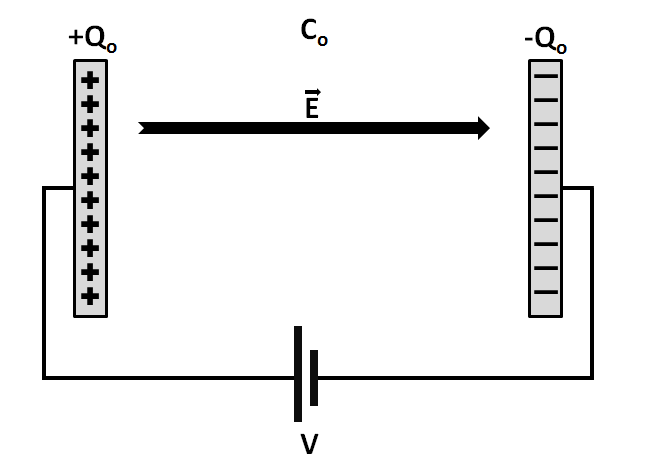
\includegraphics[width=.7\linewidth]{chapter_2/cap1}
	\caption{}\label{fig:sub1}
	\end{subfigure}\
	\begin{subfigure}[b]{\linewidth}\centering
	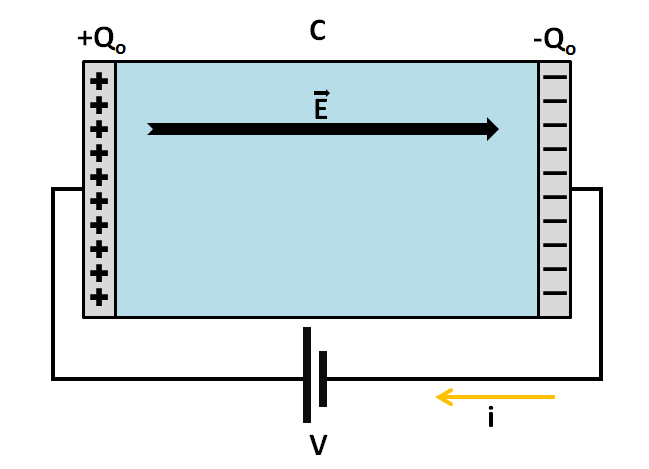
\includegraphics[width=.7\linewidth]{chapter_2/cap2}
	\caption{}\label{fig:sub2}
	\end{subfigure}
	\caption{(a) Parallel plate capacitor in a vacuum connected to a battery with voltage V and capacitance C$_{o}$. (b) The capacitance changes from C$_{o}$ to C when an insulating material is placed between the terminals. }
	\label{fig:PPC}
\end{figure}
current would immediately flow through the external circuit resulting in an increased amount of separated charge. The new charge at the two terminals is now $Q$ such that the capacitance changes to $C$, so equation \ref{eq:capfreespace} is slightly modified to
\begin{equation} \label{eq:capreal}
C = \frac{Q}{V}.
\end{equation}
The ratio between the initial and final charge stored in the capacitor is the relative dielectric constant $\varepsilon_{r}$ (also written as $\kappa$ or $k$) 
\begin{equation}
\frac{Q}{Q_{o}} = \varepsilon_{r}
\end{equation}
and alternatively, the ratio between the two capacitances
\begin{equation}\label{eq:cap0}
\frac{C}{C_{o}}=\varepsilon_{r}.
\end{equation}
This simple example shows that dielectrics are essentially charge storage devices and that the dielectric constant is a  parameterization of how effectively a material is able to store charge. Due to its simplicity, many modern electronics exploit the parallel plate configuration. One thing to note is that due to finite size effects the field lines that go from one side of the terminal to the other, especially on the periphery of the terminals, are not perfectly straight lines (Figure \ref{fig:cap3}).

\begin{figure}[t]
	\centering
	\begin{subfigure}[b]{\linewidth}\centering
	\centering
	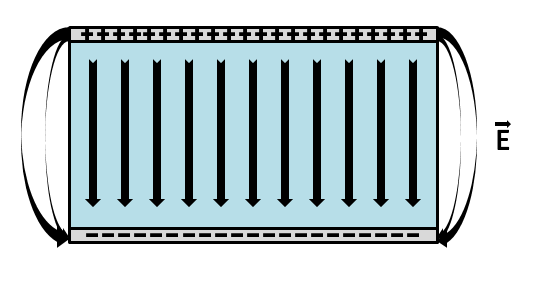
\includegraphics[width=0.7\linewidth]{chapter_2/cap3}
	\caption{}\label{fig:cap3}
	\end{subfigure}
	\begin{subfigure}[b]{\linewidth}\centering
	\centering
	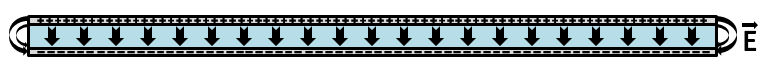
\includegraphics[width=0.7\linewidth]{chapter_2/cap4}
	\caption{}\label{fig:cap4}
\end{subfigure}

\caption{The contribution of the fringing field to the total electric field changes with the aspect ratio of the capacitor. Thin film capacitors have a large aspect ratio so the contribution of the fringing field is minimal.}
\end{figure}

Field lines at the outer edges of the capacitor---so-called fringing fields---are not entirely contained between the plates. For our devices we assume that these fringing fields do not contribute significantly to the electrical measurement owing to the large aspect ratio between the thickness of the insulating film (d)---ranging from $\sim$10 to several 100 nanometers---and the width of the capacitors (w) (several hundred microns) in our devices, which allows us to greatly simplify the integral equation of Gauss's law. For a capacitor with no dielectric, 
\begin{equation}\label{eq:gauss_law}
\oiint_{S}\vec{\textbf{E}}\cdot d\vec{\textbf{A}} = E_{o}A= \frac{Q_{o}}{\varepsilon_{o}}
\end{equation} 
in which $E_{o}$ is the electric field between the two plates, $A$ is the area of the capacitor, and $\varepsilon_{o}$ is the permittivity of free space. Combining with equation \ref{eq:capfreespace}, rearranging, and from the fact that $E_{o} = Vd$, we can relate the capacitance to the applied electric field,
\begin{equation}\label{eq:cap1}
\frac{\varepsilon_{o}AE_{o}}{V} = \frac{\varepsilon_{o}A}{d} =C_{o}.
\end{equation}
Recall, that for a capacitor with an insulating material the capacitance is larger by a constant factor $\varepsilon_{r}$
\begin{equation}
\label{eq:cap2}
C = \frac{\varepsilon_{o} \varepsilon_{r} A}{d}.
\end{equation}
Equation \ref{eq:cap2} illustrates the dependence of capacitance on geometry, namely capacitance area and distance between plates, and intrinsic electronic properties through $\varepsilon_{r}$. Our study focuses on the composition dependence of $\varepsilon_{r}$ for amorphous dielectric oxides. Thus, we introduce the concept of dielectric polarization to describe their intrinsic properties. 

\subsection{Polarization}

As we saw earlier, inserting a dielectric between two electrical terminals changes the capacitance between the two terminals. This is a result of the atoms in the dielectric spontaneously polarizing in order to align with the electric field. \textit{Classically}, the spontaneous polarization of the atoms can be represented as a chain of positive and negative point charges that connect head to tail (Figure \ref{cap5}).
\begin{figure}
\centering
\noindent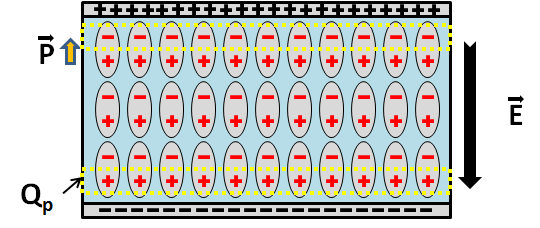
\includegraphics[width=0.7\linewidth]{chapter_2/cap5}
\caption{Application of an external electric field causes the atoms in the material to polarize along the direction of the applied field. Consequently, a surface polarization charge $Q_{p}$ forms at the interface between the electrode and the dielectric.}
\label{cap5}
\end{figure}
The polarization of the atoms within the material in turn causes the surface of the dielectric to polarize, forming a \textit{surface polarization} charge $Q_{p}$. We can consider the surface polarization charge to be a single dipole moment $p$ across the dielectric. We define polarization to be the total dipole moment per volume, which is equivalently represented as a \textit{surface polarization charge density} $\sigma_{p}$
\begin{equation}\label{eq:polarization}
P = \frac{p}{V} = \frac{Q_{d}d}{Ad} = \frac{Q_{p}}{A} = \sigma_{p}.
\end{equation}
To compensate for the new charge $Q_{p}$ that has formed on the surface of the dielectric, current flows through the external circuit (recall Figure \ref{fig:PPC}b). As a result, the free surface charge $Q_{o}$ becomes $Q$. The total charge on the plates can be  expressed as
\begin{equation}\label{eq:totalcharge}
Q = Q_{o} + Q_{p}.
\end{equation}

If we divide equation \ref{eq:totalcharge} by the area of the capacitor $A$, we can rewrite equation \ref{eq:totalcharge} in terms of charge densities $\sigma$
\begin{equation}\label{eq:charged}
\sigma = \sigma_{o}+\sigma_{p}.
\end{equation}
From equation \ref{eq:polarization} we know that $\sigma_{p}$ is the surface polarization density and $\sigma_{o}$ is just the \textit{free surface charge density}. The free surface charge density can be written in terms of the electric field, $E$ by rearranging equation \ref{eq:gauss_law}
\begin{equation}\label{eq:charge2}
\sigma = \varepsilon_{o}E + \sigma_{p}.
\end{equation}
Substituting $P$ for $\sigma_{p}$ and since $P = \chi_{e}\varepsilon_{o}E$ we get 
\begin{equation}\label{eq:charge3}
\frac{\sigma}{E } = \varepsilon_{o}(1+\chi_{e})
\end{equation}
where $\chi_{e}$ is the electric susceptibility. Finally, we can relate equation \ref{eq:charge3} back to capacitance 
\begin{equation}\label{eq:charge4}
\frac{\sigma}{E } = \frac{Q}{AE} = \frac{Cd}{A} = \varepsilon_{o}(1+\chi_{e})
\end{equation}
\begin{equation}\label{eq:charge5}
C = \frac{\varepsilon_{o}(1+\chi_{e})A}{d} =  \frac{\varepsilon_{o} \varepsilon_{r} A}{d} 
\end{equation}
so $(1+\chi_{e})= \varepsilon_{r}$.

The simple relation between relative permittivity, capacitance, and susceptibility suggests that measuring the capacitance of the PPC reveals information about the polarization of atoms. For instance, if a polarizable medium did not exist between the conducting terminals (vacuum) $\chi_{e} =  0$, we would be left with equation \ref{eq:cap1}. On the other hand, when an polarizable (e.g. insulator) material was present $\chi_{e} > 0$, the capacitance would be greater by a constant $\varepsilon_{r}$.

\subsection{Local field, Clausius-Mossotti, and polarizability}

We have made the point that macroscopic dielectric properties have microscopic origins. We develop this concept further by establishing a connection between the dielectric constant and polarizability of the atom. 

As mentioned earlier, when an electric field $\textbf{E}_{o}$ is applied to a dielectric the atoms polarize to align with the field. However, the electric field felt by each atom---the ``local field" ($\textbf{E}_{\text{loc}}$)---is in fact different from the externally applied field, $\textbf{E}_{o}$. We calculate the local field by cutting out a hypothetical cavity in the material centered at $i$, and removing atom $i$ (the atom cannot produce its own field) as shown in Figure \ref{depfield}.

\begin{figure}
\centering
\noindent
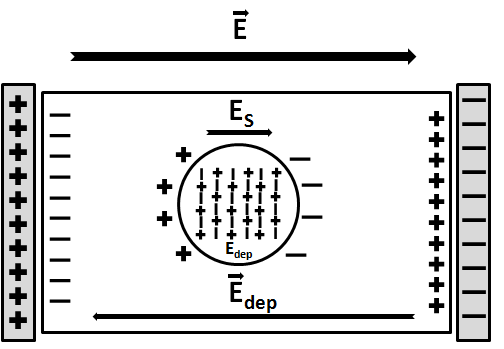
\includegraphics[width=0.7\textwidth]{chapter_2/depfield}
\caption{To calculate the local field felt by the atom inside the material we create a hypothetical cavity in the material, creating a uniformly polarized sphere. The local field is determined by summing all the contributions to the local field.}
\label{depfield}
\end{figure}

The local field at atom $i$ is determined by summing the different contributions to the local field. The contributions from outside of the cavity $\textbf{E}(\textbf{r})$ equal the difference between the applied field and the depolarization field $\textbf{E} = \textbf{E}_{o} - \textbf{E}_{dep}$. Within the cavity we have contributions from $\textbf{E}_{\text{sphere}}(\textbf{r})$, which is the macroscopic field inside a uniformly polarized sphere, and local dipolar contributions of the atoms within the cavity, $\textbf{E}_{\text{dipolar}}(\textbf{r})$. We write $\textbf{E}_{\text{loc}}(\textbf{r})$ as
\begin{equation}\label{eq:local}
\textbf{E}_{\text{loc}}(\textbf{r}) = \textbf{E}(\textbf{r}) + \textbf{E}_{\text{sphere}}(\textbf{r}) + \textbf{E}_{\text{dipolar}}(\textbf{r}).
\end{equation}

From electrostatics, we know that $\textbf{E}_{\text{sphere}}(\textbf{r})$ is $4\pi\textbf{P}(\textbf{r})/3$, where $\textbf{P}(\textbf{r})$ is the polarization density defined as \textbf{P} $(\textbf{r}) = \textbf{p}(\textbf{r})/\textit{v}$, that is, polarization per unit volume. Equation \ref{eq:local} is further simplified for high symmetry materials. For these materials, e.g. cubic and amorphous materials, we assume that dipolar term, $\textbf{E}_{\text{dipolar}}(\textbf{r})$ vanishes. Now, the local field is 
\begin{equation}\label{eq:local2}
\textbf{E}_{\text{loc}}(\textbf{r}) = \textbf{E}(\textbf{r}) + \frac{4\pi\textbf{P}(\textbf{r})}{3}.
\end{equation}

The following,
\begin{equation}\label{eq:disp}
\textbf{D}(\textbf{r}) = \varepsilon\textbf{E}(\textbf{r})
\end{equation}
relates the electric displacement $\textbf{D}(\textbf{r})$ to the dielectric constant $\varepsilon$. Using Equations \ref{eq:local2} and \ref{eq:disp}, we can express $\textbf{P}(\textbf{r})$ in terms of $\textbf{E}(\textbf{r})$
\begin{equation}\label{eq:disp2}
\textbf{P}(\textbf{r}) = \frac{\varepsilon - 1}{4\pi}\textbf{E}(\textbf{r}).
\end{equation}
Combining Equation \ref{eq:local2} and \ref{eq:disp2} eliminates $\textbf{P}(\textbf{r})$ and becomes an equation that links the local electric field $\textbf{E}_{\text{loc}}(\textbf{r})$ to measurable quantities
\begin{equation}
\textbf{E}^{\text{loc}}(\textbf{r}) = \frac{\varepsilon + 2}{3}\textbf{E}(\textbf{r}).
\label{eq:eloc}
\end{equation}
Polarization of the atom is related to the polarizability and local field by $\textbf{p}(\textbf{r}) = \alpha\textbf{E}_{\text{loc}}(\textbf{r})$. Recalling that $\textbf{P}(\textbf{r}) = \textbf{p}(\textbf{r})/v$, we can use Equation \ref{eq:disp2} and \ref{eq:eloc} to obtain the Claussius-Mossotti equation 
\begin{equation}
\frac{\varepsilon - 1}{\varepsilon + 2} = \frac{4\pi\alpha}{3v}.
\label{eq:CM}
\end{equation}
The Claussius-Mossotti (CM) equation is a much used equation that relates a local property---polarizability, $\alpha$---to a macroscopic property, the dielectric constant. 

In actuality, the situation is a bit more subtle. A more thorough investigation of the phenomena of polarization reveals the ambiguity of assigning individual dipole moments to atoms and the choice of a proper primitive cell, known as the polarization ambiguity. There have recently been several theoretical developments that have led to sophisticated methods allowing researchers to calculate the spontaneous polarization of periodic solids \cite{Spaldin2012}. However, the aperiodicity of amorphous materials still poses a theoretical and computational challenge due to the lack of long range ordering. In this study, we merely rely on the CM equation as a way to experimentally extract trends in how polarizability (a local property) changes as a function of concentration. 

\subsection{Frequency dependence}

The process of polarization is an inherently frequency dependent process. Different polarizability mechanisms are accessible at different frequencies and give rise to the dispersive behavior of the dielectric constant (Figure \ref{fig:polardisp}).

\begin{figure}[ht]
\centering
\noindent
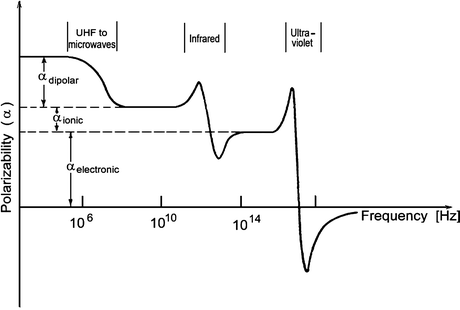
\includegraphics[width=0.7\linewidth]{chapter_2/polarizabilitydispersion}
\caption{Dispersion relation of polarizability as a function of frequency. Figure taken from reference \cite{Subhadra2011}.}
\label{fig:polardisp}
\end{figure}

For dielectric materials that are presented in this study, the components that contribute to the dielectric constant are mainly electronic ($\alpha_{electronic}$) and ionic ($\alpha_{ionic}$) polarizabilities. The total polarizability can be described as a linear combination of these mechanisms
\begin{equation}\label{eq:totalpolarziation}
\alpha_{total} = \alpha_{electronic} + \alpha_{ionic}
\end{equation}
and are both roughly active up to infrared frequencies ($\sim10^{12}$ Hz) (Figure \ref{fig:polardisp}).

Accurate modeling of polarizabilities requires detailed theoretical considerations, but we can describe to first order their behavior using crude models. Using these crude models the electronic and ionic polarizabilities are written as

\begin{equation}
\alpha_{electronic} = \frac{Z_{i}e^{2}}{m (\omega_{o}^{2} - \omega^{2})}
\qquad
\alpha_{ionic} = \frac{e^{2}}{M (\bar{\omega}^{2} - \omega^{2})}
\end{equation}
where $Z$ is the atomic number, $e$ is the electric charge, $m$($M$) is the mass of the electron(ions), $\bar{\omega}$ is the resonance frequency of the crystal, $\omega_{o}$ is the frequency of the electronic shell, and $\omega$ is the driving frequency of oscillation. It is not surprising that these two equations are similar in form since they are both theoretically based on frequency dependent displacement of mass (similar equations of motion). Another point is that the resonance frequency $\bar{\omega}$ of the lattice is considerably smaller in comparison to the frequency of the electronic shell, $\omega_{o}$. This gives rise to the dispersive behavior of $\alpha$ because the rate at which the denominator increases for $\alpha_{ionic}$ is much slower compared to $\alpha_{electronic}$.

According to Equation \ref{eq:CM}, an anomalous change in the dielectric constant would require that either the electronic or ionic term of the polarizability be greatly enhanced, or that there be a substantial decrease in the molecular volume. It is more likely however, that large enhancements are a result of anomalous behavior of the phonons, which is related to $\alpha_{ionic}$. For special classes of materials such as ferroelectrics, the softening of certain modes is an indication of a ferroelectric phase transition \cite{Nuzhnyy2009}. We refer to the Lydanne-Sachs-Teller relation,
\begin{equation}
\frac{\omega_{LO}^{2}}{\omega_{TO}^{2}} = \frac{\varepsilon(\omega = 0)}{\varepsilon(\omega = \infty)}
\end{equation}
to show that at the ferroelectric transition point, the static dielectric constant, $\varepsilon (\omega = 0)$ diverges, implying that  $\omega^{2}_{TO} \rightarrow 0$. The softening of phonon modes can also be observed in non-ferroelectric materials such as quartz. The point here is that since the ionic polarizability of the material is intimately related to the phonons, an enhancement in the dielectric constant would indicate an enhancement in $\alpha_{ionic}$.

At frequencies beyond $\sim10^{12}$ Hz the nucleus of the atom is too sluggish to respond to the alternating electric field and thus, ionic polarization becomes negligible. The total polarization reduces to just the electronic component and the Clausius-Mossotti relation reduces to the Lorentz-Lorenz equation
\begin{equation}\label{eq:LL}
\frac{n^{2}-1}{n^{2}+2} = \frac{4\pi\alpha_{electronic}}{3v}.
\end{equation}
We can obtain the refractive index using optical techniques and use x-rays to determine the molecular volume of the material.

To capture the inherent frequency dependent nature of the dielectric constant in experiment, we write $\varepsilon_{r}$ as a complex function,
\begin{equation}\label{eq:diecomp1}
\varepsilon_{r} = \varepsilon '_{r} - i \varepsilon_{r}''
\end{equation}
where $\varepsilon '_{r}$ and $\varepsilon_{r}''$ are the real and imaginary parts of the dielectric constant, respectively. The real part of the dielectric constant is, $\varepsilon '_{r}$, is the measured relative permittivity in, for example, the capacitance in a PPC. On the other hand, $\varepsilon_{r}''$ represents the energy lost during the polarization process, for instance, by collision with neighboring atoms resulting in energy lost as heat.

We define the loss tangent, $\tan{\delta}$ (also known as the dissipation factor), which equals the ratio between the real and imaginary parts of the dielectric constant
\begin{equation}
\text{tan}\,\delta = \frac{\varepsilon''_{r}}{\varepsilon'_{r}}.
\end{equation}
A high dissipation factor implies that the lossy component of the dielectric constant is large. The lossiness of the dielectric is usually a symptom of poor film quality, i.e. the presence of defect modes and are generally undesirable because they exhibit a significant amount of dispersion in the dielectric constant. Modern devices require high quality control and stability of electronic properties over a large frequency range, so we would like to minimize the frequency dispersion of the oxide. We therefore require films to have a low dissipation factor ($<$0.05).

\section{Synthesis of materials and devices}
\subsection{Capacitor fabrication}

Metal-insulator-metal (MIM) capacitors were fabricated and evaluated combinatorially to explore new amorphous dielectrics as well as to characterize known systems. The advantage of the MIM structure is its simplicity and the flexibility to assess a wide range of technologically relevant metrics. Our studies were mainly concerned with the dielectric properties of oxides and as such, we used the dielectric constant as a figure of merit when evaluating the MIM capacitors. To determine the resistive behavior of resistive memory devices, the MIM can also potentially be adapted to determine the resistive behavior of the material by measuring the I-V curve.

The majority of MIM capacitors were fabricated on 75 mm, 350 $\mu$m thick (100) Si wafers utilizing two deposition methods: electron beam (e-beam) evaporation for the deposition of metal electrodes and rf magnetron sputtering to deposit the oxide films. The general procedure is as follows. Blank Si wafers were first coated with 300 \AA\;Cr adhesion layer using e-beam evaporation. Then without breaking vacuum, a 300 \AA\;Pt base electrode layer was deposited, also using e-beam evaporation. The samples were removed from the evaporator and transferred to the sputtering chamber. Whole wafers were typically used, but in some cases cleaved to smaller pieces in order to accommodate for the size limitations of some measurement apparatuses. The chamber is capable of simultaneously depositing from up to three sputtering targets in the ``off-axis" configuration as shown in Figure \ref{fenris2}.

\begin{figure}[ht]
\centering
\noindent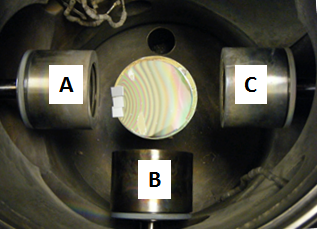
\includegraphics[width=0.6\textwidth]{chapter_2/fenris2}
\caption{Off-axis configuration of the guns enable combinatorial studies of thin film amorphous oxides. Up to three sputtering guns can be energized simultaneously to form a ternary composition. RF biases are applied to the substrate to form a dense film.}
\label{fenris2}
\end{figure}

Here, off-axis means the target face is oriented perpendicular to the sample surface. Deposition from a single target in this configuration results in a natural thickness gradient across the wafer due to the exponential decrease in deposition rate with distance. Thus, when multiple sputtering guns are active a natural composition gradient is obtained. Because of the intimate intermixing of the sputtered constituents, the compositional resolution that can be achieved is typically better than $<$ 0.1 mole-$\%$. Note, the chamber is capable of sputtering in the conventional ``on-axis" configuration as well, where the target face is oriented parallel to the sample surface. This orientation was preferred when single composition films of uniform thickness was required.

Base pressures down to 10$^{-6}$ Torr were achieved by using a turbo molecular pump that is backed by a roughing pump. A gate valve is throttled to control the chamber pressure during deposition. Film thicknesses generally varied from approximately 10 to 300 nm. An rf bias was often applied to the films during off-axis deposition to preclude the formation of voidy films. These voids have been shown to exhibit defect mediated polarization mechanisms that are undesirable for material integration into practical devices \cite{Barron2009}. Once the films were deposited the samples were transferred back to the evaporation chamber. This time, 300 \AA\;Pt dots were deposited onto the sample by evaporation through a shadow mask with 200 $\mu$m diameter holes arranged in a square array with center to center spacing of 500 microns. 

\subsection{Application of e-beam evaporation of metal electrodes and electrode material choices}

E-beam evaporation is a technique that uses high energy electron beams to evaporate source materials in a vacuum. Typically the evaporators are encased in a bell jar, and evacuated to $\sim$ 10\textsuperscript{-7} Torr prior to deposition. A large current is passed through a metal filament causing electrons to boil off thermionically and accelerate towards the source material, which is resting inside a water cooled hearth. The electrons are steered by the magnetic field produced by a solenoid. The force on the electron can be calculated using the Lorentz force equation, $\textbf{F} = q_{e}\textbf{E} + q_{e}\textbf{v} \times \textbf{B}$. The field can also be modulated so that the electron beam rasters across the source material, improving deposition uniformity. The main advantage over thermal evaporation is that e-beam evaporation can be used to evaporate most any material, even highly refractory metals. Although the energy input of the electron beam on the source material far exceeds the strength of the chemical bonds of the material, the overall process is still thermal. Thus the atoms are deposited with energy of $\sim$ 0.2 eV. The fact that it is a line of sight process is also favorable for the use of a shadow mask and minimizing the formation of penumbra caused by insufficient shadowing.  

Some consideration is required when choosing the material that is to be used as electrodes. Because we are measuring the electrical properties of thin film amorphous oxides using MIM structures, we would like to minimize the amount of interfacial oxide formation that would result in inaccurate characterization of the thin film. As an electrode material, platinum is an obvious choice because it is a chemically inert material. However, silicon has a native surface oxide that inhibits the direct deposition of noble metals such as Au and Pt directly onto Si because of their different bonding characteristics. In such a case, a metal that is chemically more reactive needs to be deposited beforehand as an adhesion layer. In this study, a 300 \AA\;layer of Cr was commonly used, but other ``reactive" metals such as Ti would also suffice. A thickness of 300\;\AA\;is more than enough material to yield a continuous layer. 
	
\subsection{Reactive radio frequency magnetron sputtering and the co-sputtering technique}

Sputtering, like e-beam evaporation, is an energy vaporization method, making it suitable for depositing a wide range of materials. However, evaporation is a thermal process, whereas sputtering involves momentum transfer of partially ionized gas particles in the form of a plasma. Conservation of energy and momentum tells us that if two particles are of similar mass, then only a small amount of energy is required to displace the particles from their rest state. For this reason, inert gases such as Ar, Kr, and Xe are suitable choices as impinging particles because of their comparable masses to the target elements. Furthermore, they are generally inexpensive and high in purity. For this study, we used Ar---specifically Ar\textsuperscript{+}---as the impinging gas.

Energy input of ionized gas ions in sputtering usually ranges from 10 to a few 100 eV. Low energy ions can be used for surface modification or densification of films \cite{Coburn1972, Huang2010}, while higher energies are required for sputtering. Dislodged (sputtered) target atoms typically acquire kinetic energies up to several electron volts and undergo various reactions such as colliding with reactive gasses (reactive sputtering), generating secondary electrons before eventually condensing onto the substrate. The final structure and morphology of the thin film ultimately depends on several tunable parameters. 

Structural control can be achieved using various flavors of sputtering. In our study we mainly use rf magnetrons. Rf sputtering is a flexible technique that can be used to deposit from both metals and insulating targets. Sinusoidal power is applied to the driven electrode, with frequency of oscillation typically at 13.56 MHz. Initially during the positive half of the cycle, the electrons respond to the electric field and are drawn to the cathode. However, when the electrode is driven negative, the ions are unable to respond to the sudden change in electric field due to their large size. Thus, the amount of ion current that flows through the target is significantly smaller in comparison to the electron current. Flow of excess electron current is most often impeded by the use of a blocking capacitor. As time progresses the power and the coupling capacitor continues to charge negatively (almost instantaneously). Eventually a steady state is reached and the target is negatively self-biased. Maximum power delivery to the target is accomplished by means of a matching network that works in parallel with the blocking capacitor. 

Use of planar magnetron sputtering guns instead of planar-diode further improves sputtering efficiency. Powerful circular magnets embedded in planar magnetron guns produce magnetic field lines that emanate out into the chamber and curl around back into magnets at the center of the gun. When an electric field is simultaneously applied across the planar cathode, it creates a region where the electric and magnetic fields cross perpendicularly. Electrons in this region travel in a cycloidal pattern and become confined to that region. Consequently, ionization of gas atoms is most efficient there, producing a circular race-track erosion pattern. Magnetron sputtering has the effect of nonuniform erosion patterns across the target surface, but only requires a low working pressure to sputter materials. Therefore the deposition rate is increased due to decreased collisions and lower voltage requirements to sustain the plasma due to the confinement of electrons. 

Most films in this study were sputtered reactively; films were deposited from metal targets in the presence of a working and reactive gas. The gaseous cocktail consisted of Ar as our working gas and O$_{2}$ as the reactive component. Reactive sputtering has several advantages over sputtering directly from a compound (ceramic) target. For one, metal targets can be sputtered at a higher deposition rate compared to ceramic targets and are not as brittle and prone to thermal shock. Higher target purity is also achievable with metal targets so in theory the deposited films should be of higher purity. However, because the target atoms must undergo reactions with the reactive gas to form compounds, in practice one has to consider appropriate partial pressures and gas compositions ratios during deposition to ensure stoichiometric deposition from a metal target. This can be done by controlling the working pressure of the deposition chamber during sputtering, and also by changing the flow rate of the gasses using a mass flow controller.


\section{Characterizing dielectric properties}
\subsection{Capacitance measurements}

Capacitance measurements were performed using a semi-automatic probe station controlled by Labview software, capable of mapping the capacitance and dissipation of an entire 3 inch wafer. Contact to the Pt top electrode was made using a BeCu probe tip, while gold wire was soldered to an exposed portion of the Pt bottom electrode with indium. The probe and gold wire are both connected to a Hewlett Packard 4284A inductance-capacitance-resistance meter (LCR) with a stripped coaxial cable. The LCR meter works by applying AC voltage ($V$) and recording the current ($I$) which is used to calculate the capacitance and dissipation factor based on their phase relation. In this study, the applied AC voltage was on the order of 100 mV.

Both current and voltage are complex quantities and thus can be expressed as complex exponentials with phase lag $\theta$ between the two quantities,   
\begin{equation}\label{eq:I}
V = \vert V\vert e^{j\omega t}
\end{equation}
\begin{equation}\label{eq:V}
I = \vert I\vert e^{j(\omega t + \theta)}.
\end{equation}
In an ideal capacitor the current leads the voltage by $\pi/2$ so any deviation from this value is symptomatic of a non-ideal (real) capacitor. As discussed earlier, the impedance of a real capacitor has contributions from lossy and non-lossy components. Hence, the ratio between the current and voltage is the complex impedance and can be expressed in the following way:
\begin{equation}\label{eq:cap}
\frac{V}{I} = Z = R + jX_{c}.
\end{equation}
Here, $R$ represents the real portion of the impedance (resistance), $X_{c}$ is the imaginary component known as the reactance, and $j$ is the imaginary number $j = \sqrt{-1}$. We can represent the quantity Z as a vector composed of real and imaginary components $R$ and $X_{c}$ as in Figure \ref{fig:compleximpd}.

\begin{figure}[ht]
\centering
\noindent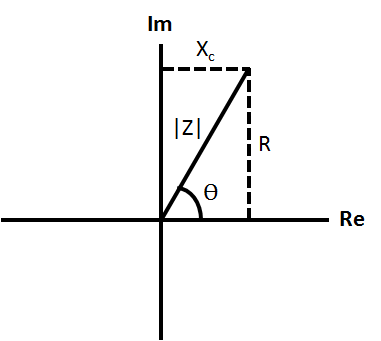
\includegraphics[width=0.5\textwidth]{chapter_2/compleximpedance}
\caption{Complex impedance.}
\label{fig:compleximpd}
\end{figure}

The magnitude of the impedance $\vert Z\vert$ and angle $\theta$ denoting the phase difference between $R$ and $X_{c}$ is,    
\begin{equation}\label{eq:magZ}
\vert Z\vert = \sqrt{R^{2} + X_{c}^2}
\end{equation}
\begin{equation}\label{eq:thetaZ}
\theta = \tan{\left(\frac{X_{c}}{R}\right)}^{-1}
\end{equation}
For mathematical simplicity, it is convenient to write the impedance as admittance $Y$, which is just the inverse of $Z$,
\begin{equation}\label{eq:admit}
\frac{1}{Z} = Y = G + jB_{c}
\end{equation}
such that now $\vert Z \vert$ and $\theta$ are 
\begin{equation}\label{eq:magD}
\vert Z\vert = \sqrt{G^{2} + B_{c}^2}
\end{equation}
\begin{equation}\label{eq:thetaD}
\theta = \tan{\left(\frac{G}{B_{c}}\right)}^{-1}
\end{equation}
in which $G$ is known as the conductance and $B_{c}$ is the susceptance with value $\vert\omega C\vert$. Therefore, the dissipation factor D is, 
\begin{equation}\label{eq:tand}
D = \tan{\delta} =  \tan{\frac{\vert\omega C\vert}{G}}
\end{equation}
and is related to $\theta$ by $\delta = \pi/2 - \theta$. Finally, since we known the film thickness and contact area of the metal electrodes in the MIM capacitors, we can use the measured capacitance to calculate the dielectric constant using equation \ref{eq:cap2}.

\subsection{Optical measurements}

At optical frequencies the atomic nuclei are too sluggish to respond to the alternating electric field, thus only the electronic response contributes significantly to the relative permittivity. The dielectric response at optical frequencies is expressed as the complex refractive index $\tilde{n} = n + ik$, which is a complex quantity written in terms of the absorption coefficient $k$, and $n$, the ratio between the speed of light in a vacuum and the speed of light in a medium. We can determine $n$ and $k$ as well as geometric properties such as film thickness by conducting optical measurements; in our case we use variable angle spectroscopic ellipsometry (VASE). 

Ellipsometry works by shining light onto the surface of the material and measuring the change in polarization of the light after it has interacted with the material. For a single interface, we can quantify the polarization of the light in terms of the Fresnel reflection coefficients ($r_{p}$) and ($r_{s}$), the p and s-polarization components, respectively
\begin{equation}
r^{p}_{12} = \frac{\tilde{N_{2}}\cos{\phi_{1}} - \tilde{N_{1}}\cos{\phi_{2}}}{\tilde{N_{2}}\cos{\phi_{1}} + \tilde{N_{1}}\cos{\phi_{2}}}
\qquad
r^{s}_{12} = \frac{\tilde{N_{1}}\cos{\phi_{1}} - \tilde{N_{2}}\cos{\phi_{2}}}{\tilde{N_{1}}\cos{\phi_{1}} + \tilde{N_{2}}\cos{\phi_{2}}}.
\label{eq:fres}
\end{equation}
In the equation, $\tilde{N_{1}}$ and $\tilde{N_{2}}$ denote the complex refractive index of materials 1 and 2, and $\phi_{1}$ and $\phi_{2}$ are the angle of incidence and transmission from medium 1 to medium 2, respectively. Now, to describe a two interface material the total reflection coefficients for the p and s-polarized components $R_{p}$ and $R_{s}$ can be explicitly written as, 
\begin{equation}
R^{p} = \frac{r^{p}_{12}+r^{p}_{23}e^{-j2\beta}}{1+r^{p}_{12}r^{p}_{23}e^{-j2\beta}}
\qquad
R^{s} = \frac{r^{s}_{12}+r^{s}_{23}e^{-j2\beta}}{1+r^{p}_{12}r^{s}_{23}e^{-j2\beta}}.
\label{eq:refcof}
\end{equation}
The subscripts denote the incident medium and transmitted medium, while $\beta = 2\pi \frac{d}{\lambda}\tilde{N_{2}} \cos{\phi_{2}}$ describes the phase shift of the light that occurs when passing through the various mediums. 

We can combine these quantities in the fundamental equation of ellipsometry
\begin{equation}
\frac{R_{p}}{R_{s}} = \tan{(\psi)}e^{i\Delta}.
\label{ref:ellipsometry}
\end{equation}
The amplitude ratio of reflection, $\tan{(\psi)}$,  and phase shift, $\Delta$, can be measured experimentally, however relevant optical and geometric parameters such as film thickness and refractive index are calculated by fitting to a model. Note, the variability of the angle and the spectroscopic nature of the measurement increases the number of fitted parameters, making the fitting process  more robust. For many optically transparent non-absorbing materials---oxides being one of them---the Cauchy relation provides a simple empirical solution. The Cauchy dispersion relation is,
\begin{equation}
n = A + \frac{B}{\lambda^{2}} + \frac{C}{\lambda^{4}}.
\label{eq:cauchy}
\end{equation}
The capital letters are fitted parameters and $\lambda$ is the wavelength of light. For most materials a two term model (one utilizing only parameters $A$ and $B$) is enough to fully describe the dispersion relation of the material. The recursive fitting procedure is performed in the VASE software package provided by Woollam Inc.  

\section{Characterizing film composition and density}
\subsection{Determining film composition}
Determining the composition dependent properties of the oxides hinges on accurate characterization of film composition. We relied on two methods: the first is to simply infer the composition profiles based on deposition rate calibrations, while the second is a direct measurement of the film composition using wave length dispersive spectroscopy (WDS).

Deposition rate calibrations were obtained by depositing elemental oxide films in the off-axis configuration onto a bare 3" Si wafer. Depositions typically lasted 20 minutes, although in some cases were extended if the deposition rate of the oxide was low. All depositions were eventually normalized to deposition rates (thickness/unit time) to account for the variability in deposition time. A bias of -75 V was applied to the substrate during calibration runs to emulate the deposition conditions of cosputtered films at room temperature.

The majority of the films studied were binary oxides thus requiring only linear thickness profiles across the diameter of the wafer (thickness measured using ellipsometry). This corresponds to a profile that starts from the center of the sputtering target and extends perpendicular to the target face (Figure \ref{calibration}).
\begin{figure}
\centering
\noindent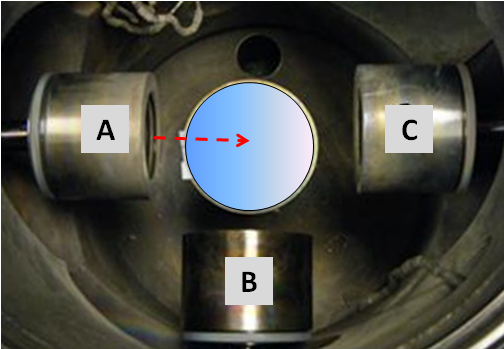
\includegraphics[width=0.7\textwidth]{chapter_2/calibration}
\caption{Guns in the off-axis configuration for deposition rate calibration. Figure depicts a deposition profile along Gun A.}
\label{calibration}
\end{figure}
Three to four equally spaced points on the wafer that are collinear to this line were sufficient to generate an accurate linear thickness profile. An exponentially decaying function was fit to the measured thickness to obtain decay length and thickness at substrate edge. To determine the composition ratio of a binary oxide, we must first convert the thicknesses to molecules per unit area for each elemental oxide using the following equation,
\begin{equation}\label{eq:composition_a}
[A_{x}O_{y}] = t(A_{x}O_{y})*\text{A.M.}(A_{x}O_{y})*\rho (A_{x}O_{y})*N_{a}.
\end{equation}

For elemental oxide $A_{x}O_{y}$,  $t(A_{x}O_{y})$ denotes the thickness from the linear profile, $\text{A.M.}(A_{x}O_{y})$ is the atomic mass of the molecule, $\rho (A_{x}O_{y})$ is the density of the molecule, and $N_{a}$ is Avogadro's number. Once the number of molecules per unit area is determined, the composition ratio of molecule $A_{x}O_{y}$ can be inferred by simply taking a ratio,
\begin{equation}\label{eq:composition_b}
\frac{[A_{x}O_{y}]}{[B_{p}O_{q}]+[A_{x}O_{y}]}
\end{equation}
in which the numerator represents the number of $A_{x}O_{y}$ molecules per unit area, whereas the denominator is the total number of molecules per unit area. The area term automatically cancels out since it is present in both the numerator and denominator. The ratio is only valid when the deposition times are consistent for each calibration.

Although composition profiles are typically highly reproducible (to $\sim$1 at\%), the conditions in the chamber may slightly change day to day affecting film properties between runs, so it is still instructive to perform a direct composition measurement; for this we use WDS. WDS is a sister technique to the EDS (energy-dispersive x-ray spectroscopy) and relies on the interaction of electrons with the material to stimulate emission of x-rays. The emitted x-ray energies are characteristic to the material and therefore in theory, the composition ratios can be discerned.

In comparison to EDS, WDS has a much higher spectral resolution; the resolution of EDS is typically on the order of $\sim$ 100 eV, while WDS can resolve peaks down to several eV at full width half max (FWHM) \cite{Goldstein2003}. Improved resolution in WDS is achieved by preferential diffraction of characteristic x-rays through an analyzing crystal, in which the interaction of the x-rays with the crystal is dictated by Bragg's law, $n\lambda = 2d\sin(\theta)$. The detector, which collects the diffracted x-rays, and the crystal are simultaneously moved such that angle $\theta$ is varied by changing the position of the detector relative to the sample. Varying $\theta$ in turn selects which wavelength is diffracted according to Bragg's law. 

WDS's accuracy is further improved by the use of standards with known composition. The task now is to take the measured intensity from the sample for element $i$, ${I_{i}}$, and compare it to the intensity measured from the standard ${I_{(i)}}$ to determine the composition in the sample. As a first approximation, one can determine the ``k ratio,"
\begin{equation}\label{eq:kratio}
\frac{C_{i}}{C_{(i)}} = \frac{I_{i}}{I_{(i)}} = k_{i}
\end{equation}
which assumes that the ratio between ${I_{i}}$ and ${I_{(i)}}$ determines the mass composition ratio $C_{i}$/$C_{(i)}$, the composition fraction of the element of interest in the sample, and the composition fraction of the element of interest in the standard, respectively. Complicating the analysis are ``matrix effects," e.g. absorption and fluorescence, which have to be taken into account since they lead to errors in the k-ratio. Matrix effects are divided into three effects: atomic number ($Z_{i}$), x-ray absorption ($A_{i}$), and x-ray fluorescence ($F_{i}$). We can obtain the corrected k ratio by multiplying the correction factor for element $i$,
\begin{equation}\label{eq:zaf}
k(\text{corrected})_{i} = k_{i} [ZAF]_{i}.
\end{equation}

\subsection{Measuring film density using x-ray reflectivity}

To calculate the polarizability of the material using the Clausius-Mossotti relation one needs to know the dielectric constant, $\varepsilon_{r}$, and density, $\rho$. While the dielectric constant is easily determined by C-D measurements, the density of an amorphous material is more difficult to ascertain, particularly since we require a systematic evaluation of $\rho$ as a function of composition (position on the wafer). For our study, we rely on x-ray reflectivity (XRR) measurements to probe the density of the material at various points on the wafer. 

X-ray reflectivity works by total external reflection, which occurs when x-rays are shined on a material with an angle of incident ($\theta$) that is less than the critical angle $\theta_{c}$---where the critical angle is typically $\theta_{c}$ $<$ 0.5. Total external reflection only occurs because the refractive index, $n$, of a material is less than one at x-ray wavelengths. Because the condition for total external reflection depends on the electron density of the material, and therefore mass density, measuring the critical angle is an indirect measurement of material density. 

Reflectivity measurements were carried out using the Rigaku Smartlab diffraction system. Sample alignment is crucial to XRR measurements, hence we aligned the sample at each point on the wafer prior to each measurement. Standard 40 keV Cu K-$\alpha$ X-rays were conditioned through a slit assembly to minimize the beam footprint (footprint $\leq$ 10mm$\times$3mm). Note, a large beam footprint is undesirable since we want to minimize the compositional averaging from the sample. In some cases a Ge (220)$\times$2 monochromator was utilized to further minimize the beam footprint. The reflected x-rays were further conditioned by the receiving slit assembly before being collected by the detector. To simplify the analysis, we took the critical angle to be the angle in which the intensity becomes half the total reflected intensity \cite{Parratt1954}. The critical angle is related to the mass density by the following formula 
\begin{equation}
\rho = \frac{\theta_{c}^{2}\pi A}{Zr_{e}\lambda^{2} N_{A}} 
\label{eq:rho}
\end{equation}
where $A$ is the atomic mass unit, $r_{e}$ the classical electron radius, $\lambda$ the x-ray wavelength, $N_{A}$ is Avogadro's number, and $Z$ the atomic number \cite{Bahr1993}. Intrinsic to this equation is the assumption that $\theta_{c} = \sqrt{2\delta}$, which requires that the atomic form factor $f^{0}_{1}$ $\approx$ $Z$ and that  $f^{0}_{2} << f^{0}_{1}$. These are fairly reasonable assumptions to make at these x-ray energies \cite{Chantler1995}.

\section{Structural characterization of non-crystalline materials}

The Merriam-Webster Webster dictionary defines the word amorphous as "having no definite form," suggesting that amorphous materials lack any kind of ordering. However, this is far from the truth. In fact, amorphous materials consist of recurring structural elements that exhibit ordering in short range (typically several nearest neighbor distances). The complexity of the matter is evidenced, for example, by the on-going debate over the structural topology of amorphous Si \cite{Treacy2012}. The fact is, it merely appears that amorphous materials lack ordering because conventional methods that probe structure (e.g. x-ray diffraction using Cu-K$\alpha$ radiation) are typically not able to uncover short or even medium range order. Therefore, researchers must rely on more specialized methods \cite{Cockayne2007} to unravel the ``hidden" structure of amorphous materials. 

\subsection{Real space diffraction}

We rely heavily on several preexisting techniques that have experienced historic development, one of which is real space diffraction analysis. The goal of the technique is to determine a pair distribution function (PDF), $g(r)$, that represents the probability of finding an atom at distance $r$ from an origin atom. Several references on this topic are available \cite{Billinge2003,Warren1990,Waseda1980, Farrow2009}. To obtain $g(r)$ we must compute $\varphi(Q)$, the reduced intensity function from measured X-ray intensities, $I(Q)$, and then apply a sine Fourier transform. The canonical expression of the PDF is,
\begin{equation}\label{eq:PDF}
g(r) =\rho_{a} + \frac{1}{2\pi^{2}r} \int_{0}^{\infty} \varphi(Q)\sin{Qr}\;dQ.
\end{equation} 
Binary alloys require further mathematical treatment (to extract partial distribution functions for proper structural analysis), and ternary even more so. Recent improvements in computational power allow modeling of complex amorphous systems with great accuracy \cite{Petkov1998, Bassiri2011}, and can be used in conjunction with experimental data to determine partial distribution functions. In the following section we derive the PDF for the simple case of a single element system, similar to the derivation found in \cite{Warren1990}.  

In the kinematical limit the scattering intensity is written as the sum of amplitudes from different atoms multiplied by its complex conjugate. Defining a difference vector $\textbf{r}_{ji} = \textbf{r}_{j} - \textbf{r}_{i}$:
\begin{equation}\label{eq:ScatI}
I(Q) = \sum_{j}\sum_{i} f_{j}f_{i} e^{(2\pi i/\lambda) (\textbf{s}-\textbf{s}_{0}) \cdot \textbf{r}_{ji}}.
\end{equation}
We can separate the sums for terms where $i=j$
\begin{equation}\label{eq:Ic1}
I(Q) = \sum_{j}f^{2}+ \sum_{j}f^{2}\sum_{i\neq j} e^{(2\pi i/\lambda) (\textbf{s}-\textbf{s}_{0}) \cdot \textbf{r}_{ij}}.
\end{equation}
Introducing a density function $g_{j}(\textbf{r}_{ij})$ we can write the the sum for the $i\neq j$ term as an integral over the volume element $dV$
\begin{equation}\label{eq:Ic2}
I(Q) = \sum_{j}f^{2}+ \sum_{j}f^{2}\int g_{m}(\textbf{r}_{ij})e^{(2\pi i/\lambda) (\textbf{s}-\textbf{s}_{0}) \cdot \textbf{r}_{ij}}dV.
\end{equation}
Adding and subtracting the average atom density in the sample $\rho_{a}$, we obtain two integrals over the sample volume:
\begin{equation}\label{eq:Ic3}
I(Q) = \sum_{j}f^{2}+ \sum_{j}f^{2}\int [g_{m}(\textbf{r}_{ij})-\rho_{a}]e^{(2\pi i/\lambda) (\textbf{s}-\textbf{s}_{0}) \cdot \textbf{r}_{ij}}dV + \sum_{j}f^{2}\int \rho_{a}e^{(2\pi i/\lambda) (\textbf{s}-\textbf{s}_{0}) \cdot \textbf{r}_{ij}}dV.
\end{equation}
To solve the integral we take an orientational average over the volume of the sample, assuming an isotropic distribution of atoms. The average density function is $g(\textbf{r}) = \langle g_{j}(\textbf{r}_{ij})\rangle$, in which $\textbf{r} = \textbf{r}_{ij}$ for fixed atom displacements. We consider amorphous materials of the type such that for large $\textbf{r}$ values, $g(\textbf{r}) - \rho_{a}$ goes to zero. We can thus simplify the sum of the self-scattering terms by replacing the sum with $N$. Also, the third term only contributes to I(Q) at small scattering vectors, so it can be dropped from the equation if small angles are not included in the data. Substituting the scattering vector $Q = 4\pi \sin{\theta/\lambda}$, and from the fact that 
$(\textbf{s} - \textbf{s}_{o})\cdot(\textbf{r}_{nm}) = 2\sin{\theta}\;r\cos{\phi}$, we can solve the integral in equation \ref{eq:Ic3}
\begin{equation}\label{eq:Ic4}
I(Q) = Nf^{2}+ Nf^{2}\int^{\infty}_{0}\int^{\pi}_{0}[g(r)-\rho_{a}] e^{ikr\cos{\phi}}2\pi r^{2} \sin{\phi}\;d\phi\;dr
\end{equation}
\begin{equation}\label{eq:Ic5}
I(Q) = Nf^{2}+ Nf^{2}\int^{\infty}_{0} 4\pi r^{2}[g(r) - \rho_{a}] \frac{\sin{kr}}{kr}\;dr.
\end{equation} 
To get the PDF we introduce the reduced intensity function $\varphi(Q)$
\begin{equation}\label{eq:RIF}
\varphi(Q) = \left[\frac{I(Q) - Nf^{2}(Q)}{Nf^{2}(Q)}\right]Q
\end{equation}
which gives us, 
\begin{equation}\label{eq:phi}
\varphi(Q) = 4\pi\int^{\infty}_{0}  r[g(r) - \rho_{a}] \sin{kr}dr.
\end{equation}
Currently phi is a function of Q-space. The PDF is a real space function and therefore, we need to apply a Fourier transform to $\varphi(Q)$. Defining $f(r) =  r[g(r) - \rho_{a}]$, we obtain the following Fourier pair:
\begin{equation}\label{eq:pair}
\begin{split}
 & \varphi(Q) = 4\pi\int^{\infty}_{0} f(r) \sin{kr}\;dr\\
 & f(Q) = \frac{1}{2\pi^{2}}\int^{\infty}_{0} \varphi(Q) \sin{kr}\;dr.
\end{split}
\end{equation}
From this we see that with a little rearranging, one can easily obtain the result presented in equation \ref{eq:PDF}.
Experimentally, the challenge lies in accurately measuring the scattered intensity $I(Q)$ and applying the proper correction algorithms such that an accurate PDF can be obtained. All diffraction spectra in this study were obtained at the Cornell High Energy Synchrotron Source (CHESS) A2 line at 40keV, corresponding to an x-ray wavelength of 0.030657 nm.

\subsection{Silicon nitride membranes for x-ray diffraction}

*Silicon nitride membranes were designed and fabricated by Lauren Taylor*

\noindent The signal from the silicon diffuse scattering adds an extra step in the data reduction process when characterizing thin films deposited on single crystal silicon in transmission \cite{Gregoire2009a}. For amorphous materials, this extra signal from silicon diffuse scattering is especially problematic since the captured signal from the amorphous materials are not as intense in comparison to crystalline materials. To circumvent this problem altogether, we mainly performed scattering experiments on films that were deposited on amorphous silicon nitride membranes. Because the nitride membranes are thin (a few microns thick) and amorphous, the subtraction process can be performed with greater ease.

Silicon nitride membrane arrays were fabricated using standard clean room processes in Cornell's Nanofabrication Facility (CNF). The membranes were arranged in a two-dimensional array as shown in Figure \ref{windows}. 
Window size was modified depending on the number of membranes in the array. The windows for the 12$\times$12 array were 2 mm on each side, whereas the windows for the 8$\times$8 and 9$\times$9 arrays were 3 mm.

\begin{figure}
\centering
\noindent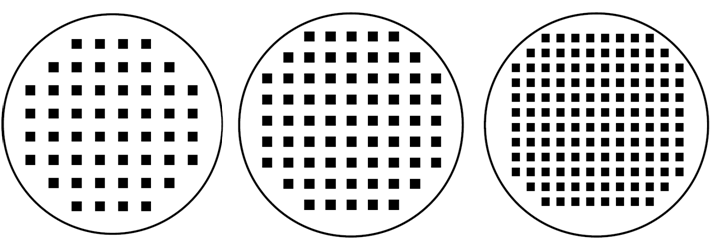
\includegraphics[width=\textwidth]{chapter_2/windows}
\caption{Cartoon showing the different silicon nitride membrane arrays used for the diffraction studies. From left to right: 8$\times$8, 9$\times$9, and 12$\times$12 arrays.}
\label{windows}
\end{figure}

Prior to silicon nitride deposition, 3 inch double-side polished wafers were cleaned in an acid bath followed by a base bath and rinsed in deionized water after each. The wafers were then transferred to an MRL Industries low pressure chemical vapor deposition (LPCVD) furnace where low stress silicon nitride was deposited. The nitride deposition rate was approximately 30 \AA\;per minute determined from prior calibration runs. The substrates were kept in the furnace for 7 hours at 775 \textdegree C, which yielded nitride films that were approximately 1.5-1.6 microns thick determined by reflectometry (FilMetrics Film Measurement System). Window array patterns were developed on the wafer using standard photolithographic methods. This involves transferring a photoresist pattern of the array onto the nitride coated substrate and etching away the nitride in the exposed windows. Finally, the wafer was back-etched using a potassium hydroxide solution forming the silicon nitride windows.

\subsection{From measured intensity to PDF}

Data acquisition is only half the battle, the other being data reduction and analysis. To refine the raw data into something we can analyze, we first normalized to the total x-ray flux (IC3 counts) and subtracted the silicon nitride background from the raw 2D spectra. The spectra was then collapsed into a 1D diffraction pattern by integrating azimuthally in fit2D \cite{Hammersley1996}.

At this point it is common to apply further corrections to the diffraction pattern. This includes polarization, absorption, multiple scattering effects, etc., and have been widely implemented in several PDF analysis programs \cite{Qiu2004}. However, it is fairly time consuming to master these programs and careful consideration of the various errors in diffraction analysis is required, calling on a high level of expertise. In this study we make use of a less arduous approach by analyzing the data \emph{ad hoc}. 

The \emph{ad hoc} approach is possible because of certain general properties of the structure function. Corrections to measured intensity, $I_{m}(Q)$, are expected to be  either additive or multiplicative,
\begin{equation}
I_{c}(Q) = a(Q)I_{m}(Q) + b(Q)
\label{eq:Im}
\end{equation}
where $a(Q)$ and $b(Q)$ are the Q dependent multiplicative and additive factors to the measured intensity, which if varied appropriately, gives us the correct form of the coherent scattered intensity, $I_{c}(Q)$. The correction factors can also be related to the total scattering structure function $F(Q)$ (as denoted by some researchers), essentially equivalent to $\varphi(Q)$ found in Equation \ref{eq:RIF}
\begin{equation}
F(Q) = \alpha(Q)I_{m}(Q) + \beta(Q).
\label{eq:F{Q}}
\end{equation}
The critical insight is that although $\alpha(Q)$ and $\beta(Q)$ are not known \emph{a priori}, the general form and behavior of the correction factors are known. Hence, the correct forms of $\alpha(Q)$ and $\beta(Q)$ can be determined variationally using PDFgetX3 \cite{Juhas2013a}.

We feed the background subtracted diffraction patterns into PDFgetX3 using the Python based command-line interpreter \cite{Juhas2013a}. The program then variationally adjusts the correction factors and applies a sin Fourier transform to $F(Q)$ to solve for the PDF:
\begin{equation}\label{eq:pdf}
g(r) = \frac{2}{\pi} \int_{Q_{min}}^{Q_{max}} F(Q) \sin{Qr} dQ.
\end{equation}
Note, that because we cannot collect data to infinite wavelengths, $Q_{max}$ is always a finite value. This is equivalent to convolving a step function beyond $Q_{max}$, which becomes convolved with the data, resulting in ``truncation" errors. In order to reduce this error, researchers typically collect data to sufficiently large Q values to incorporate a large number of Fourier components to perform the transform \cite{Dykhne2011}.

Direct information such as bond distance and coordination number are immediately available from the refined PDF. As mentioned earlier a more involved, but illuminating approach is simulating the amorphous structure \cite{Zhang2007, Bassiri2011}. This enables us to not only confirm what we learn from the direct analysis, but also ascertain additional information such as the partial distribution functions for multicomponent systems and electrical properties such as the dielectric constant.

\subsection{X-ray absorption fine structure}

The PDF method provides us with valuable local structural information. Nonetheless, the technique is not element specific. X-ray absorption fine structure (EXAFS, or XAFS)---a method which falls under X-ray absorption spectroscopy (XAS)---is an \emph{element specific} local probe of the material, which can be used to extract information much like the PDF method and further, gather chemical information about the material such as the valence state of an element. 

EXAFS capitalizes on the wave-particle behavior of electrons. Within the x-ray energies we are interested in (1 $\leq$ E $\leq$ 100 keV), x-rays are absorbed by the photoelectric effect. Absorption of the x-ray excites an electron out of the atom leaving a core-hole. The element specificity is achieved by tuning the energy of the x-ray such that we only look at the absorption event for a specific element. Several events can also follow the absorption process such as the annihilation of the core-hole via fluorescence, or the emission of an Auger electron through an Auger process. The absorption of the x-ray results in the attenuation of the original x-ray intensity, $I_{o}$ to $I$, which is measured by the detector. The relation between $I_{o}$ and $I$ can be expressed by the Beer-Lambert law 
\begin{equation}
I = I_{o}e^{-\mu(E) t}
\label{eq:BL}
\end{equation}
in which the absorption coefficient $\mu(E)$ is also an energy dependent quantity. The presence of neighboring atoms scatters the emitted photo-electron and in this process interferes with other scattered photo-electrons. This interference effect produces fringing in the absorption coefficient known as the ``fine structure," which provides information about the local environment in the material. We can write the fine structure in terms of the absorption coefficients,
\begin{equation} 
\chi(E) = \frac{\mu(E) - \mu_{o}(E)}{\Delta\mu_{o}(E_{o})}
\label{eq:EXAFS_chi}
\end{equation}
where $\mu_{o}(E)$ is the background absorption and $\Delta\mu_{o}(E_{o})$ is the edge step which normalizes the equation to one absorption event. We can extract useful information from the data by modeling the fine structure. Taking into account inelastic and multiple scattering and thermal vibrations the EXAFS equation is
\begin{equation} 
\chi(k) = \sum_{i}\frac{N_{i}S_{o}^{2}f_{i}e^{-2R_{i}/\lambda(k)}e^{-2k^{2}\sigma_{i}^{2}}}{kR^{2}_{i}} \sin{2kR_{i} + \delta_{i}(k)}.
\label{eq:exafs2}
\end{equation}
Here, we have expressed the EXAFS as a function of the photo-electron wave number $k = \sqrt{\frac{2m(E-E_{o})}{\hbar}}$. By fitting to the EXAFS equation, we can extract information such as bond distance and coordination number centered around a specific element. 

All EXAFS experiments were carried out in CHESS's F3 line. We tuned the energy of the x-rays to the desired absorption edge (Ta L-3 absorption edge for tantalum based materials which sits at $\sim$9883 eV). Ta metal foil was also used to calibrate the absorption edge. Data reduction and analysis was performed using the ATHENA and ARTEMIS software packages \cite{Ravel2005}.


% chapter 3
\chapter{Dielectric Properties of Amorphous Zr-Al-O and Zr-Si-O Thin Films}

{\let\thefootnote\relax\footnote{{
This work was published to \emph{Journal of Advanced Dielectrics}. Reprinted with permission from \cite{Naoi2015}.
}}}

\section{Abstract}
We have systematically studied the composition dependence of the dielectric properties of $\textnormal{Zr}_{1-x}\textnormal{Al}_{x}\textnormal{O}_{2-x/2}$ and $\textnormal{Zr}_{1-x}\textnormal{Si}_{x}\textnormal{O}_{2}$.
An essentially linear variation of the static dielectric constant, $\varepsilon_s$, was observed as a function of composition, $x$, for compositions rich in the p-block element, i.e., $x>0.4$, for both chemical systems. However an abrupt change in $\varepsilon_s$ is found near $x \approx 0.35$, associated with the onset of crystallinity in as-deposited films. Breakdown fields do not show a comparable composition dependence. Measurements of the index of refraction at optical frequencies, combined with a simple Clausius-Mossotti interpretation, indicates that low-frequency (ionic) contributions to the polarizability exhibit systematic deviation with respect to values linearly interpolated from the endmembers. These trends are not consistently affected by the presence of crystalline order, but are related to changes associated with heterogeneous local oxygen coordination and bonding.

\section{Introduction}
Amorphous  dielectrics comprising mixed transition-metal/p-block (e.g., Hf, Zr or Ta combined with Al, Si or Ge) oxides are technologically important and are generally viewed as following simple trends as a function of composition. Some examples (e.g., Zr-Si-O) have been found to exhibit unexpected behavior, such as an enhanced dielectric constant \cite{Wilk2000,Wilk2001,Lucovsky2000,Naoi2012}.
Amorphous \ce{HfO2}-based dielectrics, modified with the addition of \ce{SiO2} and/or \ce{Al2O3}, are now widely used in commercial integrated circuits as alternatives to the native \ce{SiO2} dielectric that controls charge transport in Si-channel field-effect transistors, because \ce{HfO2}, like other oxides of the Group 3, 4, and 5 elements, has a significantly higher dielectric constant (static value of the relative dielectric constant, $\varepsilon_s = \varepsilon (\omega \rightarrow 0)/\varepsilon_0 \approx 23$) than \ce{SiO2} for which $\varepsilon_s \approx 3.9$. 
Compared to \ce{SiO2} they can therefore achieve a comparable charge density at a specified gate voltage using a layer thick enough to avoid excessive leakage by direct tunneling \cite{Kingon2000}. Ab-initio studies of amorphous $\textnormal{Zr}_{1-x}\textnormal{Si}_{x}\textnormal{O}_{2}$ and $\textnormal{Hf}_{1-x}\textnormal{Si}_{x}\textnormal{O}_{2}$ and related materials have highlighted the importance of local structure on dielectric properties, and the consequent impact on the composition dependence \cite{Pignedoli2007,Nakamura2005,Rignanese2002,Ouyang2005}.

In order to understand the behavior of this interesting class of materials, we have focused on the Zr-Al-O and Zr-Si-O systems. Films deposited at room temperature exhibit a clear transition from nanocrystalline (Zr-rich compositions) to amorphous (Si- or Al-rich compositions). Polycrystalline and amorphous thin films of these materials exhibit comparable values for $\varepsilon_{s}$; in both case the value represents an approximate directional average of the anisotropic value associated with single crystals. The question of crystallinity can be important; for example, as gate dielectrics, amorphous oxides are advantageous over polycrystalline materials since they avoid inhomogeneity in local charge density due to anisotropy that would degrade mobility in the conducting channel of an FET. Polycrystalline dielectrics are expected to exhibit a lower breakdown field than that of amorphous dielectrics due to the presence of grain boundaries \cite{Lanza2012}. %=reference suggesting grain boundaries lead to low breakdown
We are using these two systems to determine the effect of the presence or absence of crystallinity on the dielectric constant and the breakdown field, and to determine the systematic effect of the Zr/Si or Zr/Al ratio on these properties. This information provides insight regarding the mechanism for the observed enhancement of the dielectric response. 

We used a composition-spread technique for thin film growth to enable composition-dependent trends to be identified with low composition-to-composition process variation and very fine composition resolution. The dielectric constant of amorphous films was found to vary roughly linearly with composition, while the static dielectric constant of crystalline (transition-metal-rich) films was found to be significantly higher. Leakage currents and breakdown fields were less strongly composition dependent and suggest that grain boundaries in nanocrystalline samples do not serve as weak links.

\section{Experimental Methods}
%Sputtering
Compositionally-graded films were prepared using 90$\degree$
off-axis reactive cosputtering using two 2-inch planar magnetron sputter guns arranged in a facing-targets configuration,
as described previously \cite{vanDover1999}.
The 75 mm diameter Si substrates were positioned
between the two guns so that species sputtered from each
target condense on the substrate simultaneously. The
deposition rate decreases rapidly as a function of distance from
the target, so a natural composition gradient is obtained in this geometry \cite{vanDover1999}.
The sputter guns were operated at rf power levels chosen to achieve approximately 1:1 cation ratio at the center of the substrate.
The films were about 100 nm thick with cations randomly mixed on an atomic scale. Films used for evaluation of crystallinity were deposited on bare Si wafers while those used for evaluation of electrical and optical properties were deposited on wafers pre-coated with sputtered TiN).
Prior to film deposition the vacuum chamber was evacuated to a pressure of 10$^{-6}$ Torr or lower.  Gas flow rates during deposition were 15 std. $\textnormal{cm}^3 / \textnormal{minute}$ (sccm) Ar and 10 sccm \ce{O2}, with the turbopump throttled to maintain a pressure of 30 mTorr in the chamber.  
The substrate was also intentionally biased with 10 W rf power, yielding a dc potential of -75 V that ensures formation of a dense film (avoiding formation of columnar voids during deposition \cite{Barron2009}.)
The substrate temperature during deposition was maintained below 60 \textdegree C by attaching the substrate to a heatsink. Under these conditions the deposition rate was roughly 0.1 nm/s,though the rate varies somewhat with position on the sample.  The final thickness of the films was on the order of 100 nm.  

%composition
The composition of the films intentionally varies along the length of the sample.  Quantitative composition variation was determined using calibration samples on which a single element was reactively sputtered under the same conditions used for the cosputtered spreads.  The thickness of the deposited film, measured as a function of position using a profilometer, was used to calculate the deposition rate.  The cation composition of the cosputtered sample is then inferred simply by calculating the ratio of arrival rates of the two cation species.  The oxygen stoichiometry in these systems was calculated using charge balance assuming cations are in their highest oxidation state, an assumption that is validated by the observation of low leakage currents in the dielectric. An example of the position dependence of composition is shown in Fig. \ref{ZrAlO_compositions_RBS}.  At selected positions the codeposited samples were examined using Rutherford Backscattering Spectroscopy (RBS).  The RBS analysis, which has an absolute accuracy estimated to be better than 5\%, yielded compositions that were consistent with the results of the rate calibrations, confirming the validity of all of the assumptions inherent in the latter technique.  A typical RBS spectrum is shown in the inset to Fig. \ref{ZrAlO_compositions_RBS}.

The thickness of the films is not strictly constant across the length of the sample, since the sum of the deposition rates from the two targets is not constant.  The thickness was therefore determined as a function of position by preparing a codeposited sample with a liftoff mask.  The mask was then removed and the thickness of the deposited film was determined at fifteen positions using a profilometer.  These measurements of the dependence of thickness with position were interpolated using a quadratic fit.

\begin{figure}
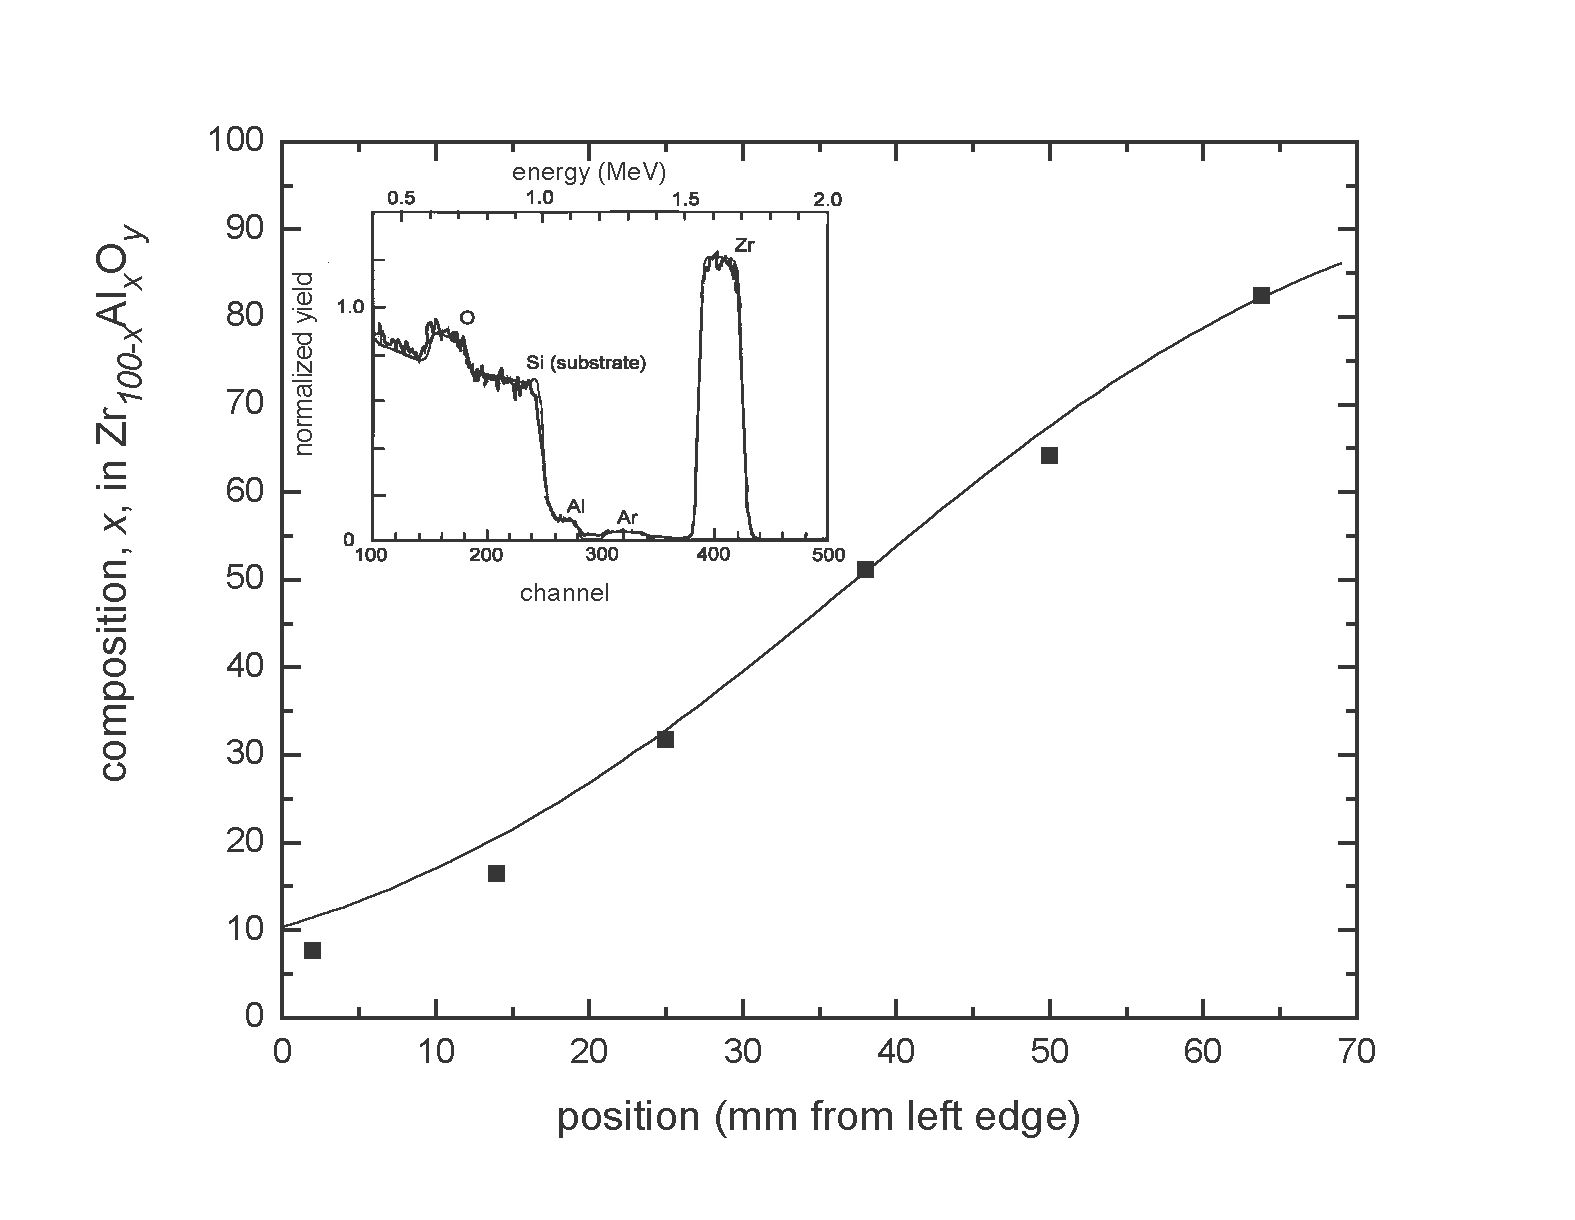
\includegraphics[width=\linewidth]{chapter_3/ZrAlO_compositions_RBS}
\caption{Composition as a function of position along the 7-cm sample axis.  Solid line: compositions calculated using rate calibrations for each species (\ce{ZrO2}, \ce{Al2O3}).  Squares: Compositions inferred using Rutherford Backscattering Spectroscopy.  Inset: a typical RBS spectrum used to determine the composition. A small level of Ar incorporation is typical in sputtered films, and can be seen in the RBS spectrum, though it has a negligible effect on electrical or structural properties.}
\label{ZrAlO_compositions_RBS}
\end{figure}
%XRD
X-ray diffraction patterns were taken with a Brucker-AXS system equipped with a Cu $K_\alpha$ generator and crossed-wire area (two-dimensional) detector.
The resulting data were integrated over the range -47$\degree$ $ < \chi < $ -133$\degree$ to yield a single graph of integrated intensity versus $2\theta$. 
The crystallites exhibited no preferred orientation. 
Fig. \ref{ZrAlO_ZrSiO_XRD} illustrates the reflections associated with monoclinic \ce{ZrO2}, observed for Zr-rich compositions that exhibit nanoscale crystalline order.
The width of the peaks, corrected for instrument resolution, is a measure of the crystallite size (structural coherence length, $L$) as inferred using the Debye-Scherrer formula, $L = 0.6 \lambda / B cos \theta$, where $B$ is the full width at half maximum.  
The pattern corresponding to $\textnormal{Zr}_{0.75}\textnormal{Si}_{0.25}\textnormal{O}_{2}$ is marked with the $(hkl)$ Miller indices of the monoclinic phase; the distinct peak expected for cubic or tetragonal \ce{ZrO2} at approximately 30$\degree$ is clearly not present in the pattern. 
The pattern corresponding to $\textnormal{Zr}_{0.89}\textnormal{Al}_{0.11}\textnormal{O}_{1.94}$ is less well defined, but is consistent with monoclinic \ce{ZrO2}.
It is surprising that the monoclinic phase should be present in nanocrystalline $\textnormal{Zr}_{0.89}\textnormal{Al}_{0.11}\textnormal{O}_{1.94}$, both because incorporation of a trivalent ion in \ce{ZrO2} introduces O vacancies that typically stabilize the cubic fluorite phase, as in yttrium-stabilized zirconia, and because grain refinement in unsubstituted \ce{ZrO2} also stabilizes the cubic phase \cite{Gupta}.
When an identical $\textnormal{Zr}_{1-x}\textnormal{Al}_{x}\textnormal{O}_{2-x/2}$ composition spread was annealed at 1000 \textdegree C for 20 seconds in \ce{N2}, Zr-rich compositions ($x<0.18$) exhibited a mixture of monoclinic and tetragonal phases while for $0.18 < x < 0.40$ the structure was entirely cubic, a result that is not inconsistent with expected equilibrium behavior. For $x>0.4$ a mixture of cubic and amorphous material was present.
Annealing  $\textnormal{Zr}_{1-x}\textnormal{Si}_{x}\textnormal{O}_{2}$ at 1000\textdegree C yielded surprisingly similar results, considering that tetravalent Si will not introduce O vacancies to maintain charge balance. 
Zr-rich compositions ($x<0.35$) exhibited a mixture of monoclinic and tetragonal phases while for $0.35 < x < 0.80$ the structure is entirely cubic. 
Apparently introduction of Si, which favors tetrahedral coordination with O (rather than the octahedral coordination of \ce{ZrO2}), disrupts the interactions that stabilize the monoclinic structure. Interestingly, no evidence for formation of zircon, \ce{ZrSiO4}, is observed in the annealed films \cite{VanDover2003}.     
%
\begin{figure}
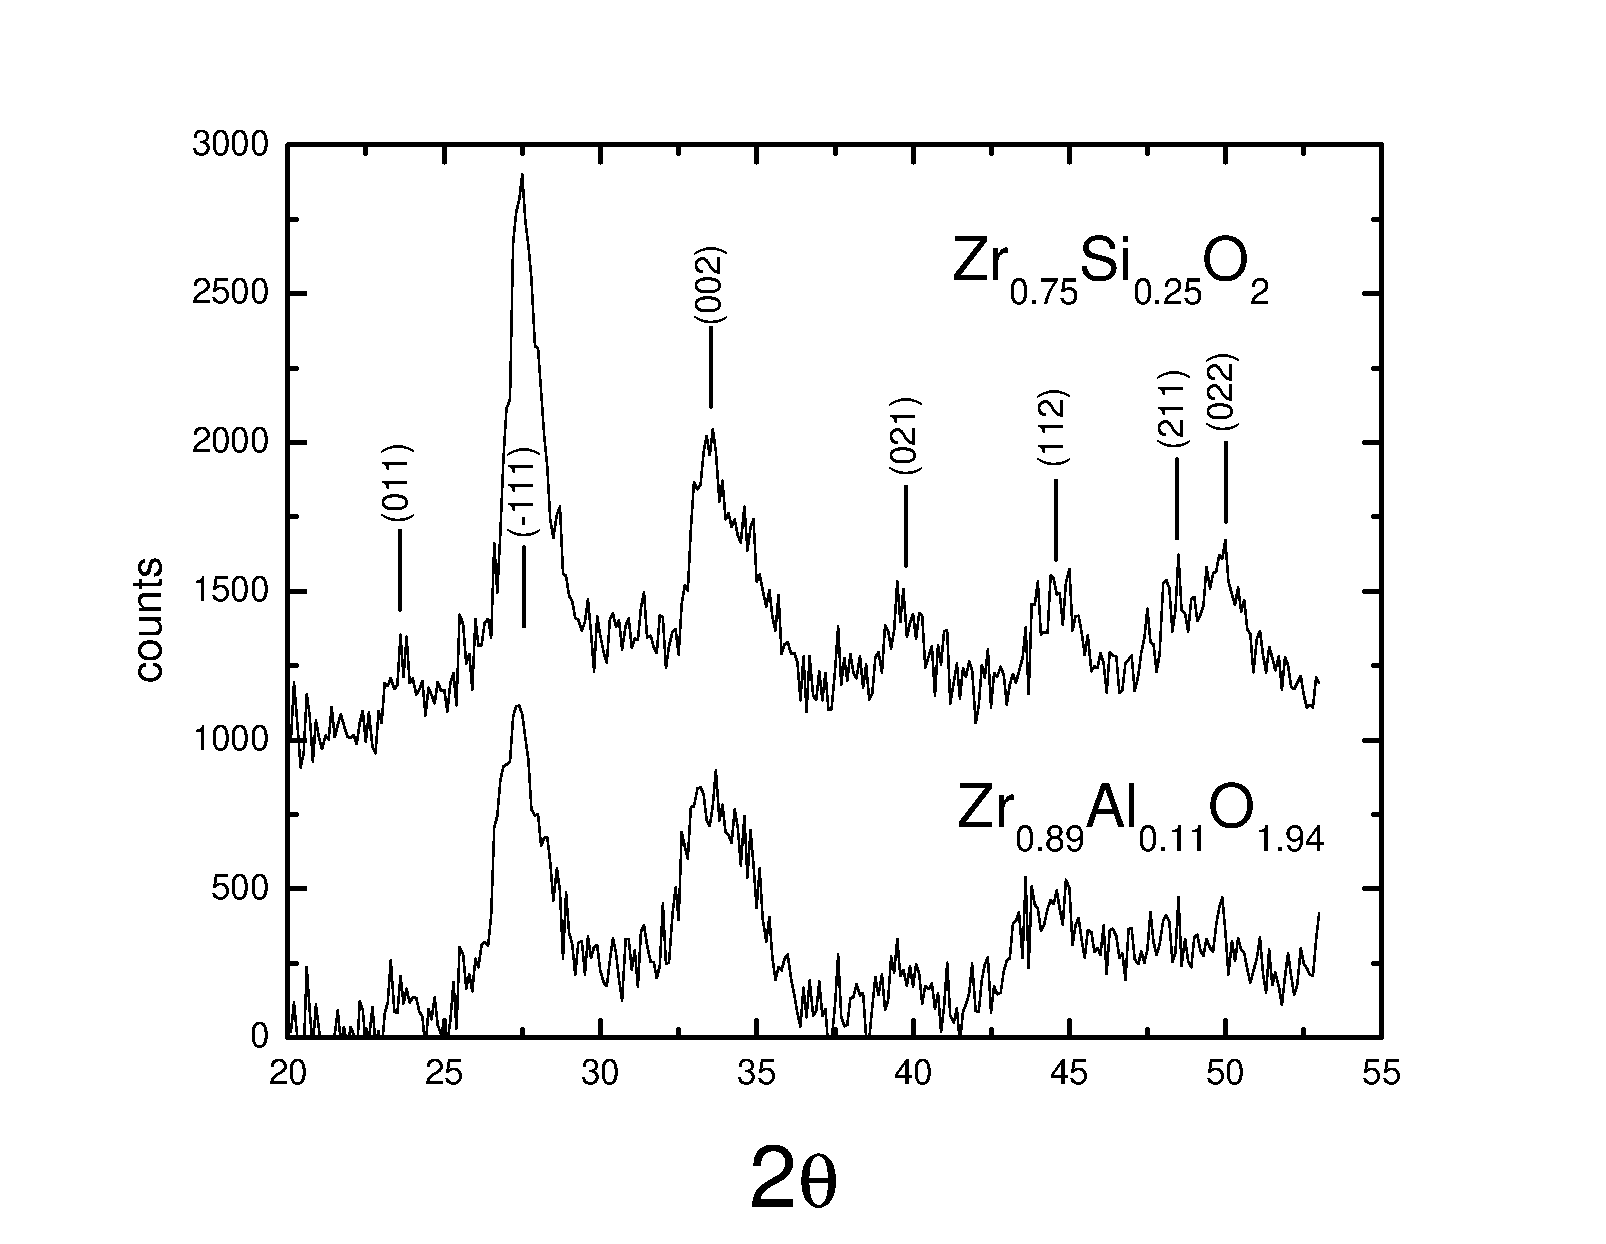
\includegraphics[width=\linewidth]{chapter_3/ZrAlO_ZrSiO_XRD}
\caption{X-ray diffraction patterns for typical nanocrystalline Zr-rich samples. Top curve:  $Zr_{0.75}Si_{0.25}O_2$ film as deposited, offset vertically for clarity, with positions for the strongest monoclinic reflections indicated. Bottom curve: $Zr_{0.89}Al_{0.11}O_{1.94}$, illustrating x-ray peaks that are broader due to the lower degree of crystallinity compared to the Zr-Si-O sample.}
\label{ZrAlO_ZrSiO_XRD}
\end{figure}	


%Ellipsometry
The index of refraction and thickness of the films were determined using a Sentech SE801 spectroscopic ellipsometer over a wavelength range of 450-800 nm. The optical constants of the substrate layer were determined prior to film deposition and were fixed during the fitting process. A film/substrate bilayer model was used to fit $\psi$ and $\delta$, and the optical constants of the film were modeled using the Cauchy relation $n(\lambda) =  n_0 + n_1 / \lambda^{2} + n_2 / \lambda^{4}$ using a least-squares routine. The reported refractive index $n$ was taken to be $n_{0}$, i.e., the infinite wavelength limit far from absorption edge.
%

%Electical properties
The static dielectric constant, $\varepsilon_s$ was evaluated using parallel-plate capacitors fabricated on oxide films grown on a non-reactive TiN base electrode.  Pt counterelectrodes 20 nm thick and 200 $\mu$m in diameter were deposited on the films using electron-beam evaporation through a shadow mask.  
The capacitance of these structures was measured at 10 kHz using an automated probing station and an HP4192A capacitance meter.  Some capacitors were measured from 100 Hz to 1 MHz, and were found to exhibit little dispersion over this range. The dissipation factor for all compositions was found to be low ($\tan\delta < 0.05$), indicating high quality films with no anomalous polarization modes \cite{Barron2009}.
Typically 10 to 40  capacitors were measured at each composition in the linear composition spread; the median value was chosen as representative.
Current-voltage characteristics were also measured on the Pt/dielectric/TiN capacitor structures. 
A Keithley 617 source/electrometer was used to apply a stepped voltage across the capacitor and to measure the resulting leakage current. 
Fields from 0 to 10  MV/cm were applied (Pt counterelectrode biased positively), and current densities in the range $10^{-7}$ -- $10^{-3} A/cm^{2}$ were measured.  The breakdown field, $E_{br}$, was defined as the field at which the current density increased by a factor of 100 or more in a single ~0.1 MV/cm step. 
In cases where the I-V curve was continuous even up to $10^{-3} A/cm^2$ (soft breakdown), the breakdown criterion was chosen to simply be the field at which the current density passed $10^{-4} A/cm^2$. 
Again, 10 to 40 capacitors were measured at each composition; because random defects are unavoidable in films fabricated and processed in a non-cleanroom facility we chose the maximum measured $E_{br}$ as the best representative of the intrinsic behavior of the dielectric.

\section{Results and Discussion}
\subsection{Dielectric constant and refractive index}
The composition dependence of the dielectric constant of $\textnormal{Zr}_{\textnormal{x}}\textnormal{Al}_{\textnormal{1-x}}\textnormal{O}_{\textnormal{1.5+x/2}}$ is presented in Fig.
\ref{ZrAlO_epsilon_cohere}. 
Marks at $x=0$ and $x=1.0$ represent expected values for the endmembers. The dielectric constant of \ce{Al2O3} ($\varepsilon_s \approx 9$) is not controversial \cite{Shannon1993a}.
The dielectric constant of monoclinic \ce{ZrO2} appears to be $\varepsilon_s \approx 32$ based on extrapolation of data measured on polycrystalline ceramic (Zr,Y)O$_{\textnormal{x}}$ as reported by Henn, et al. \cite{Henn1995}.
We note that another reference suggests $\varepsilon_s \approx 17$ based on interpretation of infrared spectroscopy \cite{Feinberg}
and supported by first-principles calculations \cite{Zhao2002}.
We note also that these calculations predict that metastable phases of \ce{ZrO2} would have distinctly different values for $\varepsilon_s$, namely $\varepsilon_s \approx 37$ and $\varepsilon_s \approx 47$ for the cubic and monoclinic phases \cite{Zhao2002}.
Other \emph{ab initio} calculations \cite{Vanderbilt2005} predict a value $\varepsilon \approx 21$ for amorphous \ce{ZrO2}
which we have marked on the left-hand axis. 
 
The dielectric constant for amorphous (Al-rich) compositions follows a nearly linear interpolation between the values for the amorphous endmembers. A clear jump in $\varepsilon_s$ is seen at approximately $x=0.35$. 
The transition is associated with the change in crystallinity, as suggested by the top panel of Fig. \ref{ZrAlO_epsilon_cohere}, which reports the XRD coherence length (grain size) as a function of composition: the as-deposited films are completely amorphous for $x \gtrsim 0.35$.
Extrapolating data for $x<0.30$ to the left-hand axis yields a value in good agreement with that inferred for monoclinic \ce{ZrO2}.

\begin{figure}
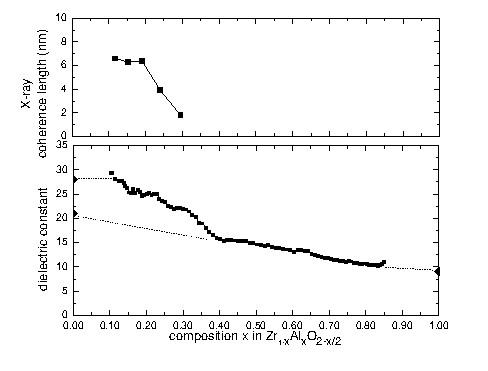
\includegraphics[width=\linewidth]{chapter_3/ZrAlO_epsilon_coherence_1}
\caption{Bottom: Composition dependence of the dielectric constant of thin film $\textnormal{Zr}_{1-x}\textnormal{Al}_{x}\textnormal{O}_{1.5+x/2}$ deposited at room temperature. 
Dotted lines represent extrapolations to values for the endmembers (crystalline and amorphous \ce{ZrO2} and amorphous \ce{Al2O3}) indicated with triangles.Top: composition dependence of the structural coherence length (i.e., essentially grain size) as inferred from X-ray diffraction data using the Debye-Scherrer formula. }
\label{ZrAlO_epsilon_cohere}
\end{figure}

The $\textnormal{Zr}_{1-x}\textnormal{Si}_{x}\textnormal{O}_{2}$ system exhibits a similar behavior as illustrated in Fig. \ref{ZrSiO_eps_cohere}. 
Although the dielectric constant exhibits a nearly linear trend with composition for amorphous compositions ($0.35 < x < 0.90$) and the trend extrapolates to the measured value for \ce{SiO2} ($\varepsilon_s = 3.9$), for $x = 0$ it extrapolates to $\varepsilon_s = 24$ rather than the measured value for amorphous \ce{ZrO2}. 
As in the Zr-Al-O system the abrupt transition in the trend of $\varepsilon_s$ with composition at $x \approx 0.35$ is associated with the change from crystalline to amorphous structure (Fig. \ref{ZrSiO_eps_cohere}, top panel).  
At $x = 0$ the extrapolation of the trend exhibited by crystalline compositions of both Zr-Si-O and Zr-Al-O yields the same value, $\varepsilon_s = 30$, for both, suggesting a common origin. 
However, we note that the crystal structure observed in these films is not the cubic structure bulk \ce{ZrO2} described by Scott, which also extrapolates to $\varepsilon_s = 30$ for undoped \ce{ZrO2}, perhaps coincidentally.   

\begin{figure}
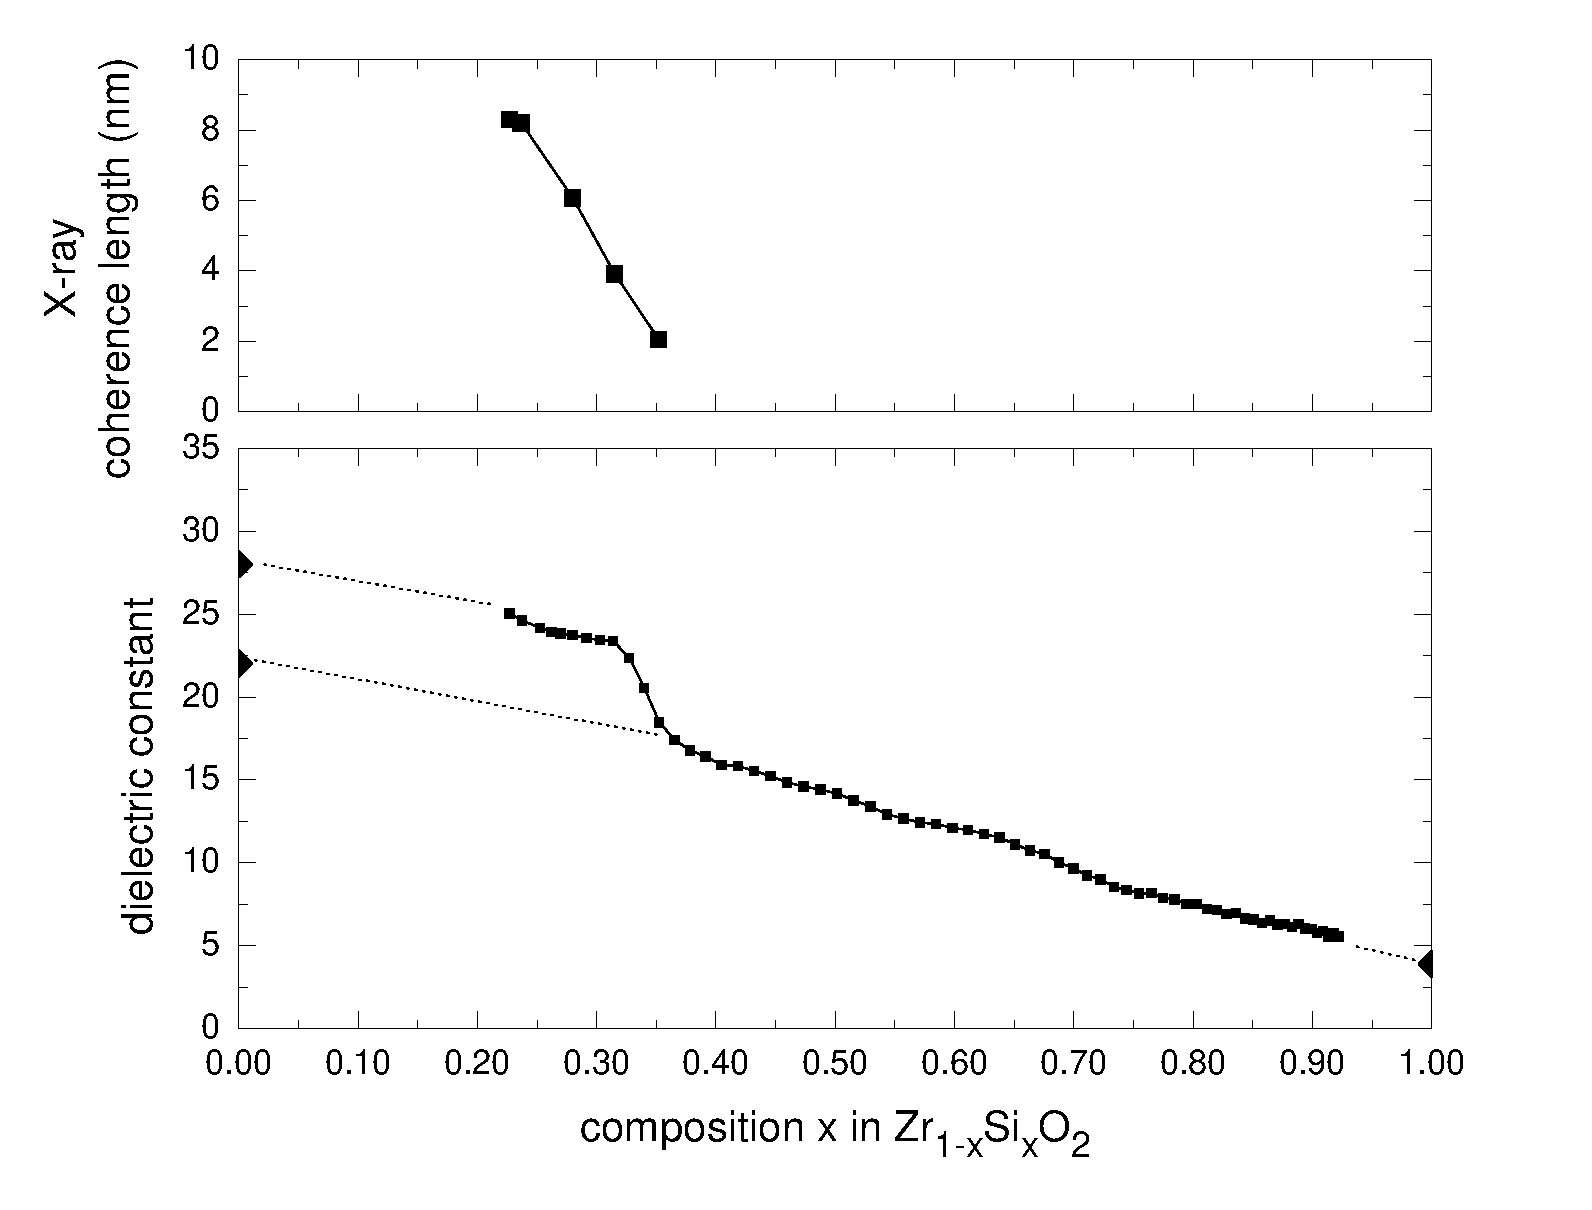
\includegraphics[width=\linewidth]{chapter_3/ZrSiO_epsilon_coherence.pdf}
\caption{Bottom: Composition dependence of the dielectric constant of thin film $\textnormal{Zr}_{1-x}\textnormal{Si}_{x}\textnormal{O}_{2}$ deposited at room temperature. Dotted lines represent extrapolations to values for the endmembers (crystalline and amorphous \ce{ZrO2} and amorphous \ce{SiO2}) indicated with triangles.Top: composition dependence of the structural coherence length (i.e., essentially grain size) as inferred from X-ray diffraction data using the Debye-Scherrer formula.}
\label{ZrSiO_eps_cohere}
\end{figure}

The major trend in dielectric constant as a function of composition in these systems is undoubtedly due to a change in the polarizability from the small values associated with \ce{SiO2} or \ce{Al2O3} to the large value associated with \ce{ZrO2}.  
But it is not immediately evident what fraction of the low-frequency polarizability can be attributed to ionic motion as opposed to polarization of the electrons with respect to atom cores, nor to what degree the density of the film plays a role. 
Fig. \ref{ZrAlO_ZrSiO_index} presents the composition dependence of the index of refraction in these systems. 
The data for $\textnormal{Zr}_{1-x}\textnormal{Al}_{x}\textnormal{O}_{2-x/2}$ follow a smooth trend that extrapolates almost linearly to accepted values for the endmembers \cite{Zhao2002,Kijima2000}.
The data for $\textnormal{Zr}_{1-x}\textnormal{Si}_{x}\textnormal{O}_{2}$ exhibits a more dramatic variation, extrapolating linearly to the endmember value for amorphous \ce{SiO2}. The data are insufficient to allow unambiguous extrapolation to \ce{ZrO2}, though they are consistent with the same value as inferred for $\textnormal{Zr}_{1-x}\textnormal{Al}_{x}\textnormal{O}_{2-x/2}$. 
Where the data for Zr-Al-O show only a break in slope associated with the crystalline-amorphous transition, the data for Zr-Si-O exhibit a jump similar to that observed in the static dielectric constant.    
%
\begin{figure}
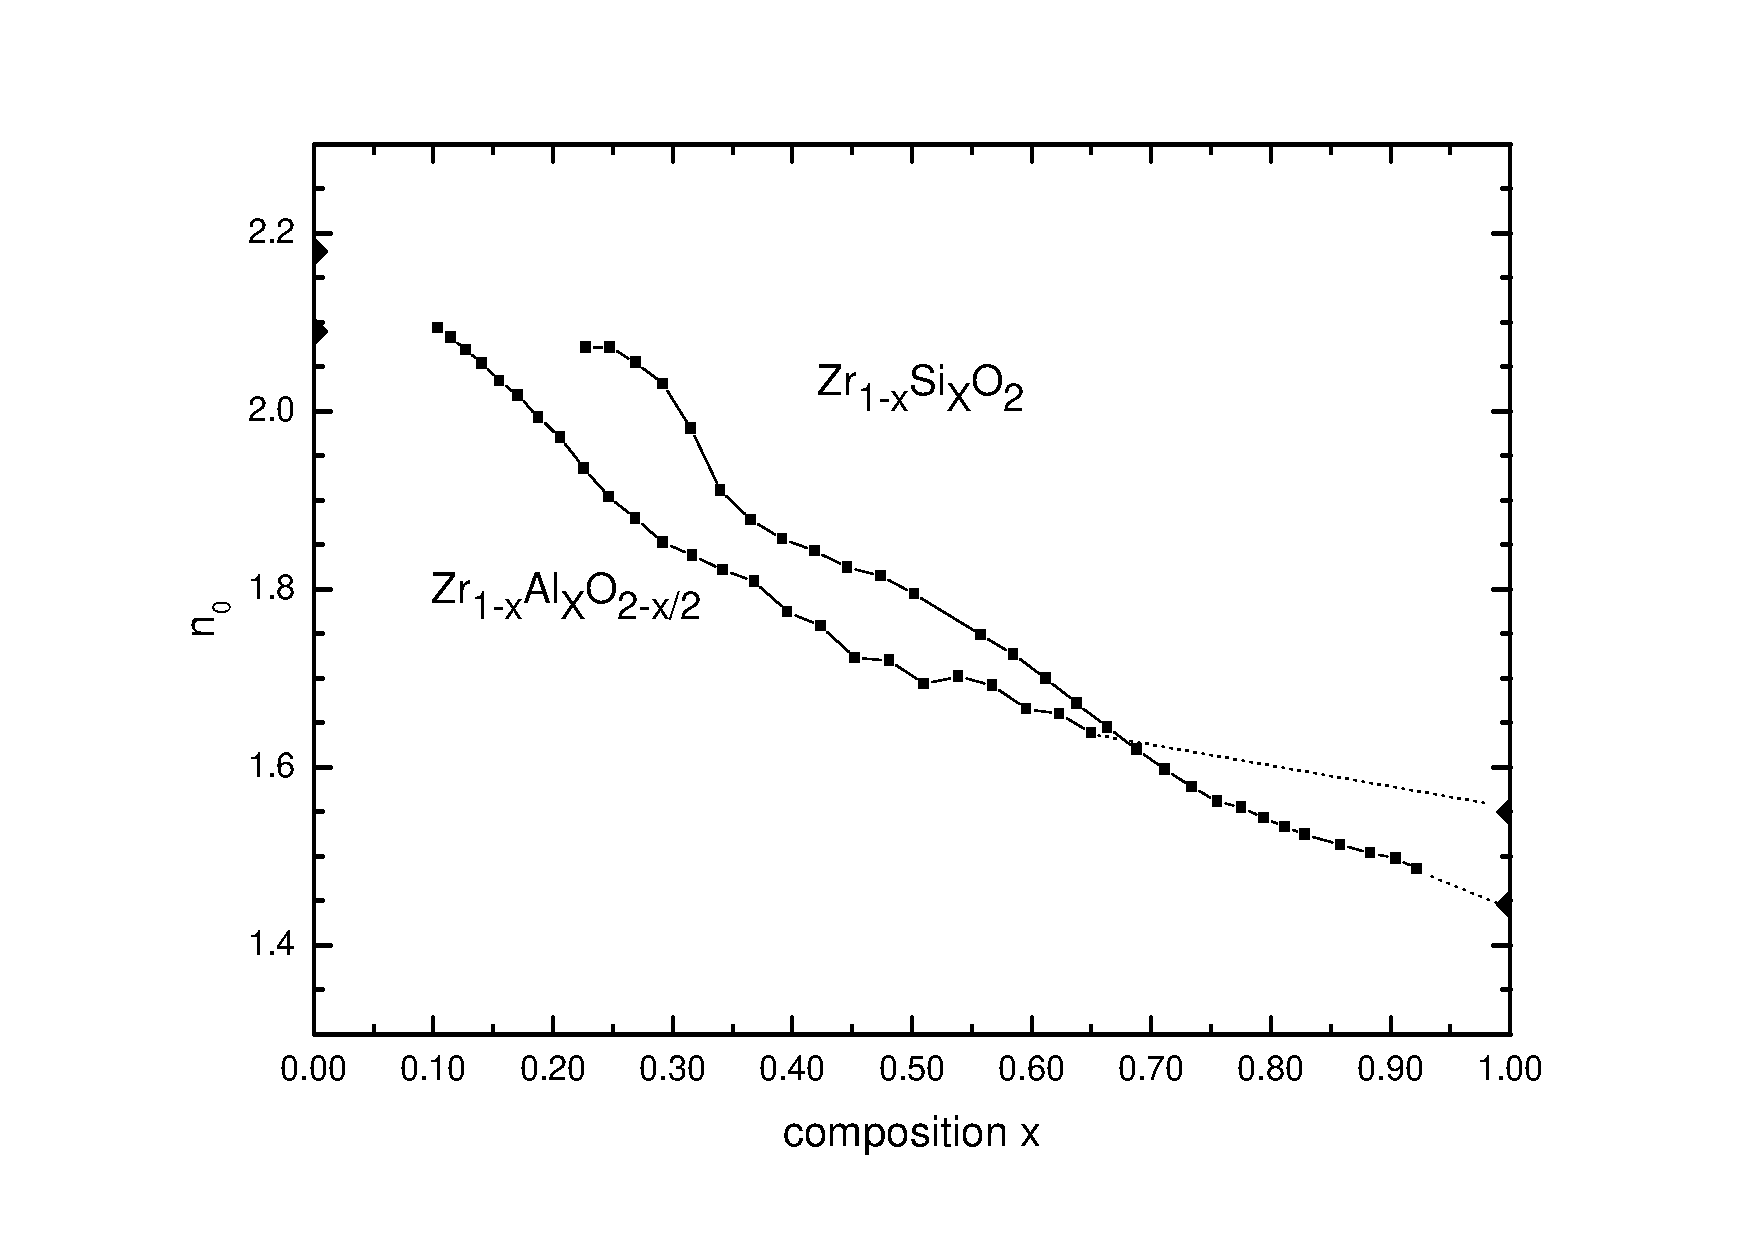
\includegraphics[width=\linewidth]{chapter_3/ZrAlO_ZrSiO_index.pdf}
\caption{Bottom: Composition dependence of the refractive index $n_0$ of thin film
$\textnormal{Zr}_{1-x}\textnormal{Al}_{x}\textnormal{O}_{2-x/2}$ and
$\textnormal{Zr}_{x}\textnormal{Si}_{1-x}\textnormal{O}_{2}$ 
deposited at room temperature. Dotted lines represent extrapolations to values for the endmembers (crystalline and amorphous \ce{ZrO2} and amorphous \ce{SiO2} and \ce{Al2O3}) indicated with triangles.}
\label{ZrAlO_ZrSiO_index}
\end{figure}
%
\subsection{Microscopic picture: static and electronic polarizability}
The high frequency dielectric constant is simply $\varepsilon_{\infty} = n^2$. See supplementary material at [URL will be inserted by AIP] for graphs comparing composition dependence of the static dielectric constant with the $\varepsilon_\infty$. 
But comparing $\varepsilon_s$ with $\varepsilon_{\infty}$ does not offer insight into the behavior at the local level because it does not account for depolarization effects and therefore does not account for density variations correctly. 
Interpreting local polarization behavior in this context does not mean associating a fixed polarizability with specific ions, but is simply a way to compare trends. 
A baseline expectation might be that the composition dependence of the polarizability interpolates linearly between the values for the endmembers. 
Deviations from that trend would suggest unexpected interactions or structural anomalies.

The Clausius-Mossotti equation relates the local polarizability to the externally observed dielectric constant:
$$
\frac{\varepsilon_s -1}{\varepsilon_s +2} = \frac{4 \pi}{3} \sum_{m}{\frac{\alpha_j}{V_m}}
$$
where $\alpha_j$ is the polarizability due to mechanism ${j \in \{electronic, ionic, dipolar, \ldots\}}$,
and $V_m$ is the molar volume.
For the materials under consideration only electronic ($\alpha_e$) and ionic ($\alpha_{ion}$) mechanisms are present. At optical frequencies, well above any phonon modes, only the electronic mechanism is active, so we can infer $\alpha_e /V$ directly from the refractive index. These values are plotted in Figs. \ref{ZrSiO_polariz_over_mol_vol} and \ref{ZrAlO_static_optical_polarizability}, for Zr-Si-O and Zr-Al-O, respectively. 

The data for \ce{SiO2}-rich Zr-Si-O closely follow a simple linear interpolation between the values for the endmembers; the slight deviations are not thought to be meaningful. For  $x < 0.35$ the deviation is significant and is associated with the presence of nanocrystallity. The data for $0.20 < x < 0.30$ are nearly constant, and match the value for unsubstituted \ce{ZrO2}.  We speculate that introduction of \ce{SiO2} decreases the polarizability and the molar volume at compensating rates, leaving $\alpha_e /V$ constant, and that at $x \approx 0.35$ the transition to a disordered structure leads to a fairly abrupt decrease in the molar volume.

The optical polarizability in the Zr-Al-O system follows a significantly different pattern. Here the trend deviates \emph{below} the linear interpolation of endmember values, suggesting either an increased molar volume or an electronic interaction that lowers the polarizability of the system. The data follow a relative smooth curve and extrapolate accurately to the values for the endmembers. In the Zr-Al-O system there is no abrupt transition in $\alpha_e$ associated with the crystalline-amorphous structural transition.     
%
\begin{figure}
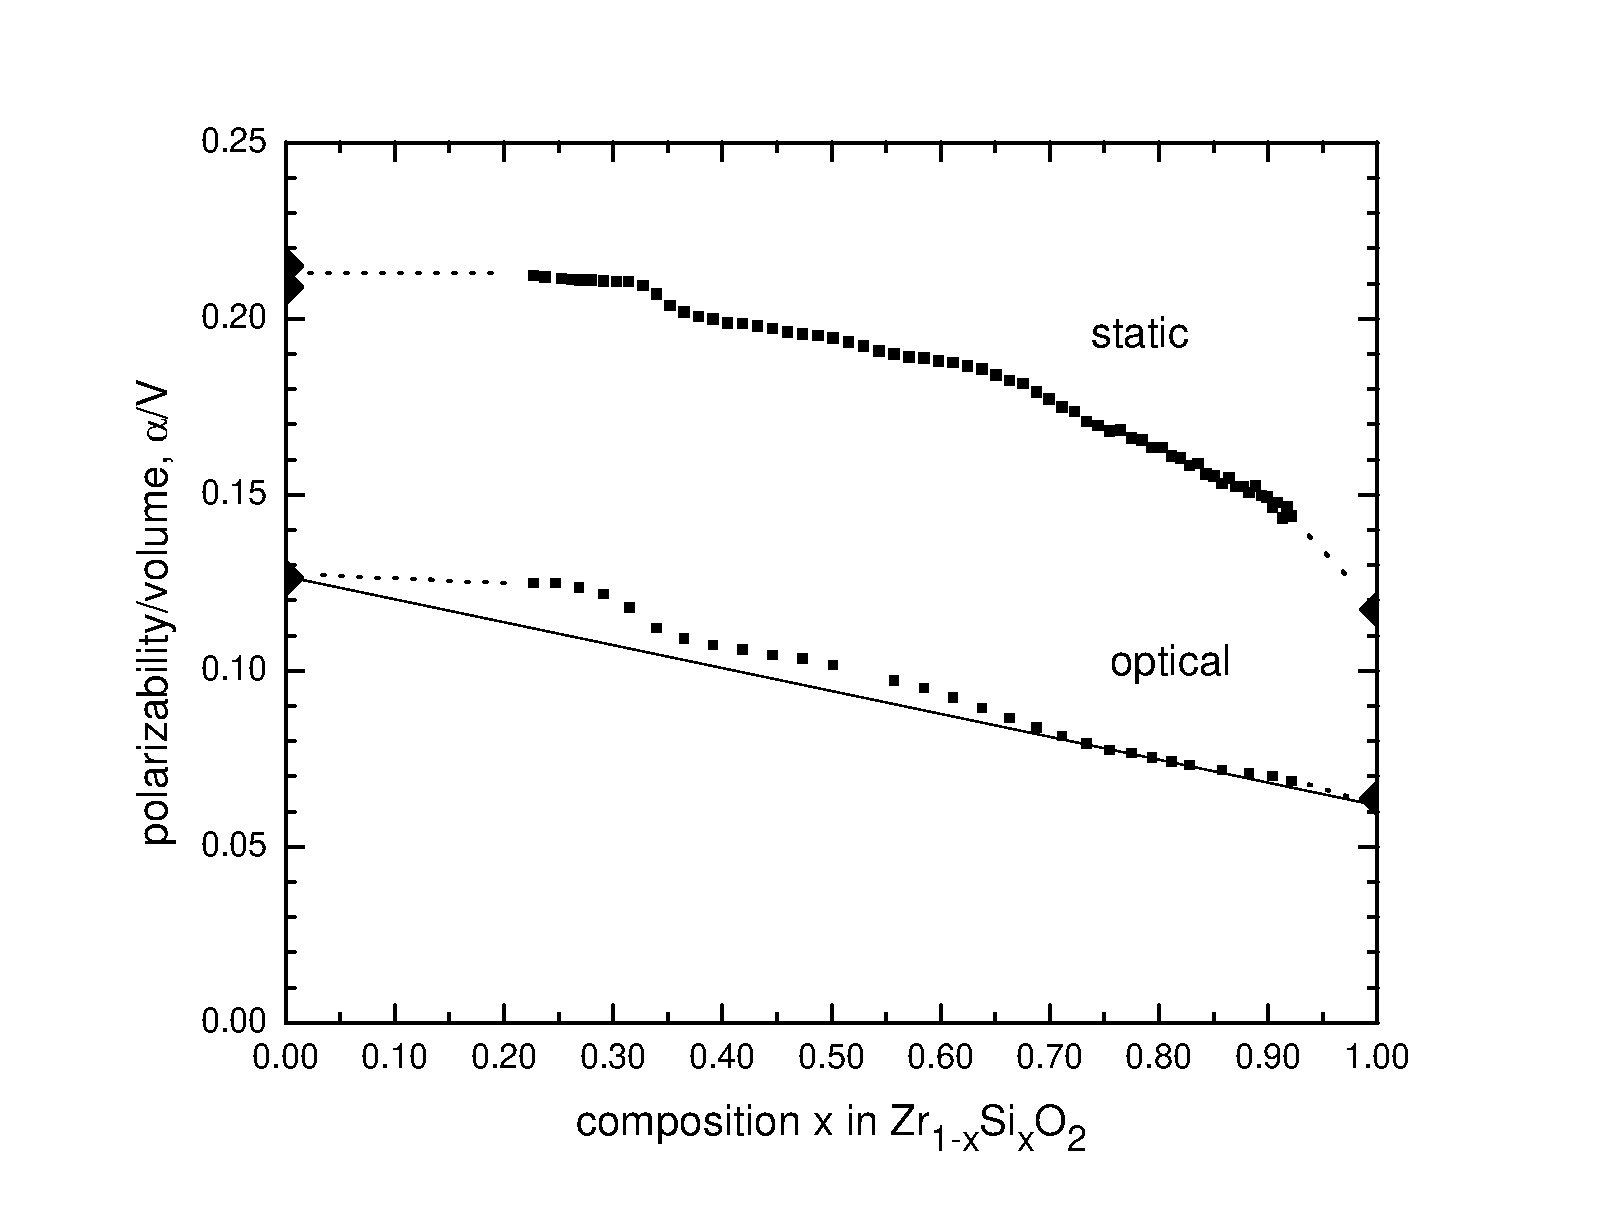
\includegraphics[width=\linewidth]{chapter_3/ZrSiO_polariz_over_mol_vol.pdf}
\caption{Composition dependence of the polarizability per unit volume, $\alpha /V$. Dotted lines are extrapolations to values for the endmembers (crystalline and amorphous \ce{ZrO2} and amorphous \ce{SiO2}) indicated with triangles. Top curve: polarizability inferred from the static (10 kHz) dielectric constant. Bottom curve: polarizability inferred from the optical index of refraction. The solid line is a simple interpolation between the values for the endmembers.}
\label{ZrSiO_polariz_over_mol_vol}
\end{figure}


Figures \ref{ZrSiO_polariz_over_mol_vol} and \ref{ZrAlO_static_optical_polarizability} also show the composition dependence of the static polarizability, $\alpha_s /V$, to which both electronic and ionic mechanisms contribute. In the $\textnormal{Zr}_{1-x}\textnormal{Si}_{x}\textnormal{O}_{2}$ system, $\alpha_s /V$ is nearly constant with increasing \ce{SiO2} fraction until at the crystalline/amorphous there is an abrupt decrease, presumably associated with an increase in molar volume. For $x > 0.35$ the trend of $\alpha_s (x)/V$ shows clear negative curvature, leading to a rapid decrease for the most \ce{SiO2}-rich compositions. In the $\textnormal{Zr}_{1-x}\textnormal{Al}_{x}\textnormal{O}_{2-x/2}$ system a less pronounced decrease is associated with the crystalline/amorphous transition, and there is almost no curvature in $\alpha_s (x)/V$ for $x > 0.35$. Fairly abrupt transitions in both the optical and static polarizability are seen around $x = 0.3$ for both chemical systems, clearly associated with the transitions in the dielectric constant. These might be related to changes in molecular density, or could indicate a change in one of the mechanisms for the polarizability.
%
\begin{figure}
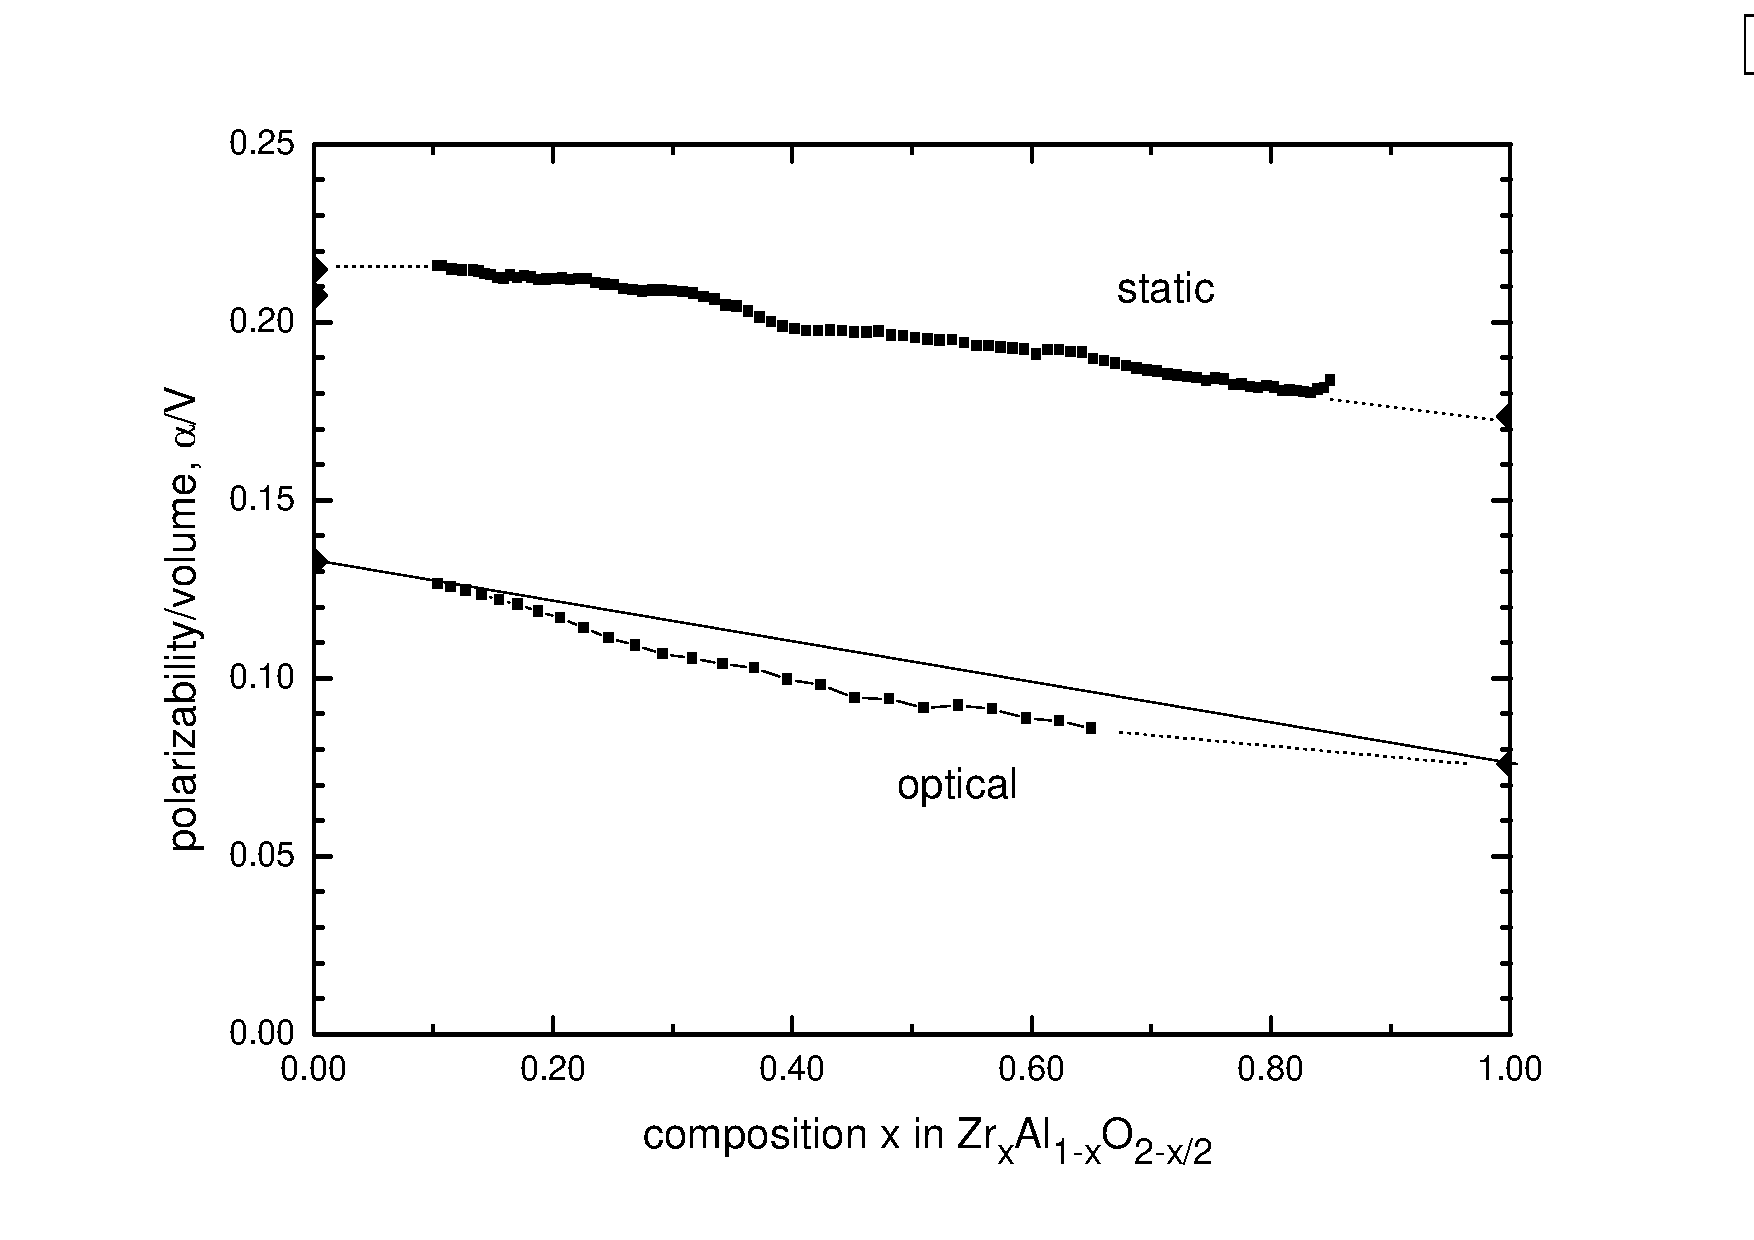
\includegraphics[width=\linewidth]{chapter_3/ZrAlO_static_optical_polarizability.pdf}
\caption{Composition dependence of the polarizability per unit volume, $\alpha /V$. Dotted lines are extrapolations to values for the endmembers (crystalline and amorphous \ce{ZrO2} and amorphous \ce{Al2O3}) indicated with triangles. Top curve: polarizability inferred from the static (10 kHz) dielectric constant. Bottom curve: polarizability inferred from the optical index of refraction. The solid line is a simple interpolation between the values for the endmembers.}
\label{ZrAlO_static_optical_polarizability}
\end{figure}
%
\subsection{Microscopic picture: ionic polarizability}
The difference between the static and optical dielectric responses is due to the displacement of ions, a mechanism that is active only at phonon frequencies and below. Thus the ionic contribution can be inferred using $\alpha_{ionic} /V = \alpha_s /V - \alpha_e /V$. In Fig. \ref{ZrSiO_ZrAlO_diff_polariz} we calculate this difference using the data of Figs. \ref{ZrSiO_polariz_over_mol_vol} and \ref{ZrAlO_static_optical_polarizability}, in which the optical polarizability was interpolated using a cubic spline before subtracting from the static polarizability. Although the data exhibit small wiggles that are probably not meaningful, the two systems demonstrate clearly different trends. The data for both compositions spreads can be seen to extrapolate plausibly to standard values inferred for the endmembers. The Zr-Al-O system exhibits a distinct increase in $\alpha_{ionic} /V (x)$ for increasing $x$ up to $x \approx 0.3 $, after which $\alpha_{ionic} /V$ is nearly independent of $x$. The Zr-Si-O system shows almost the opposite trend: a roughly constant value for $\alpha_{ionic} (x) /V$ for $x < 0.7$ followed by a rapid decrease as the \ce{SiO2} is increased further.
 
At $x = 0.3$, the data $\alpha_{ionic}(x) /V$ in Zr-Al-O do not exhibit a transition comparable to that seen in $\alpha_{e}(x) /V$; only a modest change of overall slope is observed. If the transition in $\alpha_{e}(x) V$ were due to a change in molecular volume $V$, a comparable transition should be observed $\alpha_{ionic}(x) /V$. 
The lack of such a feature implies that the change is in the polarizability $\alpha_e(x)$ at the crystalline/amorphous transition is due to a reorganization of the electron density in the system. 
By comparison, the data for Zr-Si-O are consistent with a model in which the transition is due to a change in molecular volume $V$ rather than $\alpha_{ionic}$ or $\alpha_e$. 

The composition dependence of the dielectric properties of Zr-Al-O and Zr-Si-O follow trends that are subtly but profoundly different, though this is not readily apparent in observations of only the static dielectric constant. 
The main differences are ascribed to substantial changes in bonding and ion dynamics associated with incorporation of \ce{ZrO2} in amorphous \ce{SiO2}-rich Zr-Si-O and incorporation of \ce{Al2O3} in \ce{ZrO2}-rich Zr-Al-O 
(but not with incorporation of \ce{SiO2} in \ce{ZrO2}-rich Zr-Si-O or incorporation of \ce{ZrO2} in amorphous \ce{Al2O3}-rich Zr-Al-O). 
We suggest that this reflects, in the first case, the difference in oxygen coordination for Si (typically tetrahedral) compared to that for Zr (typically octahedral). 
In the second case, it may also reflect the different valence of Al (typically 3$^+$) compared to that of Zr (typically 4$^+$), which would introduce oxygen vacancies to maintain charge neutrality.
The role played by changes in molar volume are not determined in this study, but we speculate that the overall smooth trend in enhancement of the ionic polarizability in Zr-Al-O may be attributed to modest changes in molar volume.
The abrupt change in the polarizability in Zr-Si-O at $\approx$35\% Si can plausibly be attributed to a change in molar volume associated with the crystalline/amorphous transition.
A more conclusive interpretation of the bonding changes would require data from local probes such as EXAFS, or Raman or infrared spectroscopy, coupled with \textit{ab initio} calculations of average structure in the amorphous materials.              
%
\begin{figure}
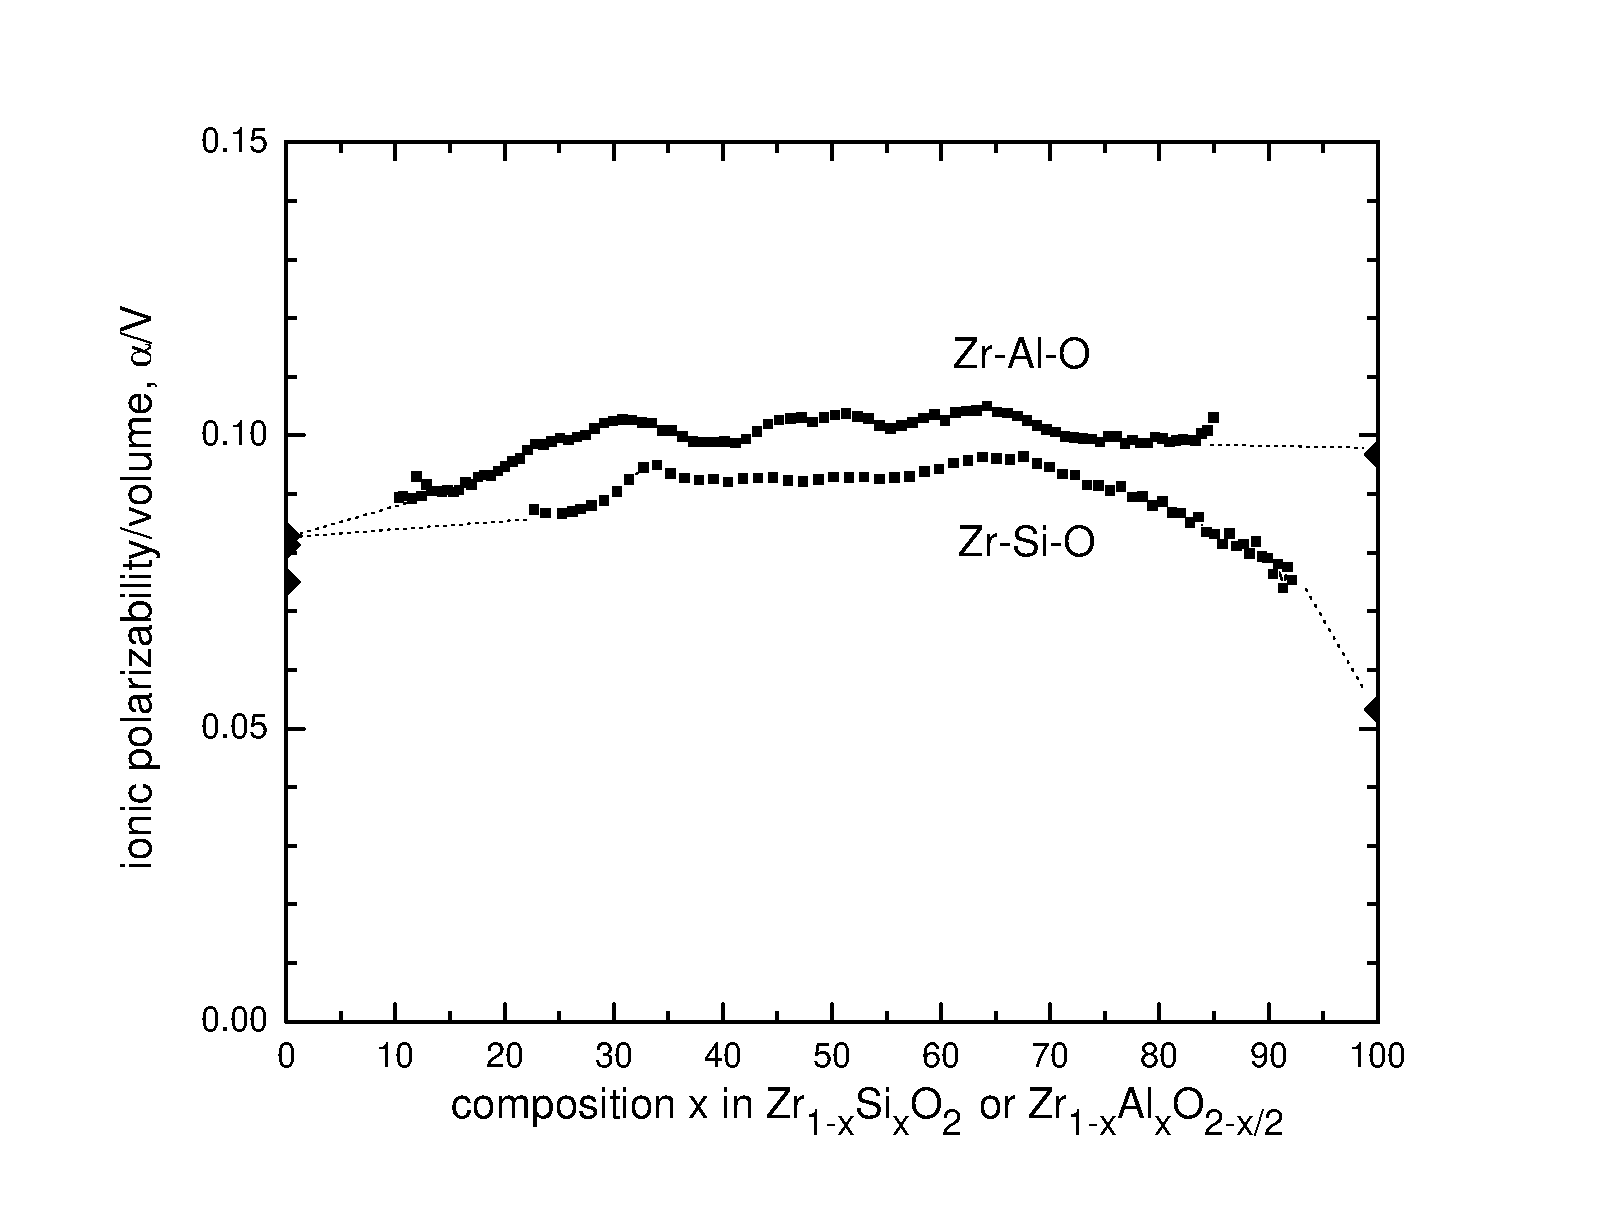
\includegraphics[width=\linewidth]{chapter_3/ZrSiO_ZrAlO_diff_polariz.pdf}
\caption{Composition dependence of the ionic polarizability,, as inferred from the text. Dotted lines represent extrapolations to values for the endmembers (crystalline and amorphous \ce{ZrO2} and amorphous \ce{SiO2} and \ce{Al2O3}) indicated with triangles.} 
\label{ZrSiO_ZrAlO_diff_polariz}
\end{figure}

\subsection{Breakdown field}
The leakage current and breakdown field of these materials is of significant technological interest, as they affect their suitability for any application in which charge or energy storage is important. 
Both properties depend on extrinsic mechanism such as details of impurity concentration, local inhomogeneity, film smoothness, electrode composition, etc., so that few general conclusions can be drawn. 
Fig. \ref{ZrSiAlO_Ebreakdown} presents composition dependence of the breakdown field for $\textnormal{Zr}_{1-x}\textnormal{Al}_{x}\textnormal{O}_{2-x/2}$ and $\textnormal{Zr}_{1-x}\textnormal{Si}_{x}\textnormal{O}_{2}$. For both materials, the breakdown fields range from $\approx 4$ MV/cm for the Zr-rich compositions to $\approx 6$ MV/cm for the Al-rich and Si-rich compositions. 
The significant feature in this data is that in both systems there is no change in breakdown field associated with the crystalline/amorphous transition at $x \approx 0.35$. 
This result clearly repudiates the conventional wisdom that the breakdown field of thin film polycrystalline materials must be compromised due to ``weak'' grain boundaries, as is observed in bulk ceramics. 
As indicated by the crystallite size plotted in Figs. \ref{ZrAlO_epsilon_cohere} and \ref{ZrSiO_eps_cohere}, the films have a high density of grain boundaries. 
This behavior suggests that grain boundaries in the thin films do not act as sinks for impurities and defects during growth, unlike those in high-temperature processed bulk ceramics.       
%
\begin{figure}
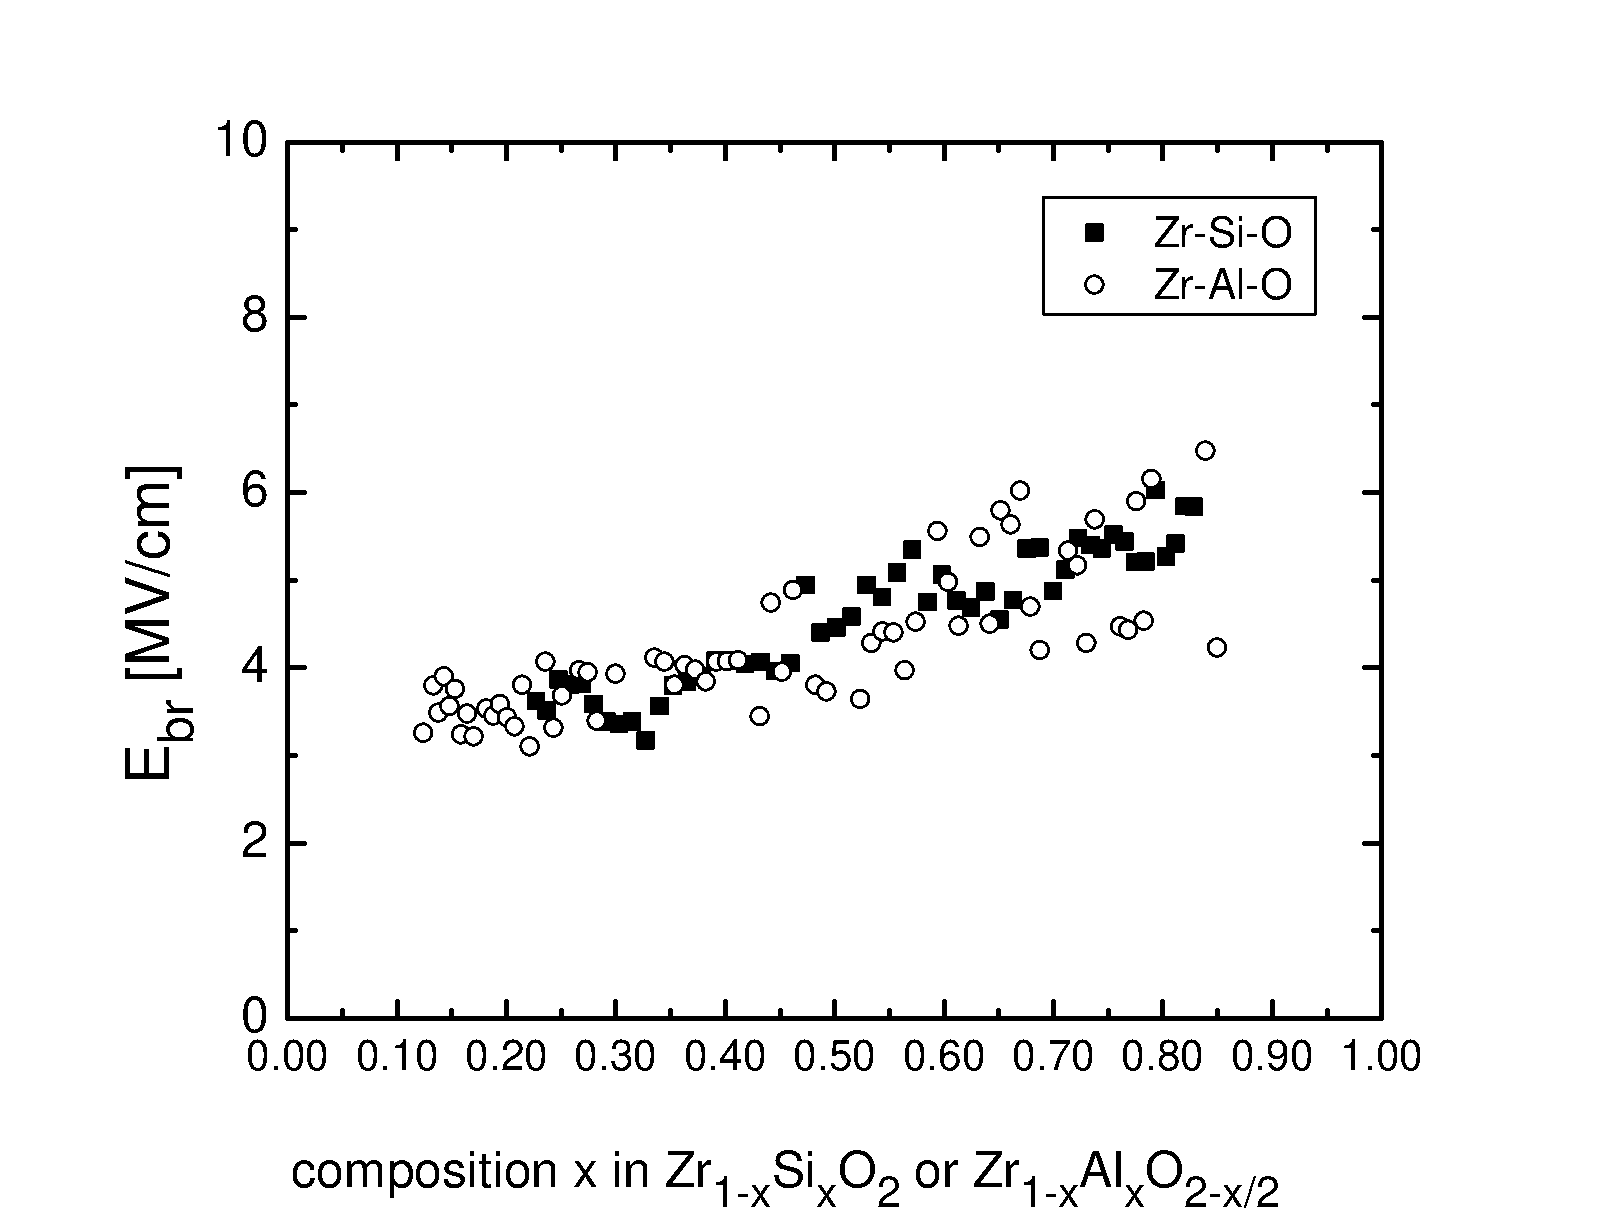
\includegraphics[width=\linewidth]{chapter_3/ZrSiAlO_Ebreakdown.pdf}
\caption{Composition dependence of the breakdown field in Zr-Si-O and Zr-Al-O. Solid symbols represent Zr-Al-O capacitors and open circles represent Zr-Si-O capacitors. Notice that no change in the trend is associated with the crystalline/amorphous transition at $x \approx 0.35$.}
\label{ZrSiAlO_Ebreakdown}
\end{figure}

\section{Conclusion}

This work shows that thin films of mixed transition-metal/p-block oxides, such as Zr-Si-O, are not as simple as they appear at first glance. Enhancement of the composition-dependent polarizability in amorphous \ce{SiO2}-rich Zr-Si-O is definitively confirmed in the data, while a comparable enhancement in \ce{Al2O3}-rich Zr-Al-O is ruled out though an enhanced polarizability in \ce{ZrO2}-rich Zr-Al-O is observed. 
In Zr-Si-O, but not Zr-Al-O, a change in molecular volume appears to be associated with the crystalline/amorphous transition. 
The changes in low-frequency polarizability are most plausibly attributed to changes in ion dynamics (phonon spectrum), suggesting further experiments directly probing the dynamics by IR spectroscopy. 
No significant change in the breakdown field associated with the crystalline vs. amorphous condition.     

\section{Acknowledgments}
This work was supported by the U.S. Department of Energy under Grant No. DE-FG02-06ER06-15. 
This work was performed in part at the Cornell NanoScale Facility, a member of the National Nanotechnology Infrastructure Network, which is supported by the National Science Foundation under Grant No. ECS-0335765. Additionally, this work made use of the Cornell Center for Materials Research facilities with support from the National Science Foundation Materials Research Science and Engineering Center program under Grant No. DMR-0520404. Preliminary data was obtained at Lucent Technologies Bell Labs. The authors thank Dr. R. M. Fleming for collecting and interpreting the RBS data.


% chapter 4
\chapter{Dielectric Properties of Amorphous Ta-Ge-O and Ta-Si-O Thin Films}

This chapter is adapted from T. A. Naoi and R. B. van Dover: ``Dielectric Properties of Amorphous Ta-Ge-O and Ta-Si-O Thin Films'' \emph{Journal of Applied Physics}.


% chapter 5
\chapter{Atomic structure determination of mixed amorphous Ta$_{2}$O$_{5}$-GeO$_{2}$ thin films deposited on silicon nitride membranes}

{\let\thefootnote\relax\footnote{{
This chapter is adapted from T. A. Naoi, S. J. Honrao, L. W. Taylor, D. S. Dale, R. G. Hennig, and R. B. van Dover: ``Atomic structure determination of mixed amorphous Ta$_{2}$O$_{5}$-GeO$_{2}$ thin films deposited on silicon nitride membranes.'' Manuscript in preparation.
}}}

% ABSTRACT
\section{Abstract}
We have probed the local structure of amorphous Ta$_{x}$Ge$_{1-x}$O$_{2+x/2}$ thin films over a range of compositions (including binary Ta$_{2}$O$_{5}$) using x-ray diffraction, x-ray absorption spectroscopy, and \emph{ab-initio} molecular dynamics. The films were sputtered on thin silicon nitride windows to minimize scattering from the underlying substrate, greatly facilitating the background subtraction process. Coordination numbers and bond distances for pure amorphous Ta$_{2}$O$_{5}$ are similar to values reported in previous studies. Incorporation of GeO$_{2}$ in Ta$_{2}$O$_{5}$ results in substantial deviation in the local environments compared to those of pure Ta$_{2}$O$_{5}$. The suppression in density reported previously for Ta-rich Ta$_{x}$Ge$_{1-x}$O$_{2+x/2}$ is attributed to an increase in bond distances, while the enhancement of the dielectric constant is linked to changes in local coordination.
    
\section{Introduction}
Ta$_{2}$O$_{5}$ is a dielectric that possesses many desirable properties and has been studied extensively \cite{Chaneliere1998}. Recently, it was observed that introducing a small amount of GeO$_{2}$ into amorphous Ta$_{2}$O$_{5}$ dramatically increases the dielectric constant of the material at low GeO$_{2}$ concentrations while retaining its amorphicity \cite{Naoi2012}, whereas SiO$_{2}$ substitution did not elicit this anomalous behavior \cite{Naoi2018jap}. Furthermore, changes in Ta/Ge composition were shown to greatly affect the Ta$_{x}$Ge$_{1-x}$O$_{2+x/2}$ density, one notable feature being the substantial suppression of the density below the linearly interpolated value for Ta-rich compositions. Again, Ta$_{x}$Si$_{1-x}$O$_{2+x/2}$ serves as a counterexample in that the density varies simply linearly with composition. The large discrepancy between the structure and dielectric properties of Ta$_{x}$Si$_{1-x}$O$_{2+x/2}$ and Ta$_{x}$Ge$_{1-x}$O$_{2+x/2}$ is surprising because SiO$_{2}$ and GeO$_{2}$ are chemically similar.

For crystalline mixtures, it is not surprising to find that mixing two or more dielectric materials would result in unusual dielectric properties. For example, alloying ZrO$_{2}$ with a small fraction of Y$_{2}$O$_{3}$ stabilizes the cubic zirconia phase, enhancing the dielectric constant to $\epsilon_r = 29$, compared to the dielectric constant of pure ZrO$_{2}$, $\epsilon_r = 22$ \cite{Subramanian1989}. Similarly, alloying Ta$_{2}$O$_{5}$ with TiO$_{2}$ results in a near fourfold increase in the dielectric constant \cite{Cava1995}. These dielectric anomalies are outstanding consequences of the link between changes in structure and dielectric behavior. In contrast, when the same materials are combined in amorphous form, enhancement is not typically observed \cite{Jeong2005, Gan1998, Fujikawa1994}. One might expect that a thin film chemical system that is amorphous for all compositions would yield structural and dielectric property trends comparable to those of the Ta$_{x}$Si$_{1-x}$O$_{2+x/2}$ system, \emph{i.e.}, in that these properties interpolate linearly with composition. Such an expectation is overly simplistic since it ignores the interplay of local bonding units (LBUs) at the atomic level and the ways in which local atomic configurations manifest in macroscopic properties. The complexity of the matter is exemplified in studies of amorphous zirconium and hafnium silicates \cite{Rignanese2002, Pignedoli2007}, which demonstrated that the dielectric properties in these amorphous systems are highly contingent on the stabilization of certain LBUs.

In this study, we systematically investigate the local structure of amorphous Ta$_{2}$O$_{5}$ and Ta$_{x}$Ge$_{1-x}$O$_{2+x/2}$ with the goal of relating previously reported macroscopic properties to local atomic configurations by simultaneously applying Pair Distribution Function (PDF) methods, x-ray absorption spectroscopy (XAS)---specifically Extended X-ray Absorption Fine Structure (EXAFS), and \emph{ab-initio} Molecular Dynamics (MD). Combining various complementary techniques greatly reduces the structure space that must be explored by constraining the structural parameters of the local environment. This is particularly important for complex amorphous materials because one cannot employ refinement techniques based on crystal symmetry. Deposition of thin films on nitride membrane arrays greatly facilitates the background subtraction of peaks caused by Si thermal diffuse scattering \cite{Gregoire2009a} and allows for multiple sample compositions to be probed from a film deposited in one experiment on a single Si substrate, thus avoiding sample-to-sample variation in deposition conditions.

\section{Experimental Details}
\subsection{Silicon nitride membrane fabrication and thin film deposition}  

%Si3N4 membrane fabrication in CNF 
Silicon nitride membrane arrays were fabricated using standard clean room processes in the Cornell Nanofabrication Facility. The membranes were arranged in a two-dimensional array as shown in Figure \ref{fig:mem}. Windows for the 12x12 array were 2 mm on a side, whereas the windows for the 8x8 arrays were 3 mm. Prior to silicon nitride deposition, 75 mm diameter double-side-polished Si wafers were cleaned in an acid bath followed by a base bath, rinsing in deionized water after each bath. The wafers were then transferred to an MRL Industries low pressure chemical vapor deposition (LPCVD) furnace where low stress silicon nitride was deposited. The silicon nitride deposition rate was approximately 3 nm/minute as determined in prior calibration runs. The substrates were maintained in the furnace for 7 hours at 775 \textdegree C, which yielded nitride films that were approximately 1.5-1.6 microns thick as determined by reflectometry (FilMetrics Film Measurement System). The window array patterns were developed on the wafer using standard photolithographic methods. This involves transferring a photoresist pattern of the array onto the nitride coated substrate and etching away the nitride in the exposed windows. Finally, the wafer was back-etched using a potassium hydroxide solution leaving intact silicon nitride windows.

%Deposition of Ta2O5 and TaGeOx thin films using sputtering 
\begin{figure}[ht]
\centering
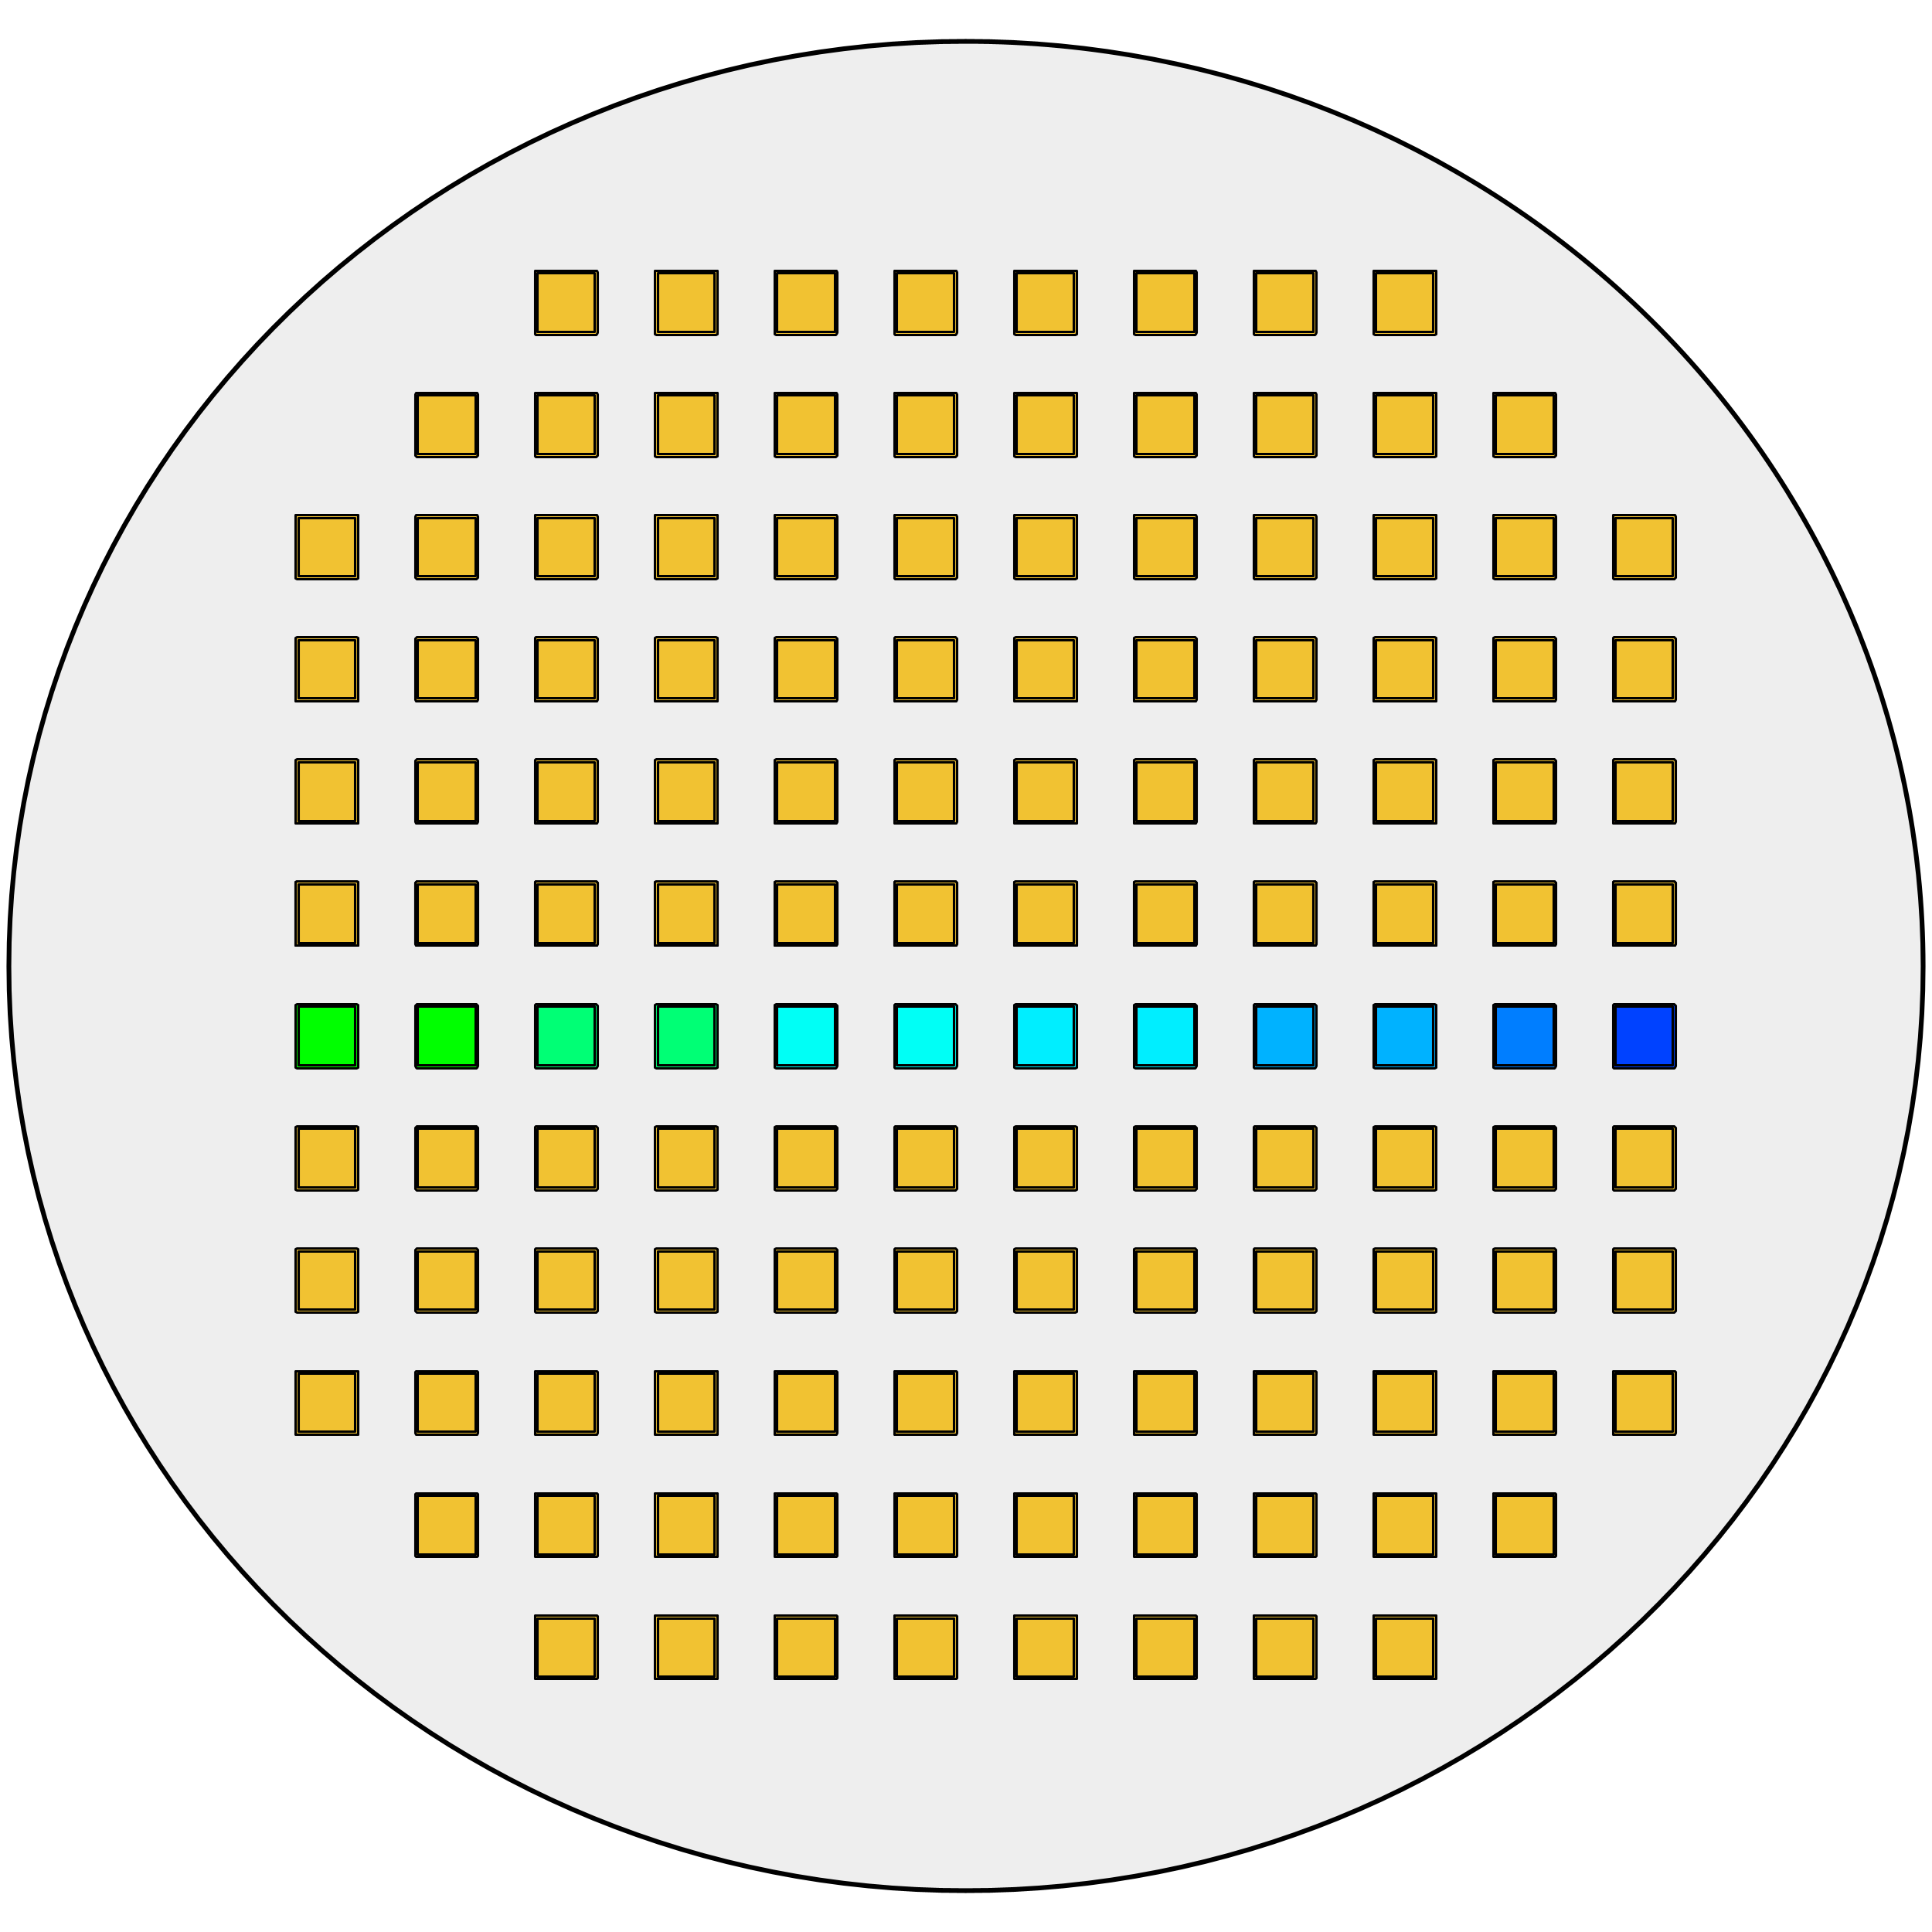
\includegraphics[width=0.5\textwidth]{./chapter_5/membranes.png}
\caption{A cartoon of the 12 $\times$ 12 silicon nitride membranes fabricated for the analysis of amorphous thin film oxides. This membrane shows a deposition of a binary composition spread indicated by the gradual color change of the center membranes. Blank membranes adjacent to the films were used for subtraction of the signal associated with the membrane itself.}
\label{fig:mem}
\end{figure}

Binary Ta$_{2}$O$_{5}$ and Ta$_{x}$Ge$_{1-x}$O$_{2+x/2}$ composition spreads were deposited on the membrane-array wafers using reactive radio frequency (rf) sputtering from two-inch-diameter metal targets in the 90\textdegree off-axis configuration \cite{VanDover1998}. 
12x12 arrays were used for the Ta$_{x}$Ge$_{1-x}$O$_{2+x/2}$ spread, while the 8x8 pattern was used for Ta$_{2}$O$_{5}$ since the latter film had no composition gradient. 
Parts of the wafer were covered with clean Si to mask deposition so that the Ta$_{x}$Ge$_{1-x}$O$_{2+x/2}$ film was deposited onto only a single row of membranes along the center of the wafer (Figure \ref{fig:mem}). The uncoated membranes immediately adjacent to the coated membranes were used for background subtraction. Prior to film deposition the chamber was evacuated to a pressure of 10$^{-6}$ Torr. The working pressure during deposition was maintained at 30 mTorr using a throttle valve. 
Gas flow rates during deposition were 15 standard cubic centimeters per minute (SCCM) Ar and 10 SCCM O$_{2}$. The rf guns were operated at 100 W Ta and 20 W Ge. The substrate was also intentionally biased at -75 V using a separate rf power source. The substrate temperature during deposition was maintained below 60 \textdegree C.

\subsection{Data collection and analysis} 
\subsubsection{Diffraction experiment and PDF analysis} 

Room temperature diffraction experiments were performed at the Cornell High Energy Synchrotron Source (CHESS) A2 line in transmission at 40 keV ($\lambda=0.030657$ nm). The samples were oriented such that the x-rays entered the membranes perpendicular to the film surface; the scattered beam was collected using a General Electric (GE) DXR-250 area detector. The sample-detector distance was 422 mm as determined using Si powder mounted at the same position as the sample. This corresponds to a $Q_{\text{max}}\sim 12\;\text{\AA}^{-1}$ ($Q = 4\pi \sin{\theta}/\lambda$). The collection of data at positions across the wafer was enabled by a translation stage. Careful wafer alignment avoided inadvertent scattering from the Si substrate. 

The 2D diffraction images were azimuthally integrated into 1D intensity ($I_{m}$) versus $Q$ patterns using Fit2D \cite{Hammersley1996, Hammersley1998}. ($I_{m}$) was normalized for incident flux (ion chamber counts), and the signal from the uncoated membranes as well as the dark image were subtracted from the measured intensity of the coated membranes. The 1D data was then sine Fourier transformed into PDFs using PDFgetX3 \cite{Juhas2013a}. The PDF, or $G(r)$ is defined as,  
\begin{equation}
G(r) = \frac{2}{\pi} \int_{Q_{min}}^{Q_{max}} Q[S(Q)-1]\sin{(Qr)}dQ
\label{eq:sinetransform}
\end{equation}
\noindent where $S(Q)$ is the structure function. Integration of the Fourier kernel was carried out from $Q_{min} = 1$\;\AA$^{-1}$ to $Q_{max} = 11.7$\;\AA$^{-1}$ with an r$_{poly}$ of 1.33, where r$_{poly}$ is the data-correction polynomial. The composition associated with each PDF was determined using deposition rate profiles (estimated absolute error is less than 5 at\%; relative error is much lower).

\subsubsection{X-ray absorption spectroscopy} 

X-ray absorption spectra were collected simultaneously in transmission and fluorescent modes at the F3 line at CHESS. Samples were mounted on a linear translation stage, allowing for multiple sample runs on a single wafer minimizing sample disturbance. A standard double-crystal Si (111) monochromator was used to tune the energy of the x-ray beam to the Ta L$_{\text{III}}$ edge at 9881 eV. A metallic Ta film was used as a calibration sample. Absorption spectra were collected over the range of 9700-10900 eV for all samples.

Data from multiple sample runs were averaged and imported into Athena \cite{Ravel2005} for background subtraction and normalization to the edge step, where the edge energy was taken to be the maximum of the first derivative of the absorption. Energy shifts were applied to each sample based on the Ta calibration sample for energy grid calibration. $\chi(k)$ with a $k$ weight of two was then Fourier transformed into $R$-space by limiting the $k$-range from 2 to 11 \AA$^{-1}$ using a Kaiser-Bessel window.
The transformed data was then imported into Artemis \cite{Ravel2005}. Theoretical amorphous structures generated using \emph{ab-initio} MD were input into Artemis as Crystallization Information Files (CIFs), from which theoretical scattering pathways were calculated using FEFF6 \cite{Rehr2000}. The maximum cluster size in the FEFF calculation was limited to 10.0 \AA\, and the longest path to 5.0\,\AA. Theoretical scattering pathways were then used to fit the EXAFS spectra using the EXAFS equation:
\begin{equation}
\chi(k) = S^{2}_{0}\sum_{j}\frac{N_{j}f_{j}(k) e^{-2k^{2}\sigma_{j}^{2}} e^{-2R_{j}/\lambda(k)}}{2kR_{j}^{2}}\text{sin}[2kR_{j}+\delta_{j}(k)].
\label{eq:EXAFS}
\end{equation}
\noindent For each central absorbing atom, $N_{j}$ is the coordination number of the $j$th coordination shell, where the bond distance of the atom in the $j$th shell is indicated by $R_{j}$. $f_{j}(K)$ and $\delta_{j}(k)$ are values calculated \emph{ab-initio} and represent the scattering factor and phase shifts of the atoms in the $j$th coordination respectively. To account for thermal disorder of the system we include the $e^{-2k^{2}\sigma^{2}_{j}}$ term, in which $\sigma_{j}^{2}$ is the mean-squared displacement (MSD) of the bond distance $R$. Considerations for inelastic scattering of photo-electrons are contained in the $e^{-2R_{j}/\lambda(k)}$ term, with photoelectron mean free path $\lambda(k)$. Finally, the $S_{0}^{2}$ term is an amplitude reduction factor. The measured EXAFS is the sum of all the contributions from each scattering atom.

The general fitting strategy is to minimize the R-factor in Artemis through a least-squares regression, where a good fit is typically characterized by an R-factor $<$ 0.05. Variables allowed to float were the half-path length $R_{\Gamma}$, energy shift $\Delta E_{o}$, and mean-squared disorder $\sigma_{\Gamma}$. The amplitude, $S_{o}$, was generally set to a fixed value between 0.8 and 1.0 to evaluate the degeneracy of the coordination shell, $N_{\Gamma}$.

\subsubsection{Calculation details}

We employed a melt-and-quench approach \cite{PhysRevB.87.184114} using \emph{ab-initio} MD to generate amorphous structures. Using GASP, our genetic algorithm code for structure predictions \cite{0953-8984-25-49-495401}, we first created three random low-energy Ta$_{2}$O$_{5}$ amorphous structures (Ta$_{16}$O$_{40}$). These were heated past the melting point of Ta$_{2}$O$_{5}$ (up to 2500 K) and then cooled to room temperature. The structures were then relaxed to obtain the final approximates of the amorphous structure of Ta$_{2}$O$_{5}$. We used an energy convergence of 0.01 meV for self-consistency during the MD calculations and 0.001 meV for the final relaxations. A time step of 2 fs was used for all MD calculations. The temperature cycle for the melt-and-quench process is shown in Figure \ref{fig:quench}.

We also generated four Ta$_{x}$Ge$_{1-x}$O$_{2+x/2}$ compositions in addition to pure Ta$_{2}$O$_{5}$. Starting from the three previously generated amorphous structures, we replaced the required number of Ta atoms with Ge to obtain new structures at each of the following compositions: Ta$_{0.5}$Ge$_{0.5}$O$_{y}$ (Ta$_{8}$Ge$_{8}$O$_{40}$), Ta$_{0.75}$Ge$_{0.25}$O$_{y}$ (Ta$_{12}$Ge$_{4}$O$_{40}$), Ta$_{0.875}$Ge$_{0.1250}$O$_{y}$ (Ta$_{14}$Ge$_{2}$O$_{40}$), and Ta$_{0.9375}$Ge$_{0.06250}$O$_{y}$ (Ta$_{15}$Ge$_{1}$O$_{40}$). We performed the same melt-and-quench cycle on the new structures to obtain amorphous structures at all four compositions.

\begin{figure}[ht]
\centering
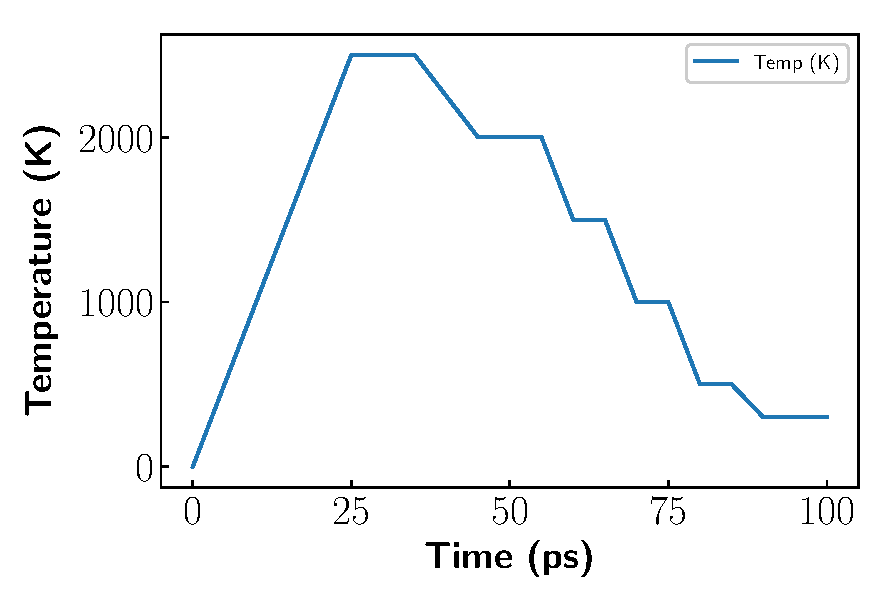
\includegraphics[width=0.6\textwidth]{./chapter_5/quench.eps}
\caption{Temperature cycle for the melt-quench process used to generate the amorphous structures.}
\label{fig:quench}
\end{figure}


\section{Results and Discussion} 
\subsection{Experimental PDFs for Ta$_{2}$O$_{5}$ and Ta$_{x}$Ge$_{1-x}$O$_{2+x/2}$}

The 2D background-subtracted diffraction image for Ta$_{2}$O$_{5}$ is shown in Figure \ref{fig:label:diff}. The broad circular rings in the diffraction image indicate that the film is amorphous as expected, since the crystallization temperature of Ta$_{2}$O$_{5}$ is high ($T_{cryst}\sim$ 650 \textdegree C) \cite{Joshi1999}. The images for Ta$_{x}$Ge$_{1-x}$O$_{2+x/2}$ (not shown) are visually very similar to the one in Figure \ref{fig:label:diff}, indicating that substitution by GeO$_{2}$ does not result in any detectable crystallization. We compare the 2D diffraction pattern in Figure \ref{fig:label:diff} with the azimuthally integrated diffraction pattern of Figure \ref{fig:label:ivq}. The abrupt decrease in the intensity for $Q<1$\;\AA\; is a simple artifact of the masking function applied in Fit2D to eliminate data where the detector is in the shadow of the beam stop.
\begin{figure}[ht]
\centering
\subfloat[\label{fig:label:diff}]{%
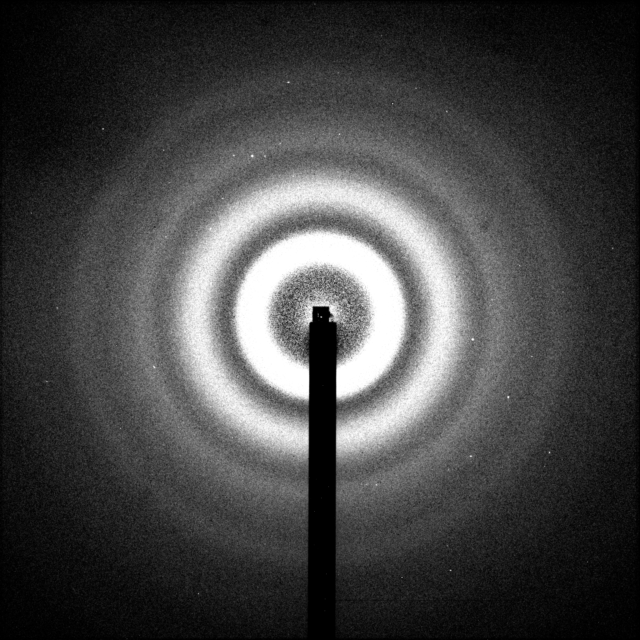
\includegraphics[width=0.4\textwidth]{./chapter_5/12F74-diff_640.png}}
\qquad
\subfloat[\label{fig:label:ivq}]{%
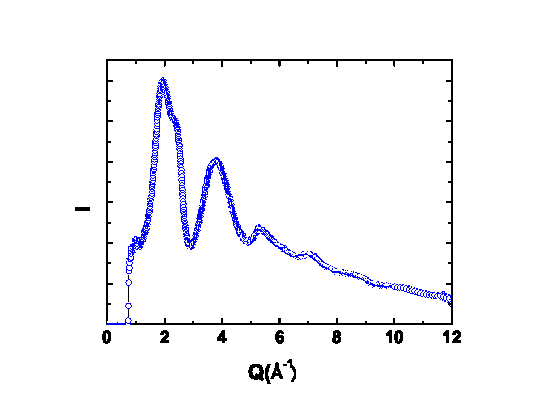
\includegraphics[width=0.6\textwidth]{./chapter_5/ivq.eps}}
\caption{(a) 2D diffraction image after background subtraction for pure Ta$_{2}$O$_{5}$ deposited on the silicon nitride membranes. 
(b) The resulting powder diffraction pattern after azimuthal integration of (a). 
The abrupt drop in the integrated intensity for low values of Q is a result of masking shadowed by the beam stop.} 
\label{fig:image}
\end{figure}

The PDF in Figure \ref{fig:grfq} displays a typical pattern generated using PDFgetX3 from the reduced structure function $F(\textbf{Q});$ the PDF shown is for amorphous Ta$_{2}$O$_{5}$. The series of PDFs for Ta$_{x}$Ge$_{1-x}$O$_{2+x/2}$ is displayed in the form of a waterfall and contour plot in Figure \ref{fig:pdf}. There is generally no discernible ordering in the PDF beyond 5\;\AA\, as demonstrated by the lack of peaks that exceed the noise. We determined the peak positions for each bond distance by fitting a Gaussian of the form,
\begin{equation}
\sqrt{\frac{2}{\pi}} \frac{A}{W}\exp\Big(\frac{-2(x-x_{c})^{2}}{W^{2}}\Big)
\label{eq:gauss}
\end{equation}
to each peak in the PDF. Here $A$, $W$, and $x_{c}$ are fitting parameters, and we take $x_{c}$ to be the center of the peak. Bond distances in the literature \cite{Bassiri2011, Solids1986, STONE2001769} served as a guide for peak identification. In pure Ta$_{2}$O$_{5}$ (Figure \ref{fig:grfq}), the peak located at roughly 1.9\;\AA\;is the Ta-O bond distance; we limited the fitting range to $r = 1.5-2.4$\;\AA\;to determine a precise bond distance of $r_{Ta-O}= 1.93$ \AA,\;which is comparable to reported bond distances \cite{Bassiri2011, Solids1986}. The smaller peak at $\sim$2.5\;\AA\; is the O-O pair distance; fitting a Gaussian over the range $r=2.4-2.85$\;\AA\; yields  $r_{O-O} = 2.47$ \AA. Finally, the peaks spanning from roughly $3-4$ \AA\ are attributed to Ta-Ta and Ta-O second neighbors.

Changes in the local environment of the material with substitution of GeO$_{2}$ into Ta$_{2}$O$_{5}$ are reflected by a shift in PDF peak positions (Figure \ref{fig:pdf}). Unfortunately, the resolution of the PDF limits our ability to properly attribute PDF peaks to Ta$_{2}$O$_{5}$ and GeO$_{2}$. For example, we expect a peak at around 1.73 \AA\;for the Ge-O pair \cite{STONE2001769} in the PDF pattern at 0.34 Ta cation fraction (Figure \ref{fig:pdf}), but we can only observe the peak at $\sim$1.85 \AA, which we presume contains overlapping Ta$_{2}$O$_{5}$ and GeO$_{2}$ peaks. As we alluded to earlier, we resolve the resolution problem by using EXAFS and \emph{ab-initio} MD data to supplement our results from the PDF analysis.

\begin{figure}[t]
\centering
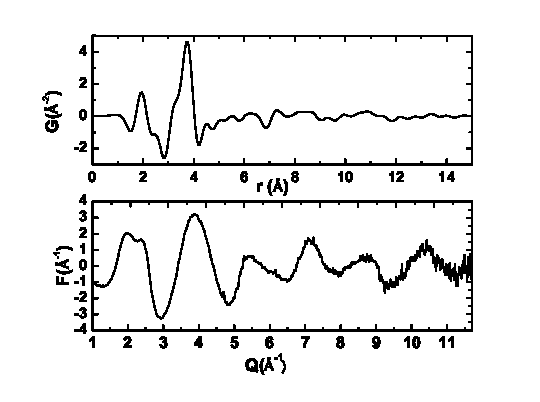
\includegraphics[width=0.8\linewidth]{./chapter_5/grfq.eps}
\caption{(Top) The generated PDF, G(r), calculated from the reduced structure function, F(Q), (Bottom) for pure Ta$_{2}$O$_{5}$.}
\label{fig:grfq}
\end{figure}

\begin{figure}[t]
\centering
\subfloat[\label{fig:label:waterfall}]{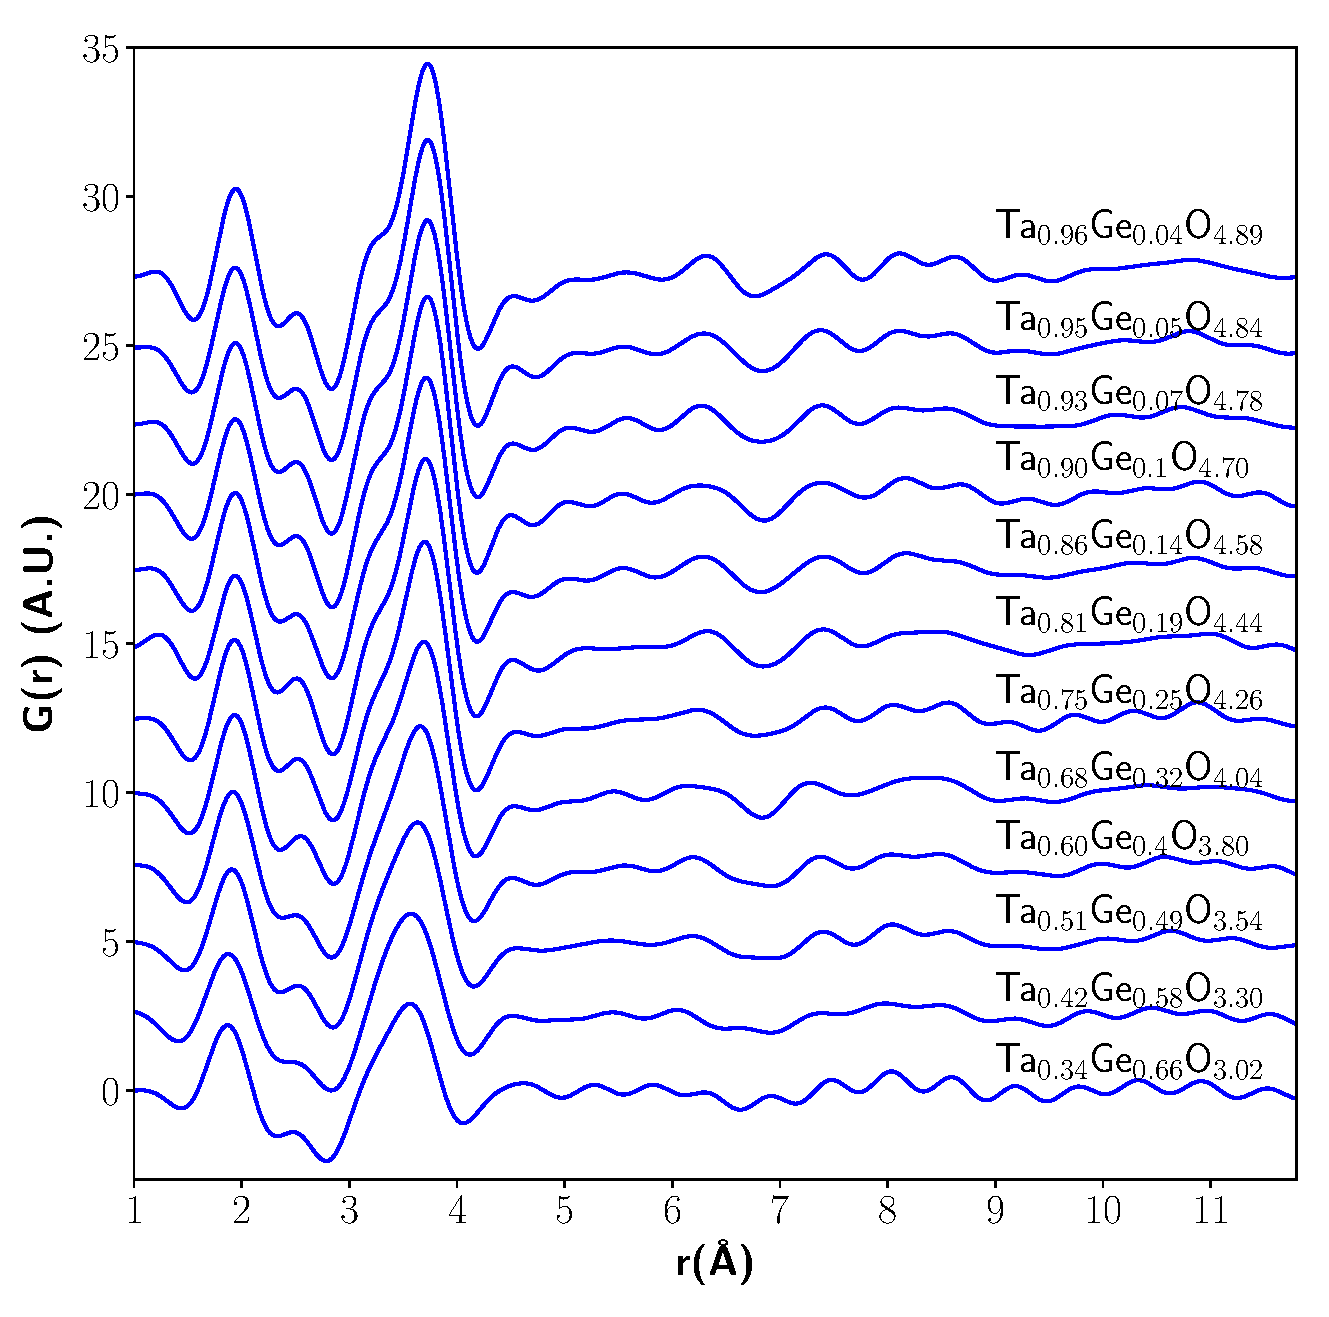
\includegraphics[width=0.5\textwidth]{./chapter_5/waterfall.eps}}
\qquad
\subfloat[\label{fig:label:contour}]{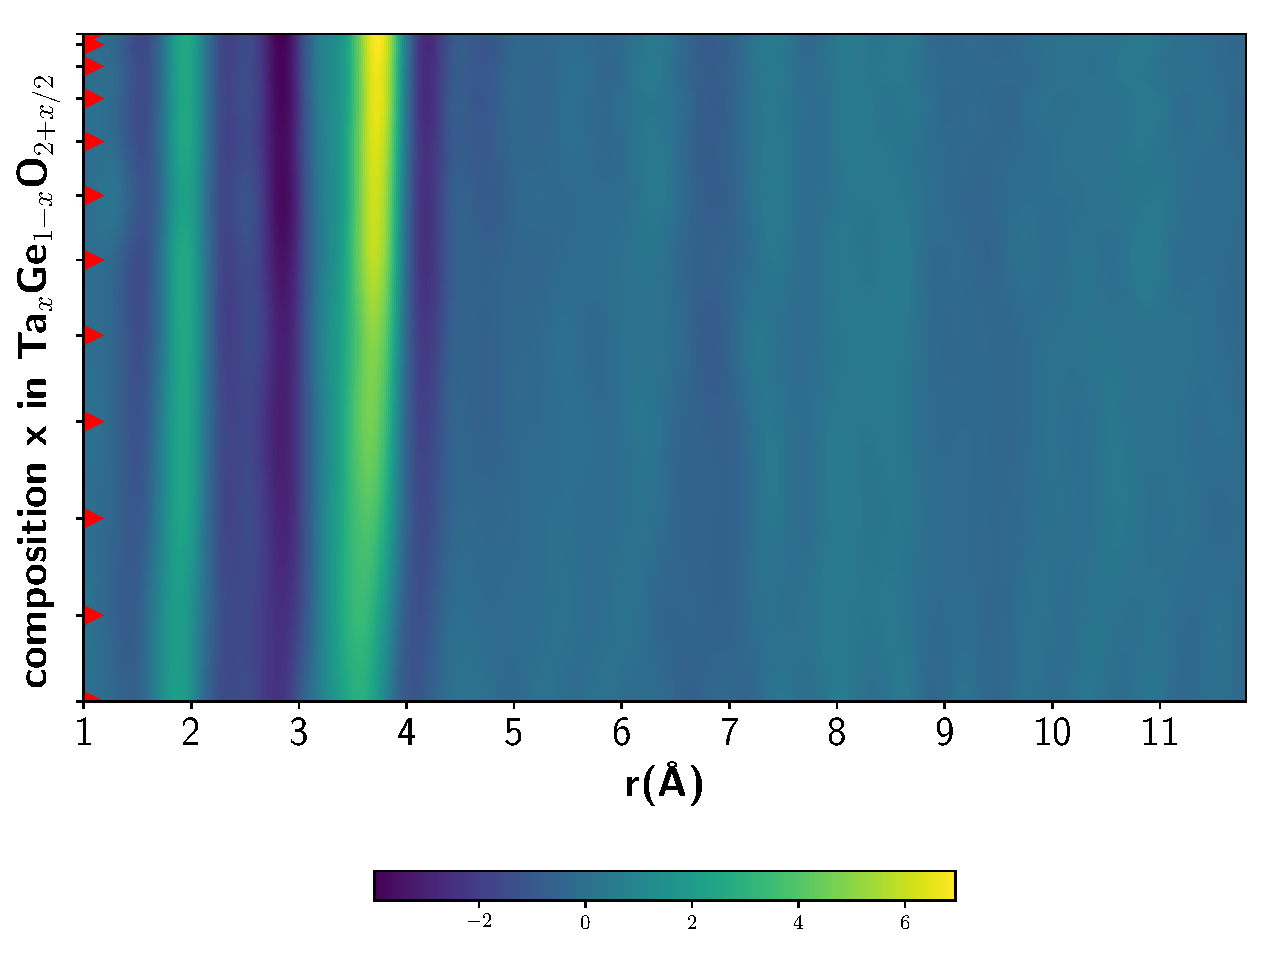
\includegraphics[width=0.6\linewidth]{./chapter_5/contour.eps}}
\caption{(a) Waterfall plot of the PDFs generated using PDFgetX3 for Ta$_{x}$Ge$_{1-x}$O$_{2+x/2}$ compositions. The Ta cation composition $x$, increases from bottom to top. (b) A heatmap plot of the same set of PDFs as in (a). The color scale plot corresponds to the height of the PDF. Red arrows on the y-axis mark the specific compositions measured, while the compositions in between are algorithmically interpolated.}
\label{fig:pdf}
\end{figure} 

\subsection{Uncovering structural trends of Ta$_{x}$Ge$_{1-x}$O$_{2+x/2}$ using EXAFS and PDF data}

\begin{figure*}[ht]
\centering
	\subfloat[\label{fig:label:xas_mu}]{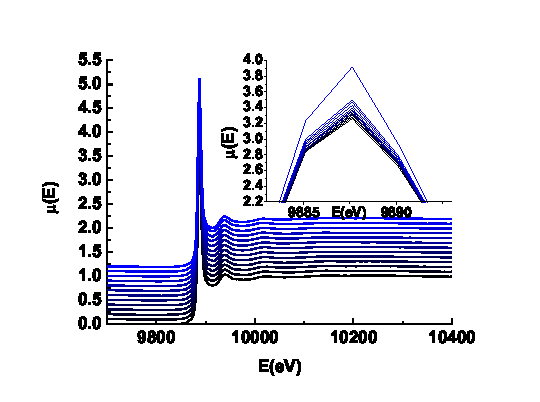
\includegraphics[width=0.5\textwidth]{./chapter_5/xas_mu.eps}}
	\hspace{-1ex}
	\subfloat[\label{fig:label:exafs_chik}]{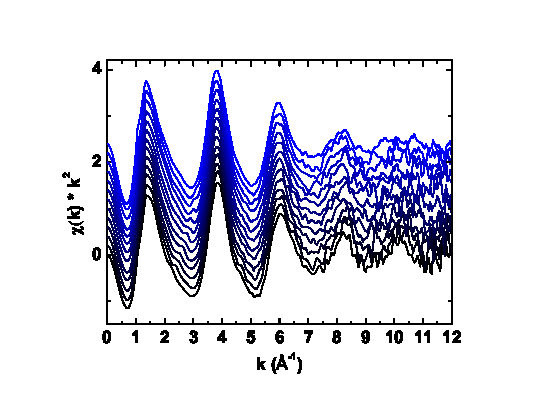
\includegraphics[width=0.5\textwidth]{./chapter_5/exafs_chik.eps}}
	\hspace{-1ex}
	\subfloat[\label{fig:label:exafs_chir}]{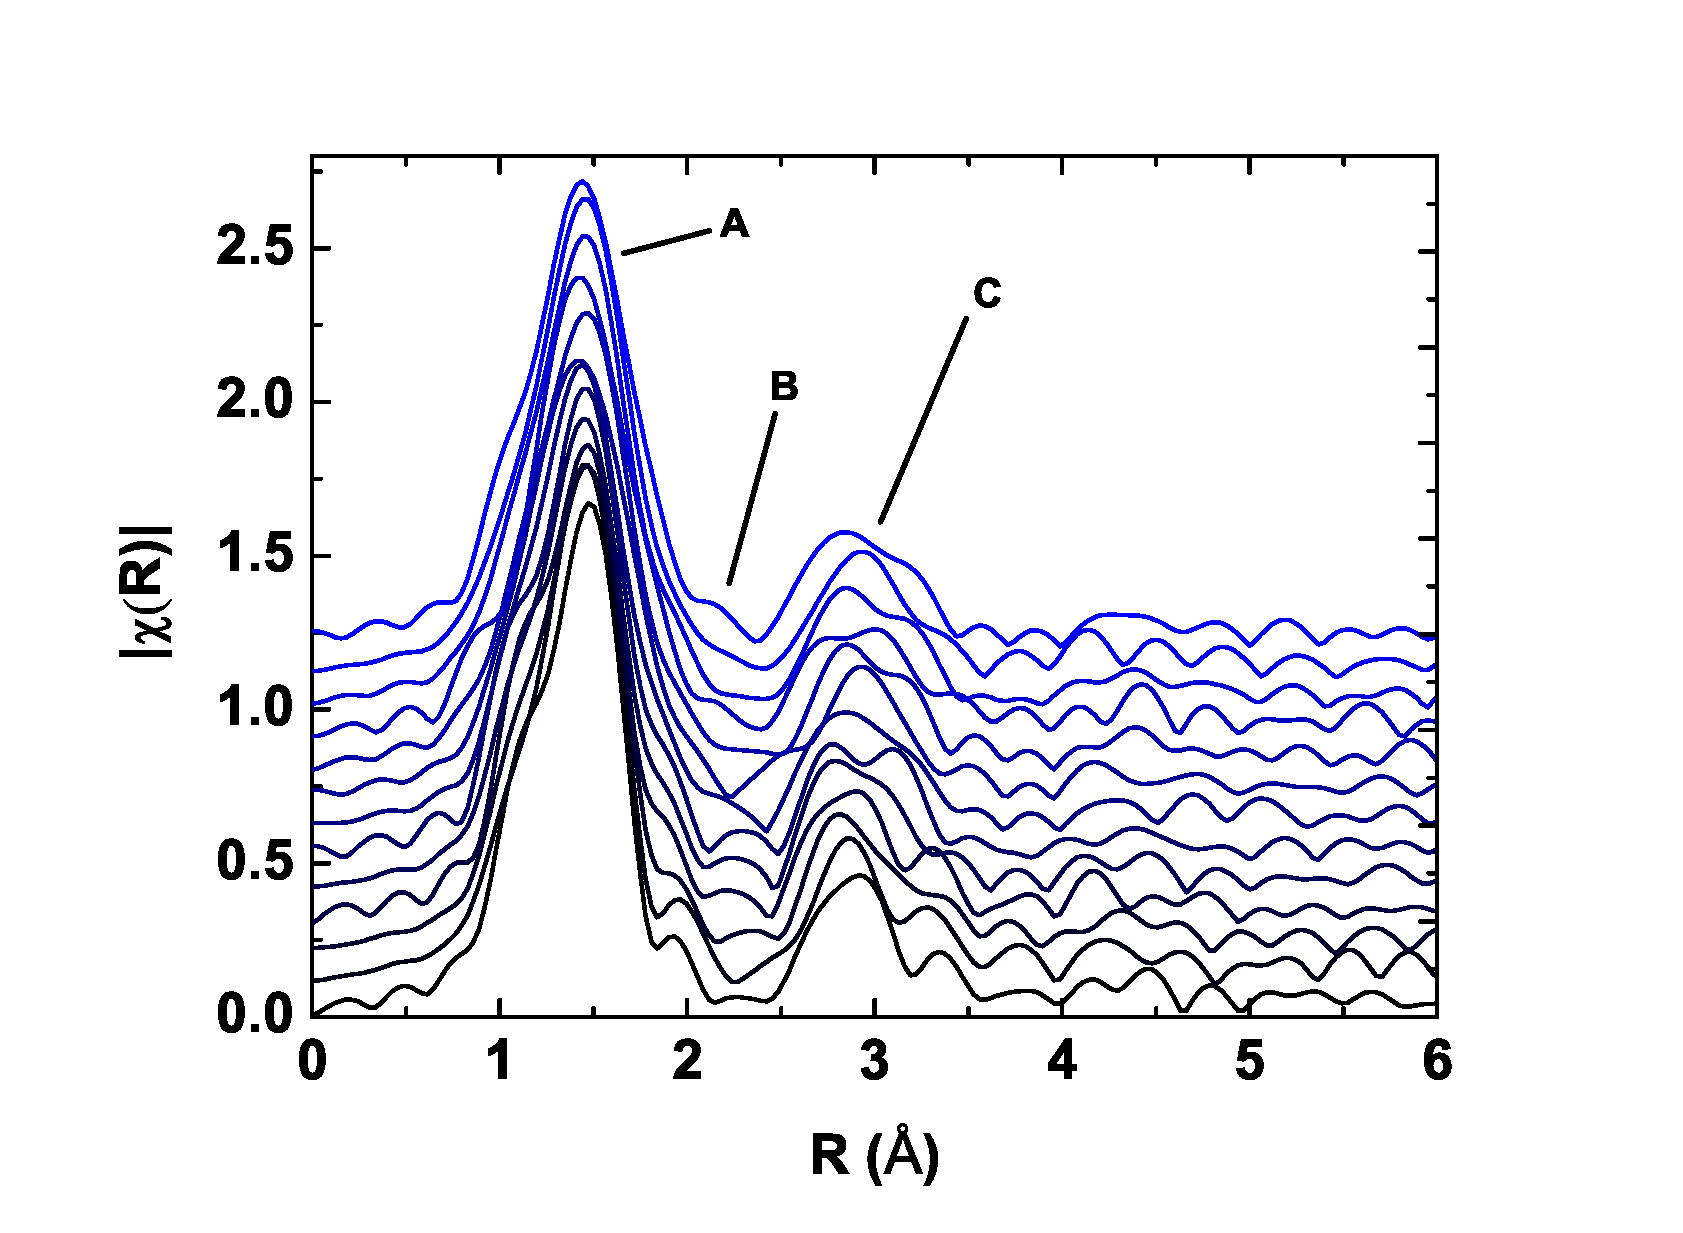
\includegraphics[width=0.5\textwidth]{./chapter_5/exafs_chir.eps}}
	\caption{(a) The XAS absorption spectra of amorphous Ta$_{2}$O$_{5}$ and Ta$_{x}$Ge$_{1-x}$O$_{2+x/2}$ thin films. The spectra are vertically shifted for easier viewing. Film compositions are identical to those investigated in the PDF. The inset shows the variation of the (unshifted) L-III line with composition. (b) $\chi(k)$ and (c) $|\chi(R)|$ spectra as a function of composition. $|\chi(R)|$ is plotted without a phase shift. The top-most spectrum for each figure corresponds to the spectrum of pure Ta$_{2}$O$_{5}$.}
	\label{fig:xas}
\end{figure*}

We take advantage of the chemical specificity of XAS to examine the Ta L-III edge to investigate the fine structure, or EXAFS centered around Ta atoms. The edge (Figure \ref{fig:label:xas_mu}) corresponds to dipole-allowed transitions 2p$_{3/2}\rightarrow$ 5d$_{5/2}$, 5d$_{3/2}$. There is no energy shift in the position of the white-line peak, which indicates that the formal valence of Ta is constant as Ge is incorporated into the amorphous structure. We also observe a monotonic decrease in the height of the L-III edge with Ge incorporation (Figure \ref{fig:label:xas_mu} inset). This suggests that Ge doping results in the increase of 5d occupation \cite{Qi1987}.

The behaviors of $k^{2}\chi(k)$ and its Fourier transform are plotted as a function of Ta cation composition in Figure \ref{fig:label:exafs_chik} and \ref{fig:label:exafs_chir}. Here, $\chi(R)$ is not corrected for the photoelectron phase shift. The sample-to-sample variation of the $k^{2}\chi(k)$ spectra is difficult to interpret, so we limit ourselves to examining qualitative variations in the $\chi(R)$ spectra. We see that the position of the inner shell peak A is roughly independent of composition, whereas peak B changes in peak position and amplitude, though the exact behavior of the latter is hard to discern from the spectra alone. Other prominent features are the outer shell peaks (C), which show high variability in peak shape and position.

To gain a quantitative understanding of the EXAFS data, we fit four experimental EXAFS spectra to amorphous structural models of similar compositions derived from \emph{ab-initio} MD. Note, the calculated dielectric constants of our simulated structures show a similar trend to experimental values \cite{Naoi2018jap}, which indicate that our simulated structures possess local structures that are similar to those of the experimental samples (see Supplementary Material \cite{Supp}). The resulting fit parameters are tabulated in Table \ref{table:exafs2}, and the fitted EXAFS in $k$ and $R$-space are shown in Figure \ref{fig:exafs_fitted}. Our fits to pure Ta$_{2}$O$_{5}$ yield two Ta-O shells at 1.88 and 2.03 \AA \;(Table \ref{table:exafs2}), which shows the existence of two oxygen sites (I and II). These bond distances are close to our experimental results obtained from analysis of the PDF data (Figure \ref{fig:grfq}), although the PDF is able to resolve only a single Ta-O peak.

By fixing the amplitude reduction factor to  $S_{o} = 1.0$, we estimated the coordination numbers in the EXAFS equation. We obtain $N = 2.92$ and $N = 1.20$ for the coordination numbers of the two Ta-O inner shells (Table \ref{table:exafs2}), hence the average coordination number of the Ta-O inner shell is $N_{Ta-O} \sim 4$. This is lower than one might expect based on coordination numbers of crystalline Ta$_{2}$O$_{5}$, which is six or seven \cite{Aleshina2002, Lee2013, Stephenson1971}. It is known however, that the coordination number of metal-oxygen (M-O) complexes in amorphous melts and glasses can be significantly lower than in the corresponding crystalline phase, which holds true especially for cations with low fields and larger ionic radii, \emph{i.e.}, poor network formers \cite{Skinner2014}. For comparison, we calculate the cation field strength of Ta-O and Ge-O as $F = Z_{M}/(r_{MO} - 1.24)^{2}$, where $Z_{M}$ is the formal charge of the cation, $r_{MO}$ is the M-O bond distance, and 1.24 is the ionic radius of Oxygen \cite{Shannon1969}. Using experimentally derived M-O bond distances, we determine $F_{Ta_{2}O_{5}} = 10.5$ $e/\text{\AA}^{2}$ and $F_{GeO_{2}} = 16.7$ $e/\text{\AA}^{2}$. In contrast, $F_{SiO_{2}} = 26$ $e/\text{\AA}^{2}$ \cite{Skinner2014}. Since Ta-O tends to be a poor network former, we expect the coordination numbers to be reduced and indeed our values are very much consistent with values from a recent EXAFS study by Bassiri et al. \cite{Bassiri2015}.

\begin{table}[ht]
\centering
\setlength{\tabcolsep}{5pt}
\begin{tabular}{llcccc}
\hline\hline
Model & Path & $R$(\AA) 
& $\Delta R$(\AA) & $N$ & $\sigma^{2}$ (\AA$^{2}$) \\
\hline
{} & Ta-O  			   	   & 1.88  & { }0.058 & 2.92 & 0.004 \\ 
Ta$_{2}$O$_{5}$	   & Ta-O  & 2.03  & { }0.047 & 1.20 & 0.004 \\ 
(Ta$_{16}$O$_{40}$)& Ta-Ta & 3.10  &   -0.001 & 1.05 & 0.005 \\
{} & Ta-O  			   	   & 3.53  &   -0.240 & 2.60 & 0.007 \\
{} & Ta-Ta 			   	   & 3.74  &   -0.001 & 0.21 & 0.005 \\
\hline
{}								   & Ta-O  & 1.91 &   -0.020 & 3.93 & 0.006 \\ 
Ta$_{0.93}$Ge$_{0.07}$O$_{\delta}$ & Ta-O  & 2.07 & { }0.067 & 0.80 & 0.006 \\
(Ta$_{15}$Ge$_{1}$O$_{40}$)		   & Ta-Ta & 3.10 &   -0.280 & 0.43 & 0.001 \\
{} 								   & Ta-O  & 3.52 &   -0.051 & 2.78 & 0.008 \\
\hline 
{}& Ta-O  									& 1.92 &   -0.051 & 4.13 & 0.006  \\ 
Ta$_{0.75}$Ge$_{0.25}$O$_{\delta}$	& Ta-O  & 2.11 & { }0.041 & 1.69 & 0.006  \\
(Ta$_{12}$Ge$_{4}$O$_{40}$) 		& Ta-Ta & 3.02 &   -0.257 & 6.17 & 0.011  \\
{}& Ta-Ge 									& 3.07 &   -0.084 & 12.7 & 0.020  \\
\hline 
{} & Ta-O   							 	& 1.93 & { }0.071 & 5.48 & 0.008 \\ 
Ta$_{0.51}$Ge$_{0.49}$O$_{\delta}$ & Ta-O   & 2.20 & { }0.093 & 1.79 & 0.008 \\
(Ta$_{8}$Ge$_{8}$O$_{40}$)		   & Ta-Ge  & 3.03 &   -0.008 & 7.99 & 0.018 \\
{} & Ta-Ta  							 	& 3.06 &   -0.060 & 14.2 & 0.023 \\
\hline 
\end{tabular}
\caption{EXAFS fit parameters for Ta$_{2}$O$_{5}$ and Ta$_{x}$Ge$_{1-x}$O$_{2+x/2}$ amorphous thin films on silicon nitride for four different compositions. Experimentally derived compositions are indicated without parenthesis, while the compositions of models generated via simulations are shown within parentheses.}
\label{table:exafs2}
\end{table}

\begin{figure*}[t]
\centering
	\subfloat[\label{fig:label:exafs_ta2o5}]{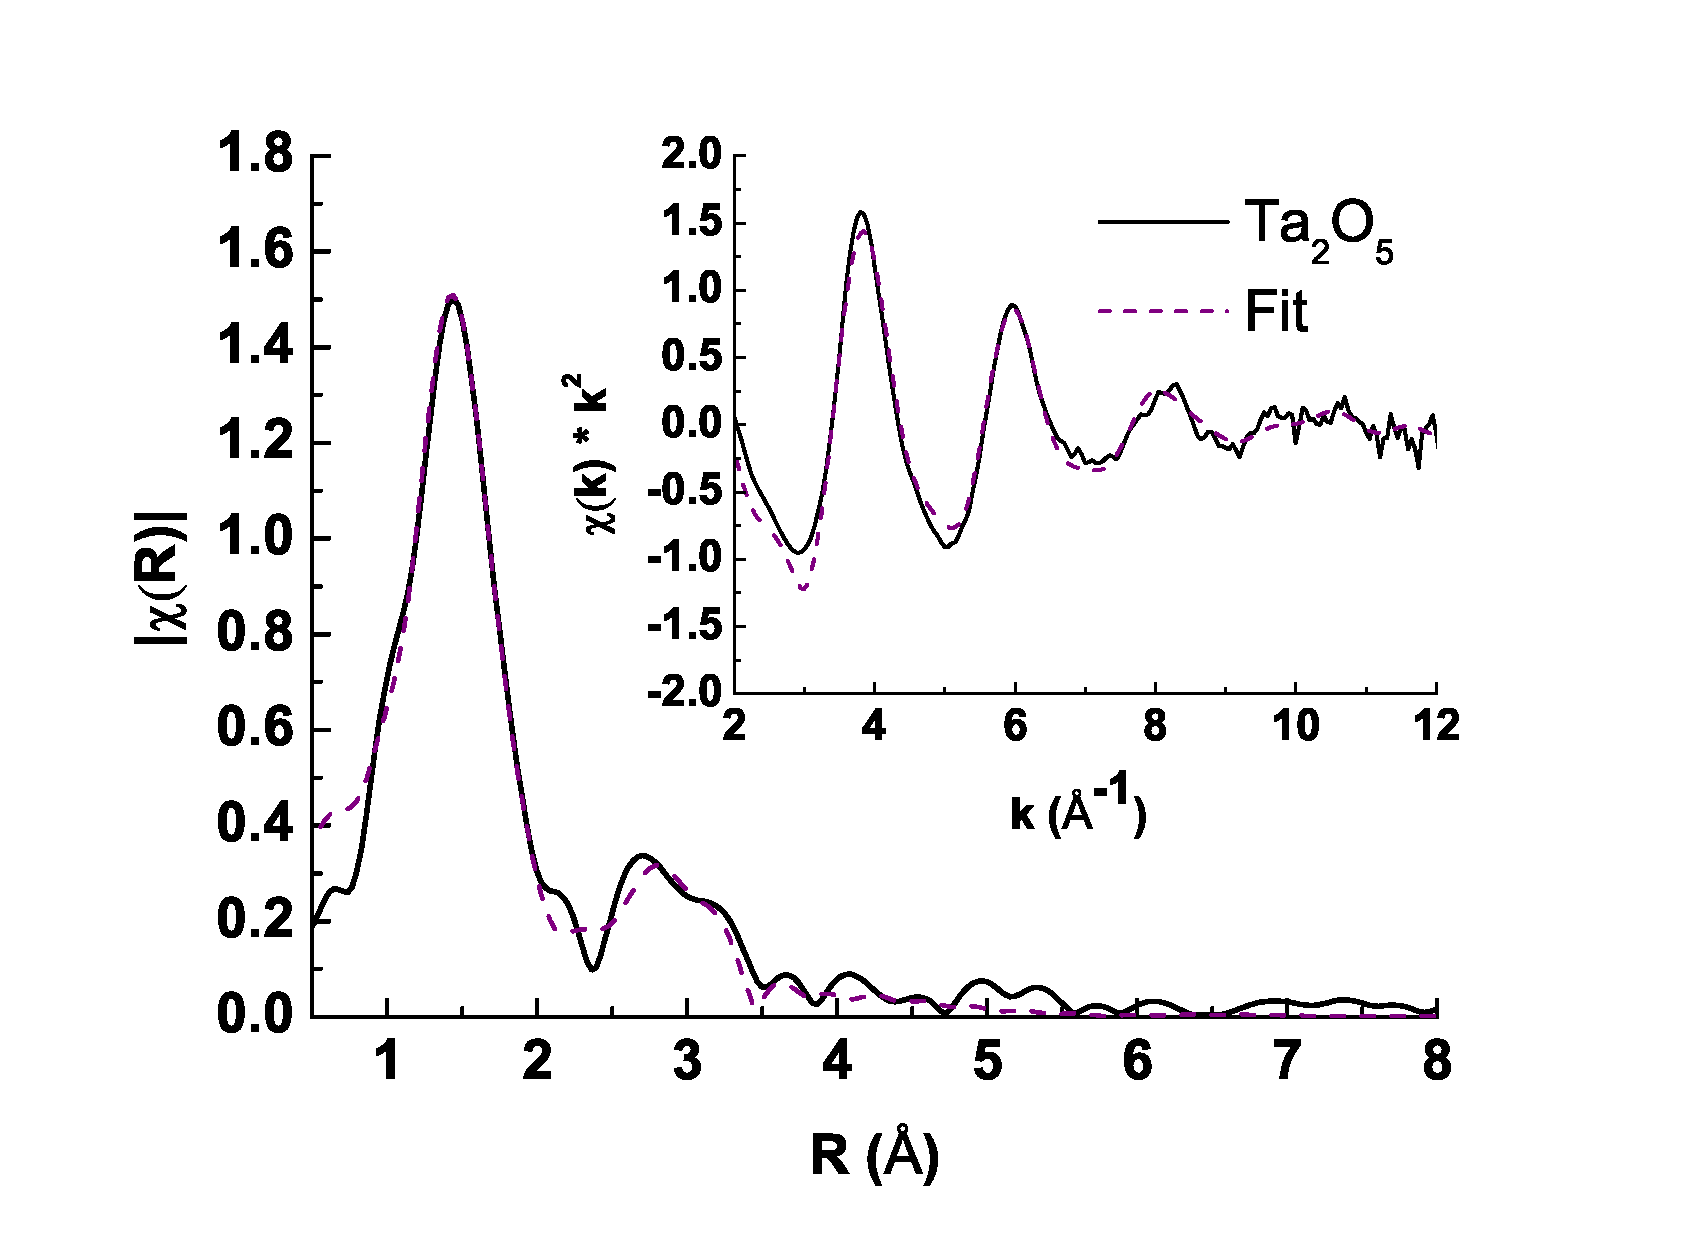
\includegraphics[width=0.5\textwidth]{./chapter_5/exafs_ta2o5.eps}}
	\hspace{-8ex}
	\subfloat[\label{fig:label:exafs_ta15}]{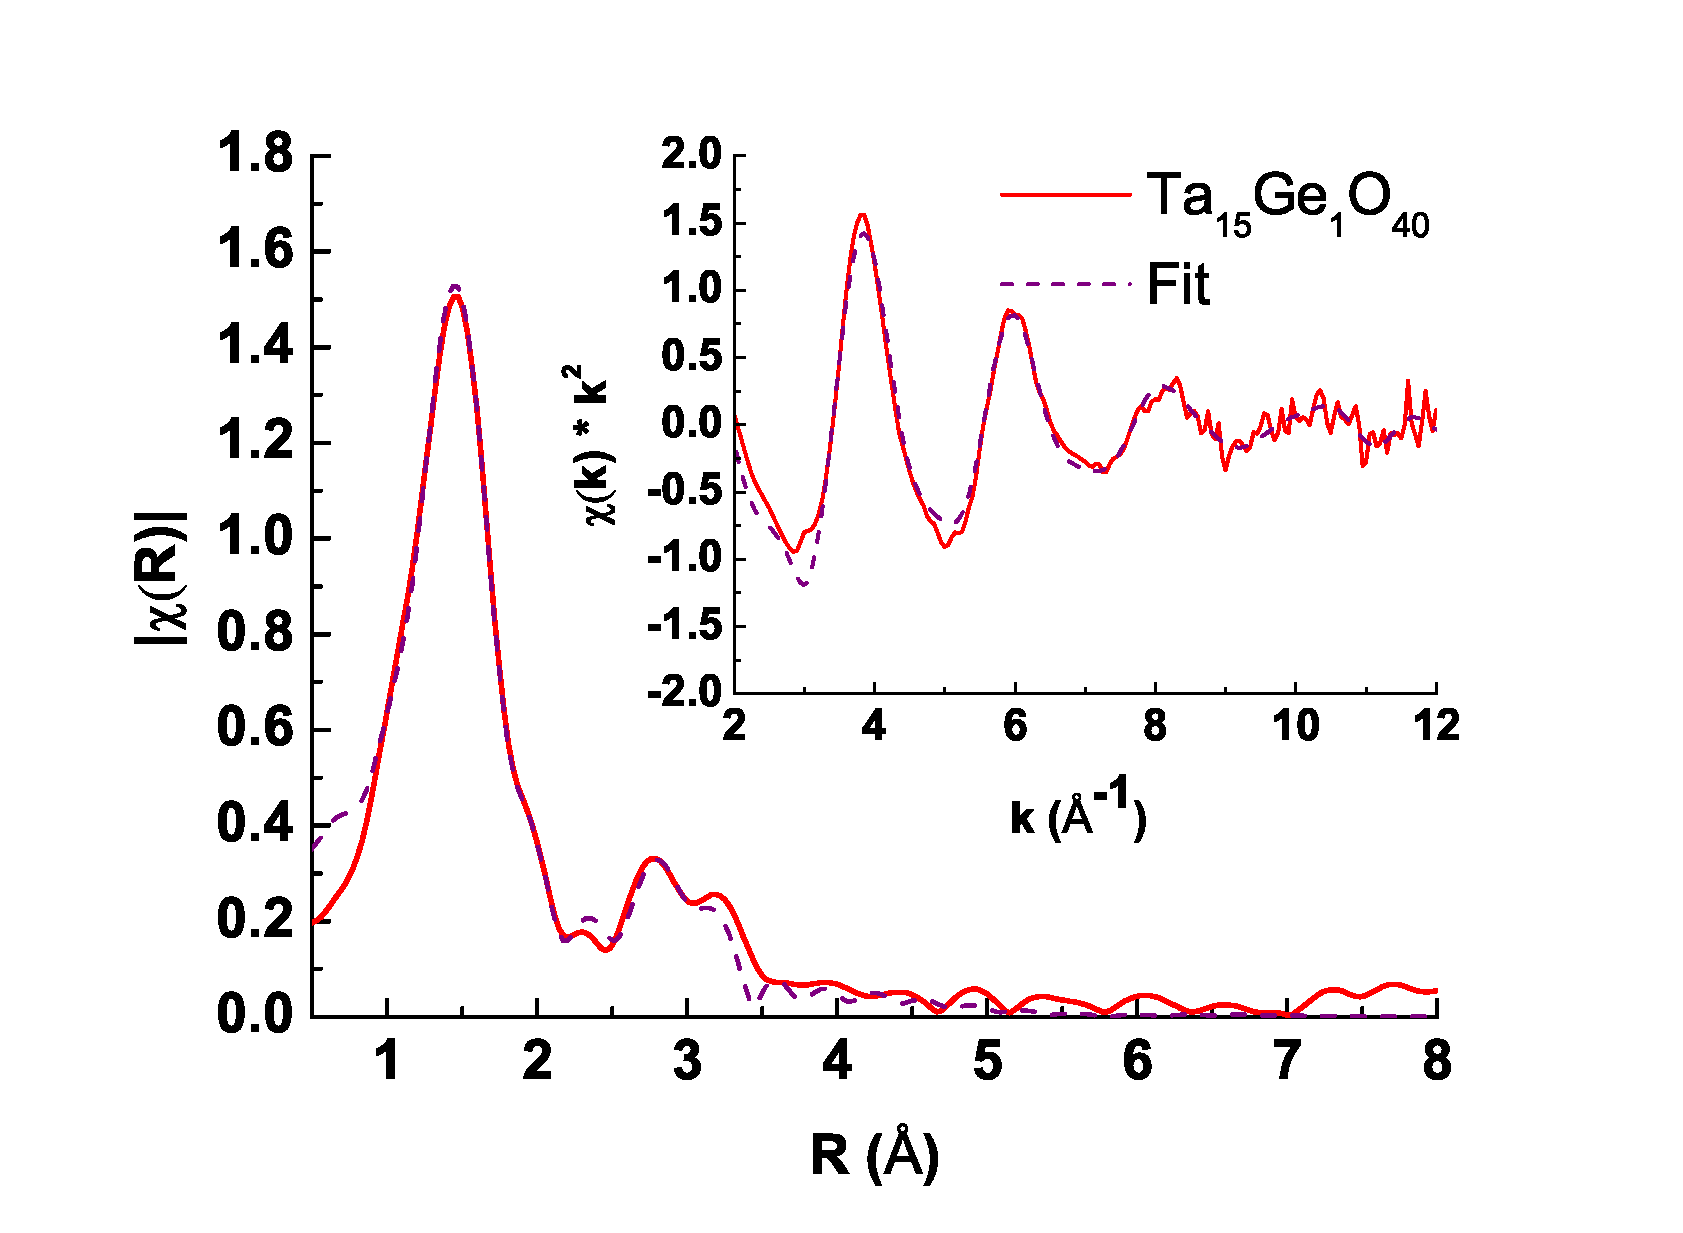
\includegraphics[width=0.5\textwidth]{./chapter_5/exafs_ta15.eps}}
	\qquad
	\subfloat[\label{fig:label:exafs_ta12}]{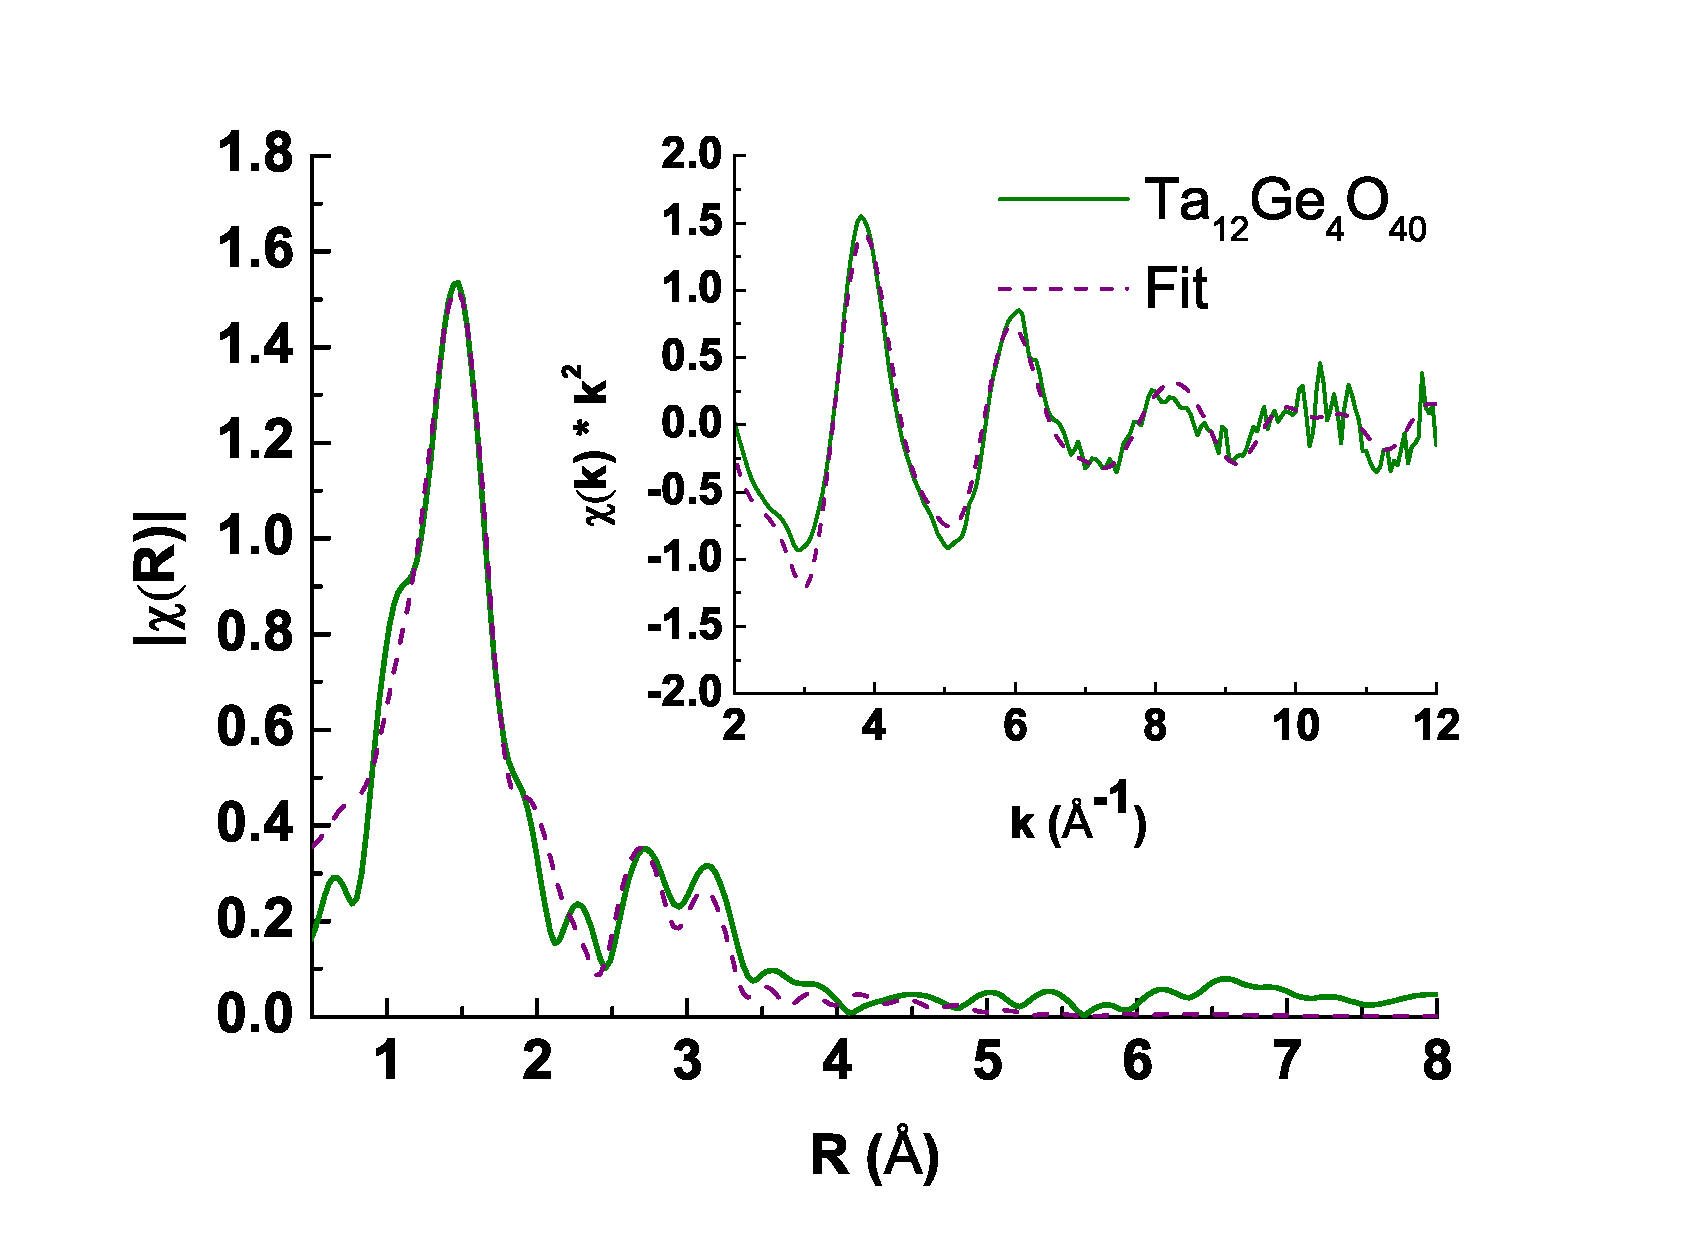
\includegraphics[width=0.5\textwidth]{./chapter_5/exafs_ta12.eps}}
	\hspace{-8ex}
	\subfloat[\label{fig:label:exafs_ta8}]{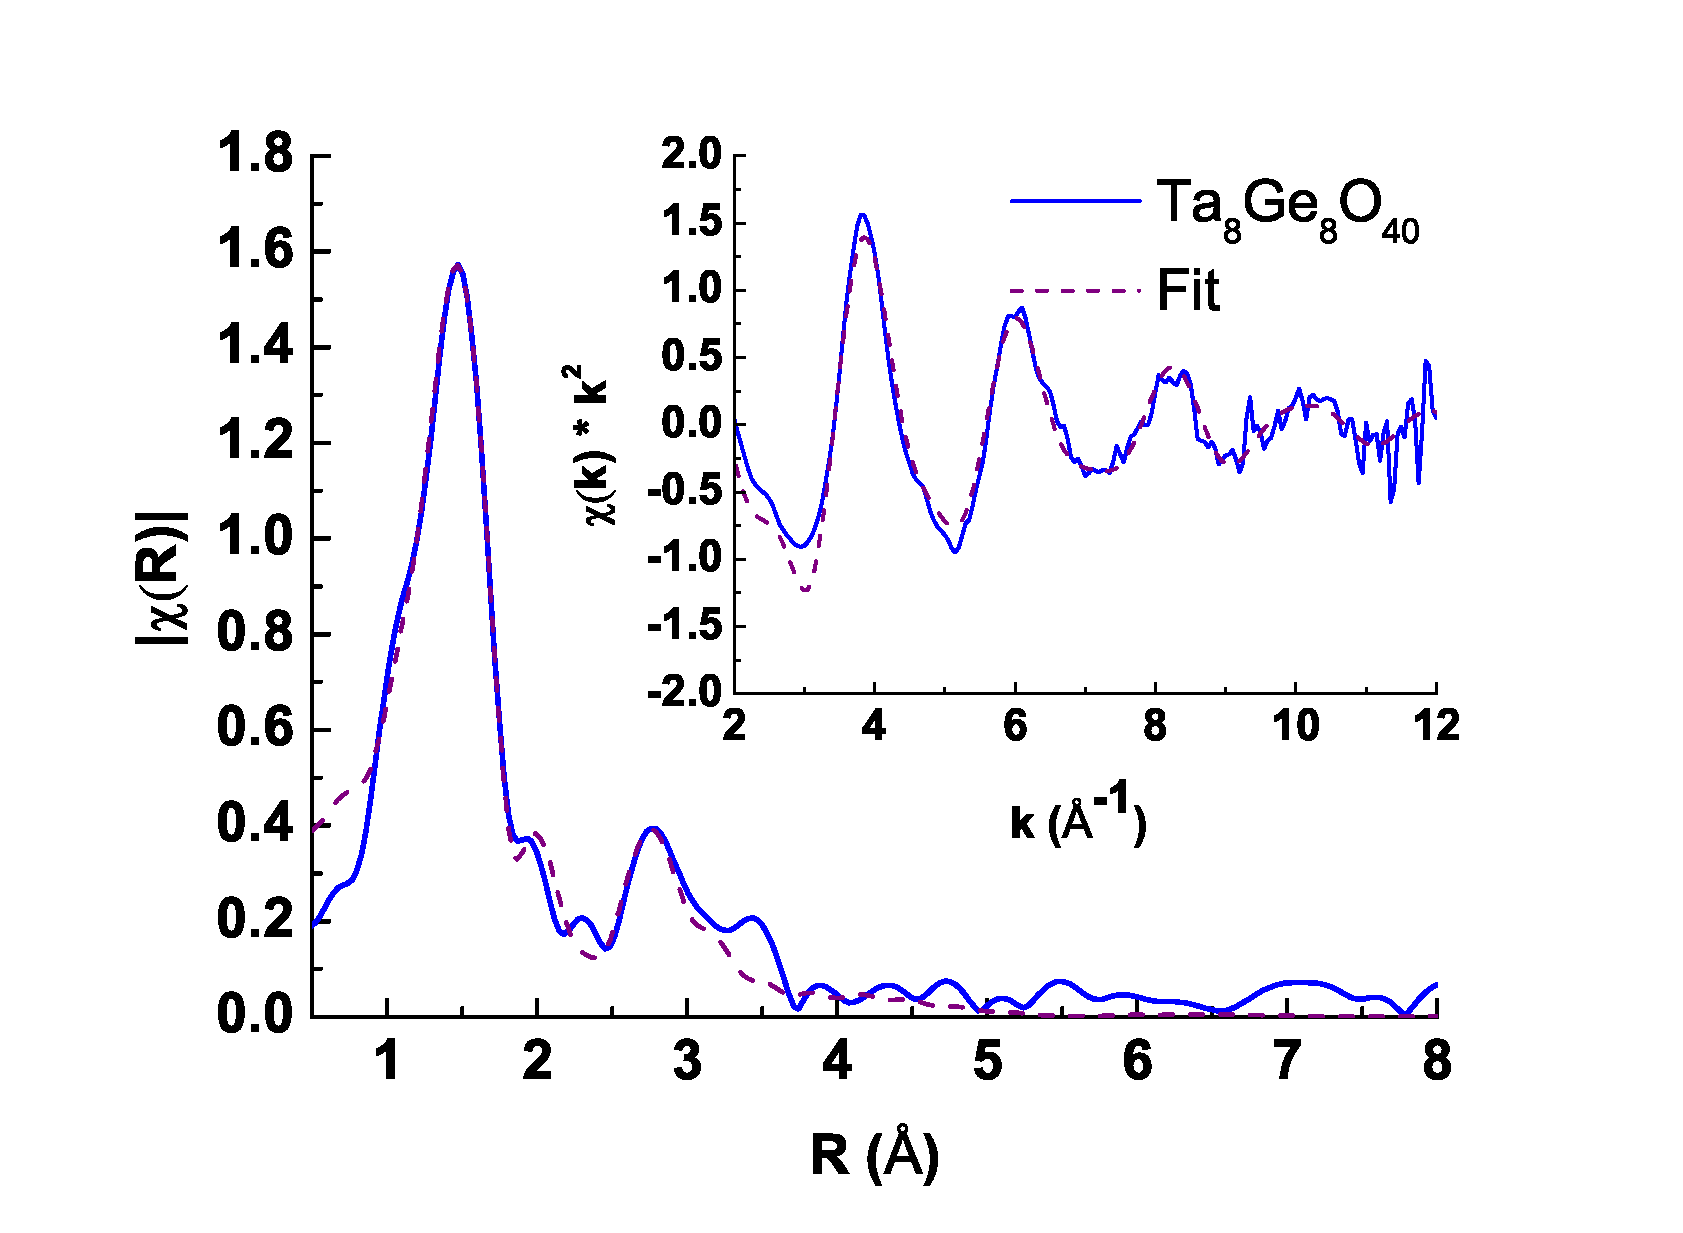
\includegraphics[width=0.5\textwidth]{./chapter_5/exafs_ta8.eps}}
	\caption{Fitted EXAFS $\chi$(k) and $\chi$(R) spectra for (a) pure Ta$_{2}$O$_{5}$, (b) Ta$_{15}$Ge$_{1}$O$_{40}$, (c) Ta$_{12}$Ge$_{4}$O$_{40}$, and (d) Ta$_{8}$Ge$_{8}$O$_{40}$. The dashed lines are the best fit lines for each spectrum.}
	\label{fig:exafs_fitted}
\end{figure*}

The addition of GeO$_{2}$ into Ta$_{2}$O$_{5}$ results in conspicuous changes to pair bond distances. 
We present the Ta(Ge)-O bond distances based on our PDF data, $r_{Ta(Ge)-O}^{PDF}$, in Figure \ref{fig:label:ta-o}.
The Ta-O, Ta-Ta, and Ta-Ge bond distances obtained from our fits to the EXAFS spectra ($r_{Ta-O_{(I,II)}}^{EXAFS}$, $r_{Ta-Ta}^{EXAFS}$, $r_{Ta-Ge}^{EXAFS}$) are shown in Figure \ref{fig:label:ta-ta}. We note that $r_{Ta(Ge)-O}^{PDF}$ is assumed to be composed of overlapping inner shell Ta-O and Ge-O peaks, for which the contribution from the individual peaks depends on the composition. Comparing the PDF data in Figure \ref{fig:label:ta-o} to the EXAFS data in Figure \ref{fig:label:ta-ta} for low levels of GeO$_{2}$, we notice that $r_{Ta-O_{(I,II)}}^{EXAFS}$ is actually increasing with the addition of GeO$_{2}$, most prominently in the second inner shell Ta-O bond distance ($r_{Ta-O_{(II)}}^{EXAFS}$); the first inner shell Ta-O bond distance ($r_{Ta-O_{(I)}}^{EXAFS}$) shows only a modest increase with decreasing $x$. However, the net effect of the change in $r_{Ta-O_{(I,II)}}^{EXAFS}$ results in a less drastic enhancement of $r_{Ta(Ge)-O}^{PDF}$ above linear interpolation of endmember values: at $x = 0.93$ $r_{Ta(Ge)-O}^{PDF}$ is 1.94 \AA. Assuming the contribution of the Ge-O PDF peak to $r_{Ta(Ge)-O}^{PDF}$ is negligible for Ta-rich compositions, the lack of a larger increase in $r_{Ta(Ge)-O}^{PDF}$ implies that the Ta-O structural unit experiences on average, only a modest degree of distortion with low levels of GeO$_{2}$ doping.

\begin{figure*}[t]
\centering
	\subfloat[\label{fig:label:ta-o}]{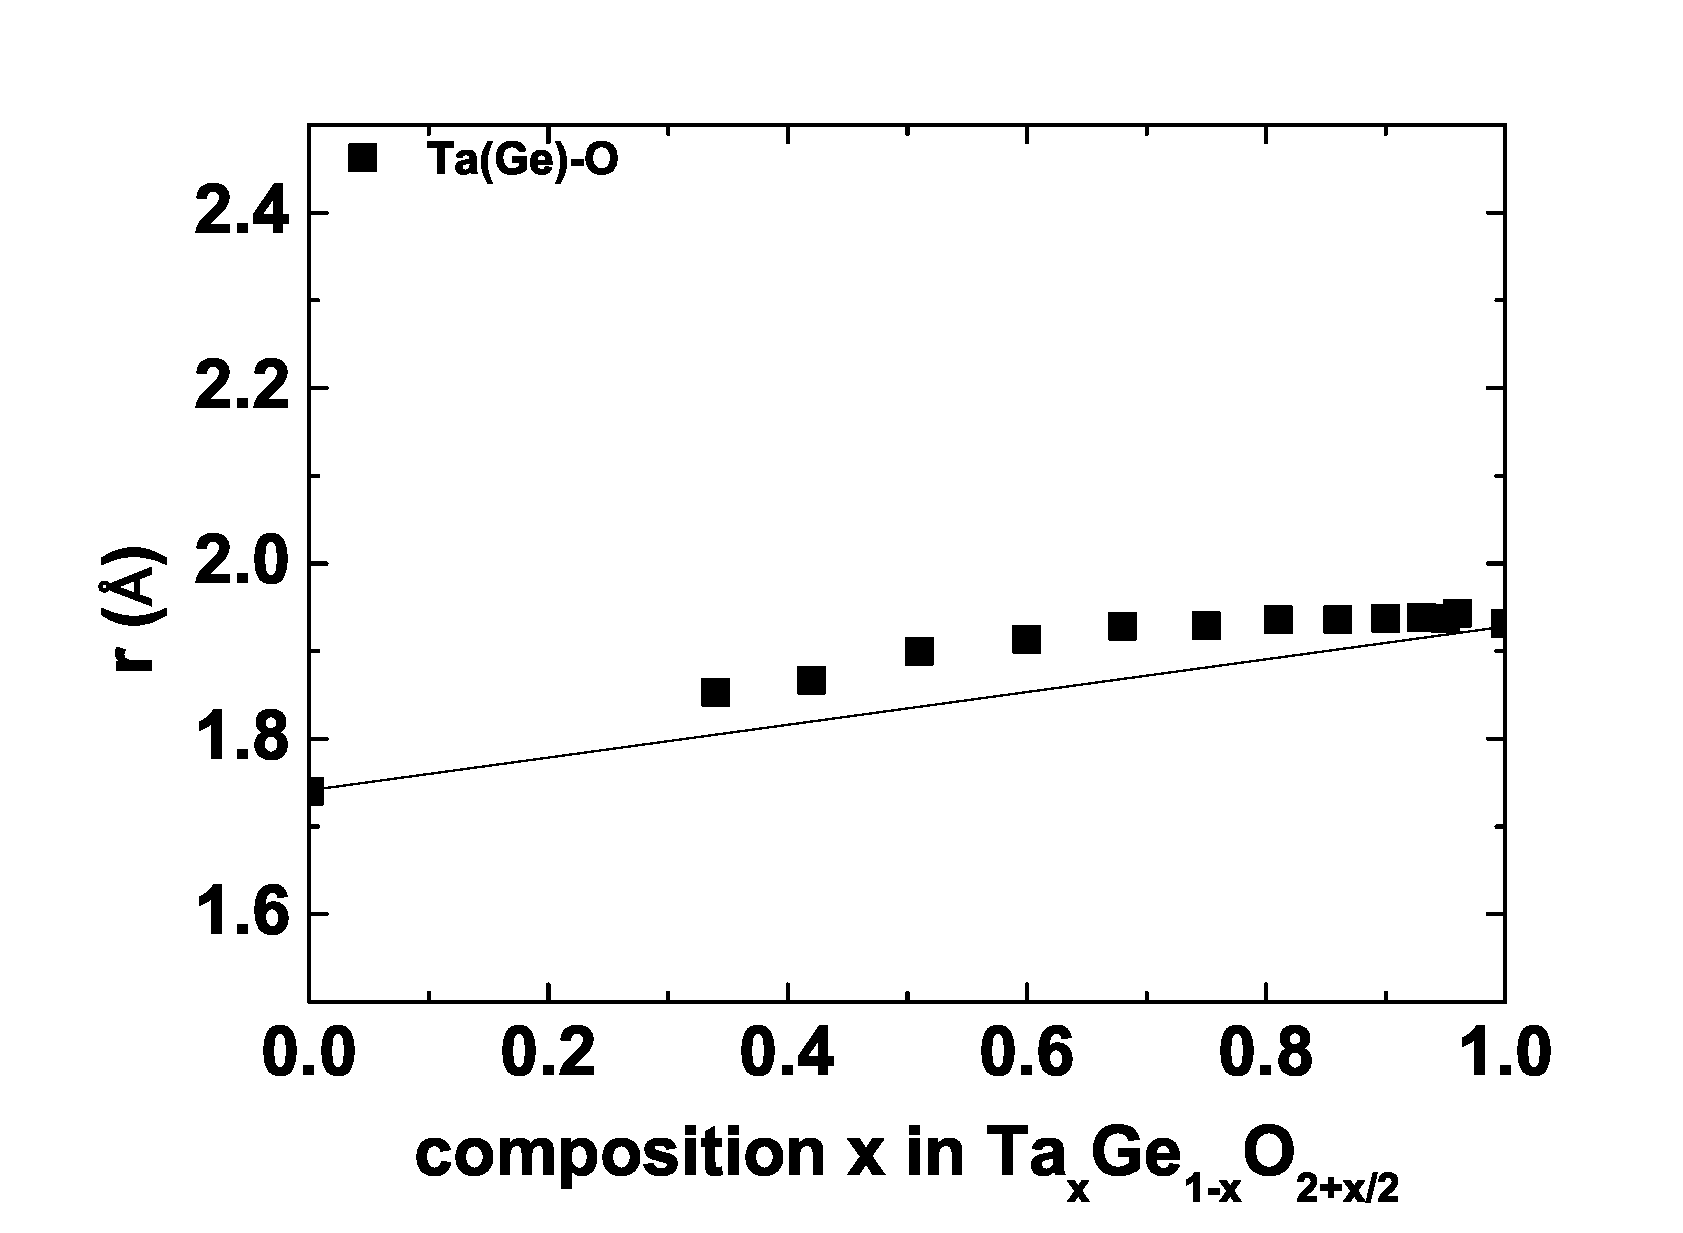
\includegraphics[width=0.5\textwidth]{./chapter_5/ta-o.eps}}
	\hspace{-2ex}
	\subfloat[\label{fig:label:ta-ta}]{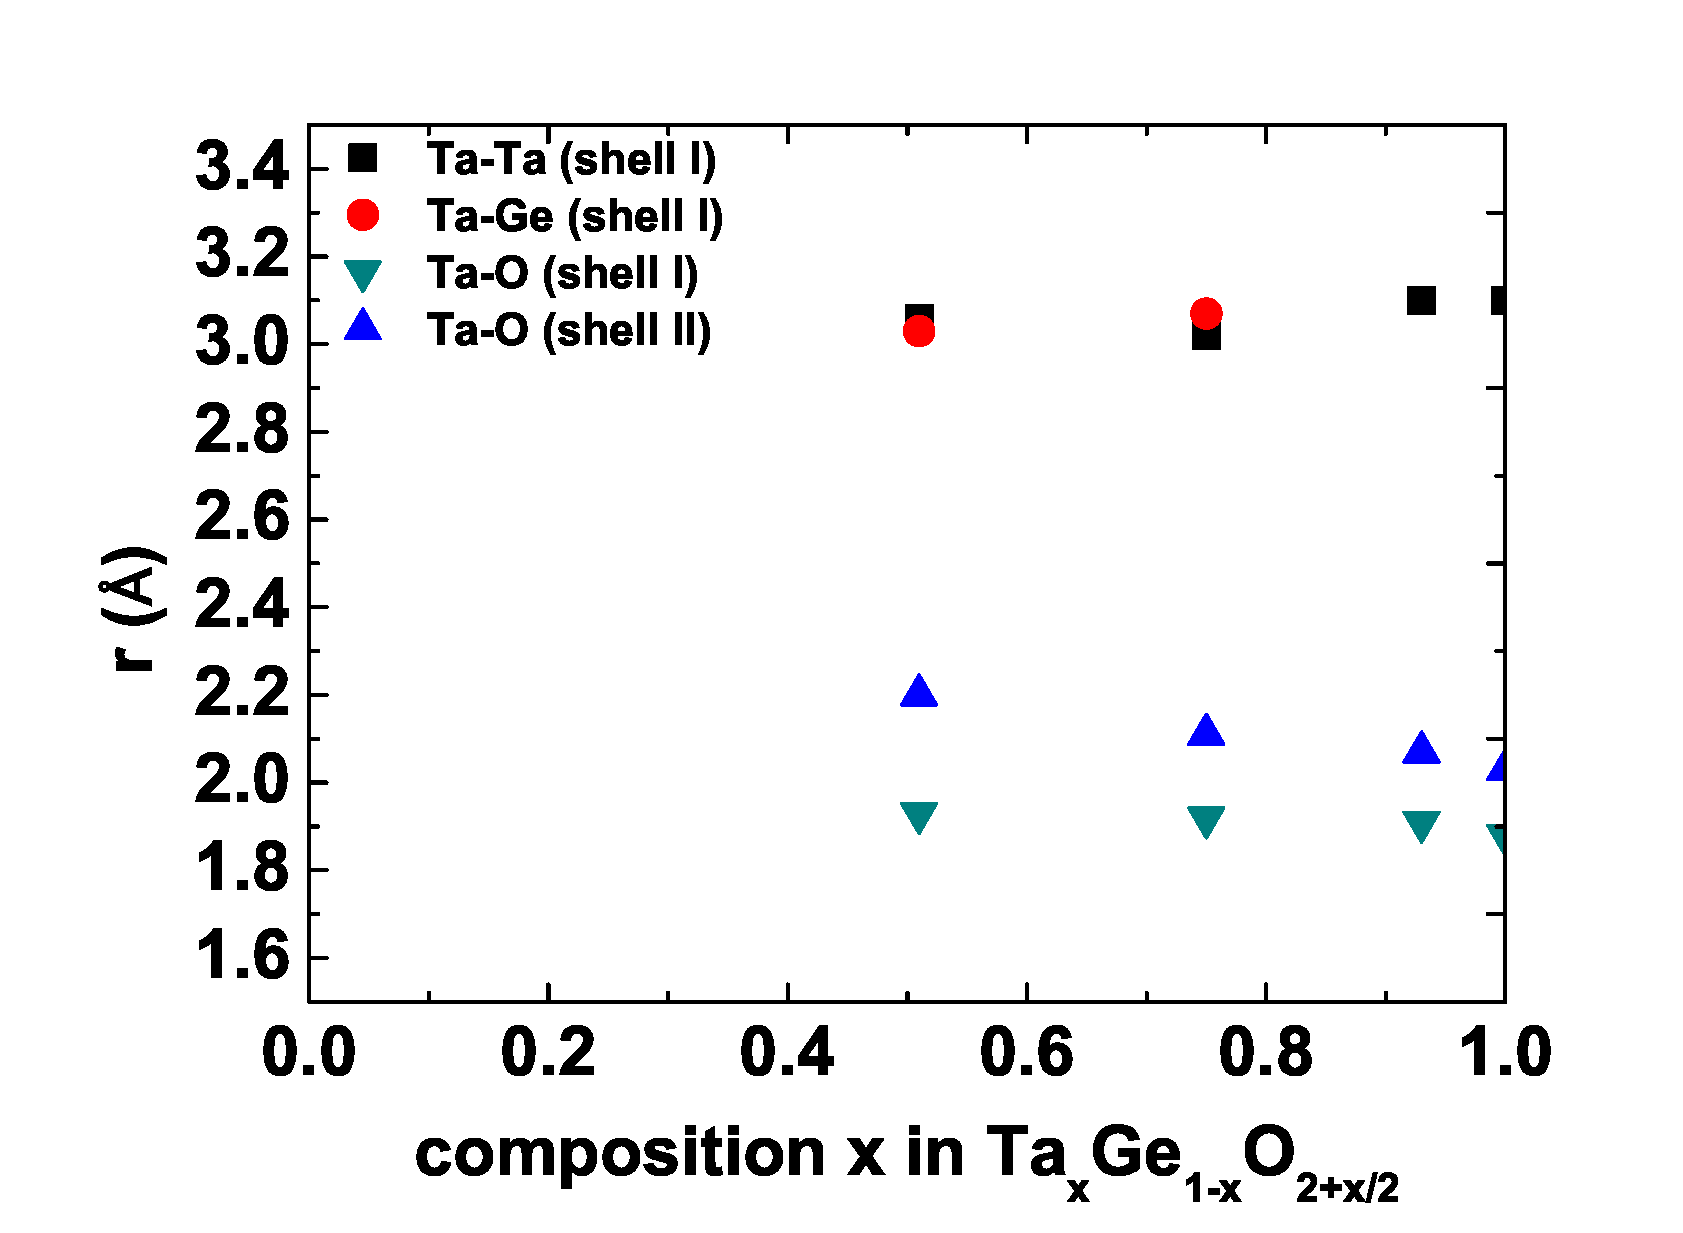
\includegraphics[width=0.5\textwidth]{./chapter_5/ta-ta.eps}}
	\qquad
	\subfloat[\label{fig:label:N}]{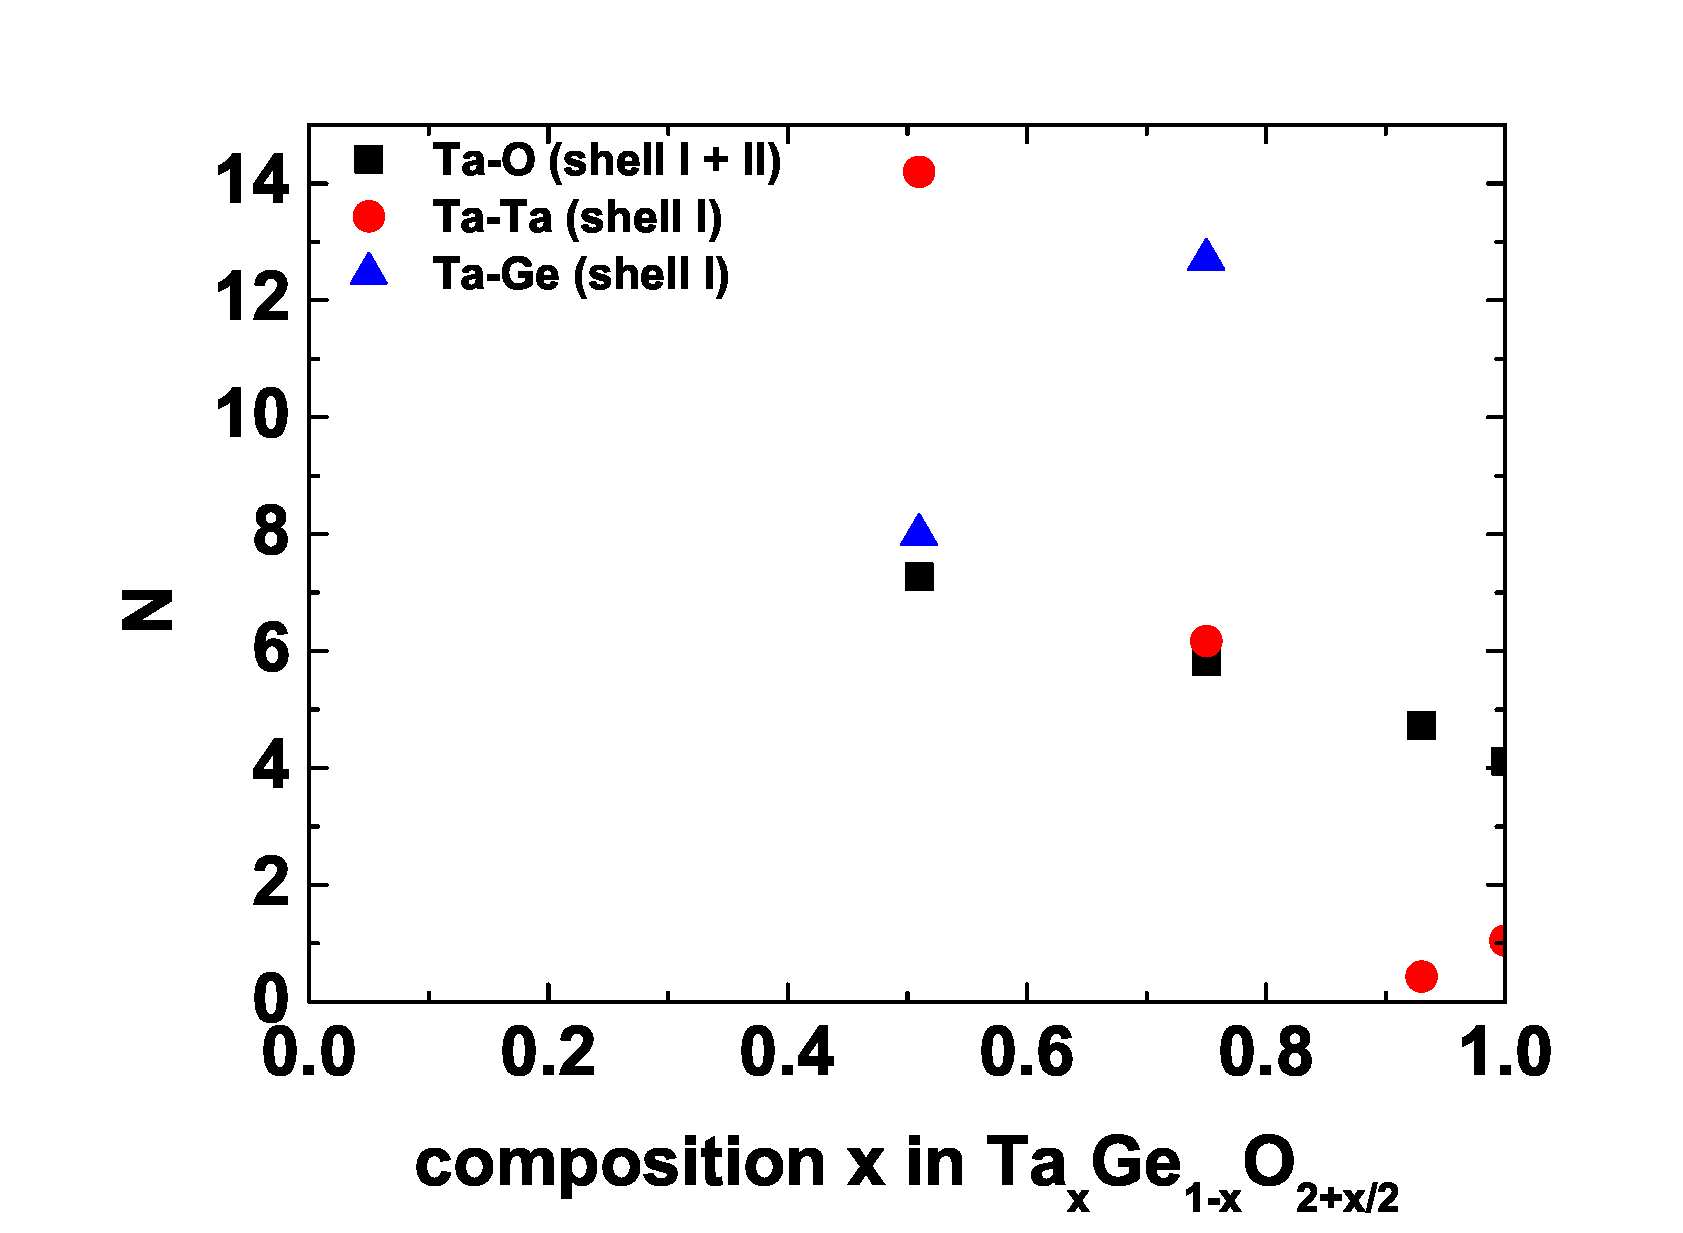
\includegraphics[width=0.5\textwidth]{./chapter_5/N.eps}}
	\hspace{-2ex}
	\subfloat[\label{fig:label:oo_distance}]{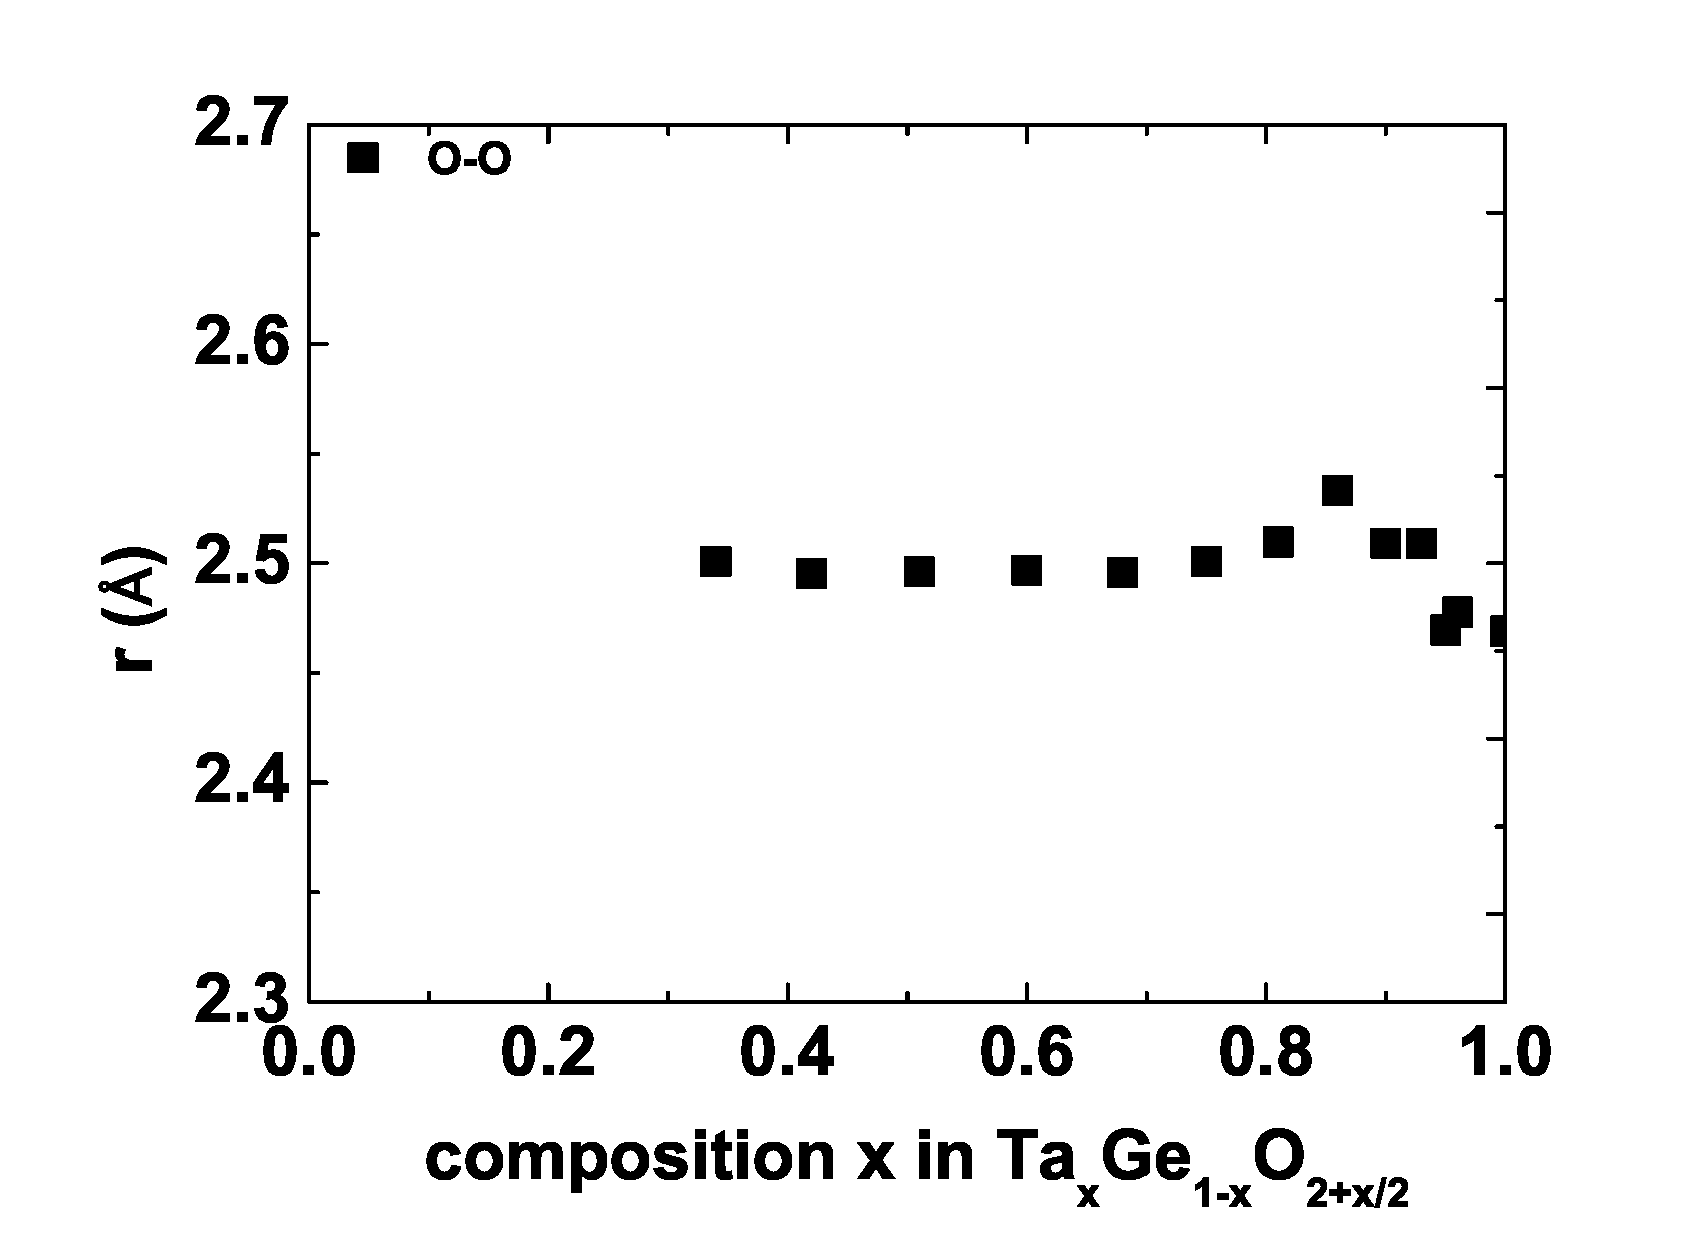
\includegraphics[width=0.5\textwidth]{./chapter_5/oo_distance.eps}}
	\caption{
	(a) Composition dependence of Ta(Ge)-O bond distances determined from PDF data (first peaks in Figure \ref{fig:label:waterfall}). The solid line is an interpolation between values of endmembers.
	(b) Composition-dependent bond distances determined from EXAFS data for Ta-O, Ta-Ta, and Ta-Ge.
	(c) Composition-dependent coordination numbers determined from EXAFS data for Ta-O, Ta-Ta, and Ta-Ge.
	(d) Composition dependence of O-O bond distances determined from PDF data (second peaks in Figure \ref{fig:label:waterfall}). Note, the four compositions in the EXAFS data (b and c) correspond to the four simulated compositions.
	}
	\label{fig:exafs_all}
\end{figure*}  

Further addition of GeO$_{2}$ in Ta$_{2}$O$_{5}$ results in decrease of $r_{Ta(Ge)-O}^{PDF}$---though still above linear interpolation---even as $r_{Ta-O_{(I,II)}}^{EXAFS}$ continues to increase. We presume the decrease in $r_{Ta(Ge)-O}^{PDF}$ with decreasing $x$ is due to increasing contributions from the Ge-O peak to $r_{Ta(Ge)-O}^{PDF}$, though without explicit knowledge of the Ge-O bond distance ($r_{Ge-O}$), a definitive conclusion is not achievable. By contrast, $r_{Ta-Ta}^{EXAFS}$ and $r_{Ta-Ge}^{EXAFS}$ do not demonstrate substantial changes with change in $x$ (Figure \ref{fig:label:ta-ta}). The Ta-Ta pair bond distance contracts slightly with decreasing $x$, though the sparseness of the data precludes a definitive trend.

GeO$_{2}$ substitution also elicits a dramatic change in the coordination environment around Ta (Figure \ref{fig:label:N}). Interestingly, as more GeO$_{2}$ is substituted, we see an increase in the Ta-O coordination number. When the composition of Ta and Ge cations are roughly equal, the average inner shell Ta-O coordination increases to roughly $N_{Ta-O} \sim 7$. Ge occupation of Ta$_{2}$O$_{5}$ interstitial sites may lead to increased network connectivity and in turn, increase Ta-O coordination. The most dramatic coordination shift however, occurs for the metal-metal (M-M) pairs, namely Ta-Ta and Ta-Ge. We observe a large coordination increase in the Ta-Ta coordination ($N_{Ta-Ta}$) from $x = 0.93$ to $x = 0.75$, where $N_{Ta-Ta}$ jumps from 0.43 to 6.17. The EXAFS fit at $x = 0.75$ also includes a Ta-Ge shell with a large coordination number of $N_{Ta-Ge} = 12.7$.

We can use our findings from this study to elucidate trends from previous studies on amorphous Ta$_{x}$Ge$_{1-x}$O$_{2+x/2}$ thin films \cite{Naoi2018jap}. Specifically, we wish to address the 1) large decrease in density away from linear interpolation of endmembers in the 0.6 $<$ $x$ $<$ 0.9 Ta cation range and 2) the dielectric enhancement observed in the 0.75 $<$ $x$ $<$ 0.95 range. 

First, we attribute the reduction of density in the specified range to increases in bond distances. Bond distances relate inversely with density: an increase in bond distances will typically result in decreased density. 
Our data is consistent with this expectation: the enhancement of $r_{Ta(Ge)-O}^{PDF}$ above linear interpolation should result in a proportional decrease in density for a given $x$. Also note the overall increase in $r_{O-O}$ with decreasing $x$. This suggests a distortion in the metal-oxygen-metal (M-O-M) structural unit, which may further contribute to local bond distance expansion.

Second, we suggest that changes in the local coordination environment around Ta with GeO$_{2}$ substitution play a role in dielectric enhancement. Prominent features supporting this claim are the sizable shifts in Ta-Ge and Ta-Ta coordination (Figure \ref{fig:label:N}), accompanied by changes in O-O pair bond distances (Figure \ref{fig:label:oo_distance}). Though the data for Ta-Ge coordination is sparse, the jump in Ta-Ge coordination clearly coincides with the transition from the unenhanced to enhanced region, at roughly $x \sim 0.7$ \cite{Naoi2018jap}. The corresponding drop in $N_{Ta\_Ta}$ from $x = 0.5$ to $x = 0.75$ is likely due to reorganization of the local environment such that there is a high Ge occupancy around Ta instead of Ta. The further drop of $N_{Ta\_Ta}$ suggests that the reorganization occurs throughout the enhanced region ($x = 0.75$ and $x = 0.93$). The O-O bond distances obtained from PDF data also provide some evidence of reorganization between $x = 0.75$ and $x = 0.93$ where coordination data from EXAFS is lacking. We observe a significant increase in $r_{O-O}$ from roughly $x = 0.75$ to $x = 0.85$, with a peak at roughly $x \sim 0.85$; further increase in $x$ above $x = 0.85$ results in the decrease of the O-O bond distance (Figure \ref{fig:label:oo_distance}). We surmise that local atomic reorganization occurring between 0.5 $<$ $x$ $<$ 0.93 creates local deviations in stoichiometry (for instance, Ge interstitials), enhancing low-frequency polarizabilities and in turn enhancing the dielectric constants. A careful probe of the local environment around Ge, whether determined using EXAFS, PDF, or some other technique, along with measurements of IR spectra in the enhanced region should yield a more complete understanding of the relationship between the low-frequency phonon modes and the local atomic structure. 

\section{Conclusion}
We have investigated the local structure of amorphous Ta$_{2}$O$_{5}$ and Ta$_{x}$Ge$_{1-x}$O$_{2+x/2}$ thin films using PDF, EXAFS, and \emph{ab-initio} MD. The films were sputtered on silicon nitride films to facilitate the background subtraction process, yielding data of very high quality. Reliable distribution functions for both Ta$_{2}$O$_{5}$ and Ta$_{x}$Ge$_{1-x}$O$_{2+x/2}$ could be inferred from the diffraction patterns. The results of PDF analysis were combined with EXAFS to interpret the local structure evolution of Ta$_{x}$Ge$_{1-x}$O$_{2+x/2}$ with changes in composition. The coordination numbers and bond distances of amorphous Ta$_{2}$O$_{5}$ are consistent with values reported in previous studies, while addition of GeO$_{2}$ in Ta$_{2}$O$_{5}$ clearly resulted in substantial alterations to the local environment of pure Ta$_{2}$O$_{5}$. We deduce that bond distance enhancement is directly responsible for suppressions of density observed previously. Finally, we explain the previously observed enhancement in the dielectric constant as a direct consequence of changes in local coordination, which we presume enhances low-frequency vibrational modes. Direct observation of the putative low-frequency modes would confirm our hypothesis.

\section{Acknowledgments}
This work was supported by the U.S. Department of Energy under Grant No. DE-FG02-06ER06-15. This work was performed in part at the Cornell NanoScale Facility, a member of the National Nanotechnology Infrastructure Network, which is supported by the National Science Foundation under Grant No. ECS-15420819. This work is based upon research conducted at the Cornell High Energy Synchrotron Source (CHESS) which is supported by the National Science Foundation and the National Institutes of Health/National Institute of General Medical Sciences under NSF award DMR-1332208. This work made use of the Cornell Center for Materials Research Shared Facilities which are supported through the NSF MRSEC program (DMR-1719875). L.W.T. was partially supported by the Semiconductor Research Corporation Education Alliance with support from the Intel Foundation.

\section{Supplemental Information: Atomic structure determination of mixed amorphous Ta$_{2}$O$_{5}$-GeO$_{2}$ thin films deposited on silicon nitride membranes}

\subsection{Calculation of dielectric constants for T\lowercase{a}$_{x}$G\lowercase{e}$_{1-x}$O$_{2+x/2}$}

\begin{figure}[htp]
\centering
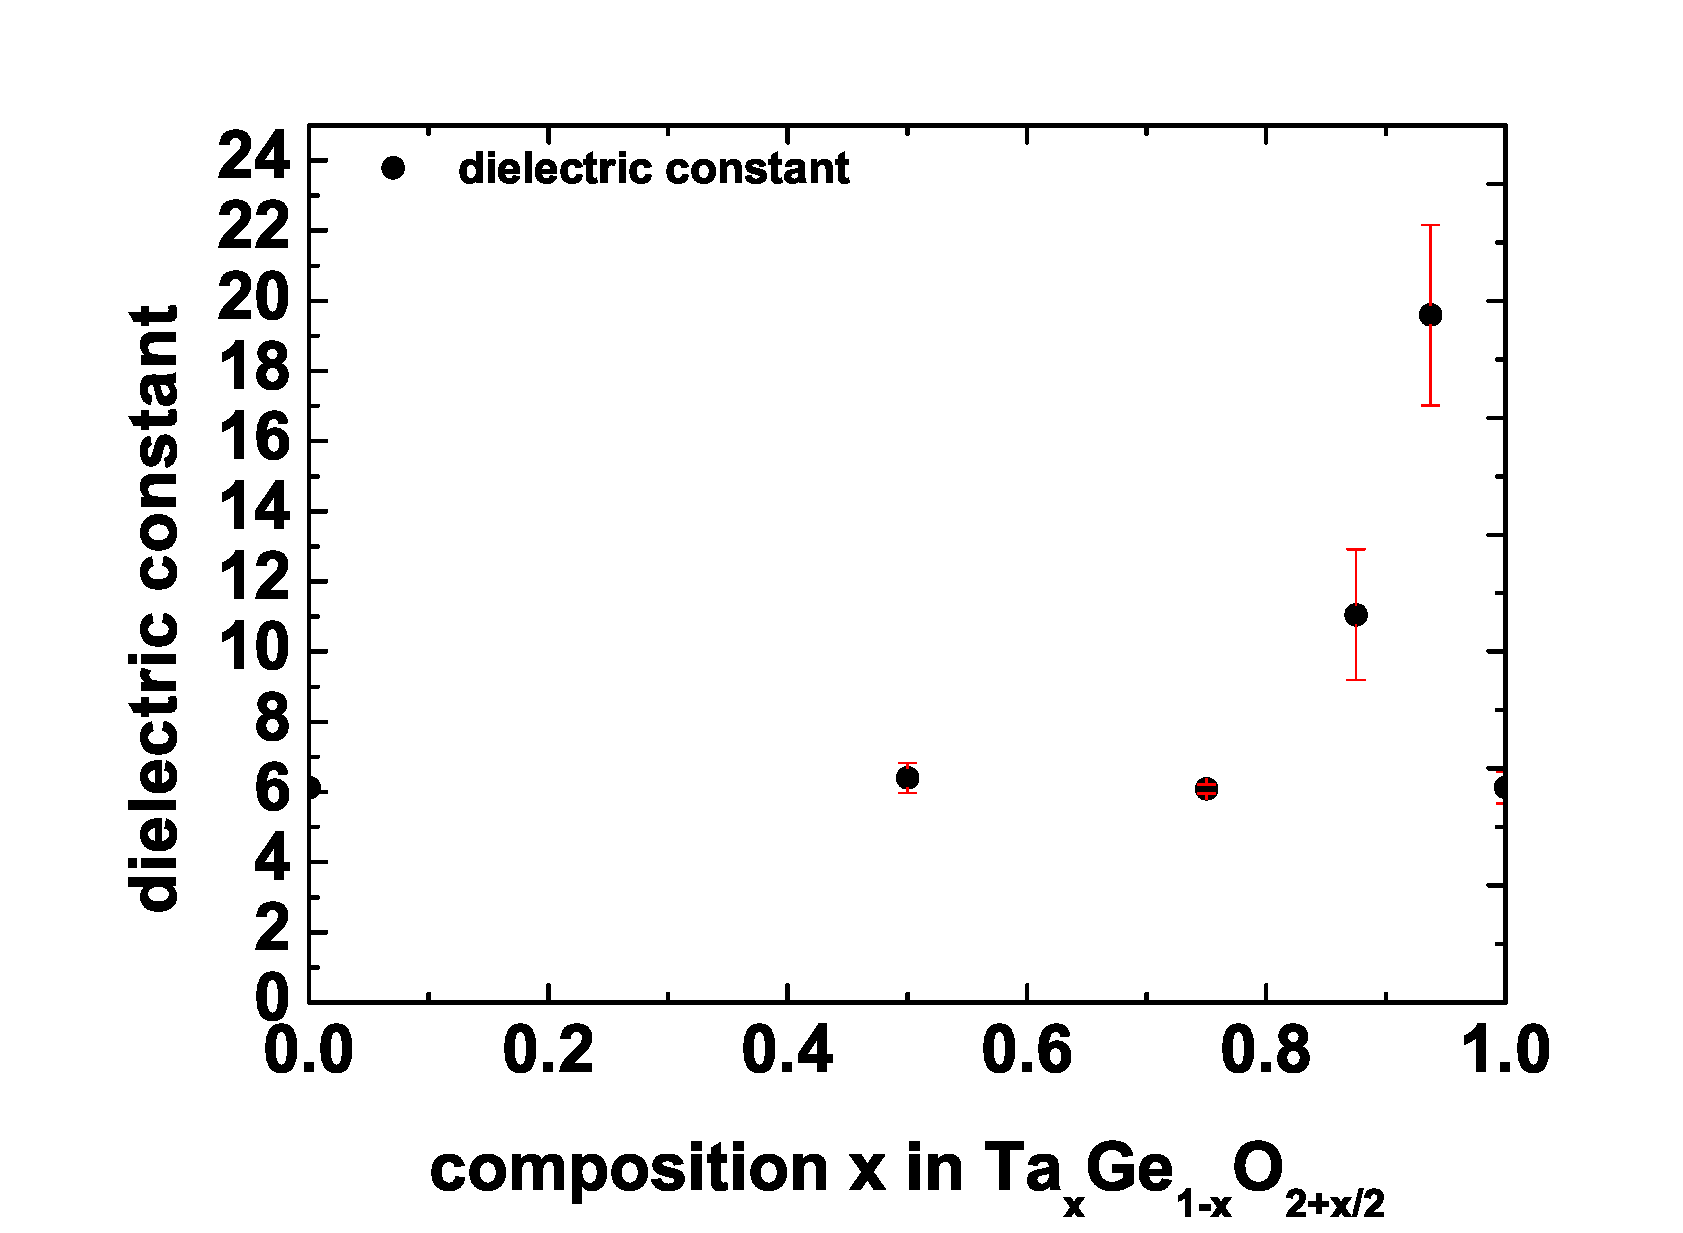
\includegraphics[width=0.7\textwidth]{./chapter_5/dc.eps}
\caption{The calculated dielectric constants for Ta$_{x}$Ge$_{1-x}$O$_{2+x/2}$ as a function of Ta cation composition.}
\label{fig:epsilon}
\end{figure} 

We use density functional perturbation theory (DFPT) \cite{PhysRevLett.58.1861} to calculate the static dielectric tensors for three amorphous structures at each of the following compositions: Ta$_{0.5}$Ge$_{0.5}$O$_{y}$ (Ta$_{8}$Ge$_{8}$O$_{40}$), Ta$_{0.75}$Ge$_{0.25}$O$_{y}$ (Ta$_{12}$Ge$_{4}$O$_{40}$), Ta$_{0.875}$Ge$_{0.1250}$O$_{y}$ (Ta$_{14}$Ge$_{2}$O$_{40}$), Ta$_{0.9375}$Ge$_{0.06250}$O$_{y}$ (Ta$_{15}$Ge$_{1}$O$_{40}$), and pure Ta$_{2}$O$_{5}$. The methods to generate the amorphous structures are described in the main text. Density-functional theory (DFT) calculations were carried out with the Vienna Ab-initio Software Package (VASP) \cite{PhysRevB.47.558,PhysRevB.49.14251,KRESSE199615,PhysRevB.54.11169} using the PBE exchange-correlation functional \cite{PhysRevLett.77.3865}, and the projector augmented wave method \cite{PhysRevB.50.17953,PhysRevB.59.1758}. The Brillouin zone integration was performed using a 3x3x2 Gamma centered k-point mesh \cite{PhysRevB.13.5188}. The kinetic energy cutoff for the plane wave basis was set to 400 eV, and the corresponding cutoff energy for the augmentation function was set to 650 eV.

The dielectric constants are obtained as one third of the trace of the dielectric tensors. The mean dielectric constants, averaged over all three structures at a given composition, are plotted in Figure \ref{fig:epsilon}. The error bars denote the standard deviation of the mean. Although DFT, using semi-local exchange-correlation functionals, accurately predicts structural properties, it is known to underestimate electronic band gaps and is generally less accurate for other electronic properties too. The predicted dielectric constants by DFT underestimate the experimental values. However, we observe the same trend in the dielectric behavior as measured in our previous work \cite{Naoi2018jap}. For structures with $x = 0.5$ and $x = 0.75$, the mean dielectric constant values are close to that of pure amorphous Ta$_{2}$O$_{5}$. However, for more Ta-rich compositions ($x = 0.875$ and $x = 0.9375$), the values show a dramatic increase like the one observed experimentally. This agreement indicates that our simulated structures possess local structures similar to those of the experimental samples, justifying our choice of using them to fit the EXAFS spectra.




% chapter 6
\chapter{Relation Between Dielectric Properties and Structure in Complex Amorphous and Crystalline Thin Film Oxides}

This chapter is adapted from T. A. Naoi and R. B. van Dover: ``Relation Between Dielectric Properties and Structure in Complex Amorphous and Crystalline Thin Film Oxides'' in preparation.

% ABSTRACT
\section{Abstract}
We have used off-axis magnetron sputtering to explore changes in the structural and dielectric properties of pseudo-ternary thin film dielectrics as a function of composition. We investigated four different oxide systems: (HfO$_{2}$)$_{1-x}$(SiO$_{2}$)$_{x}$, (HfO$_{2}$)$_{1-x}$(GeO$_{2}$)$_{x}$, (Nb$_{2}$O$_{5}$)$_{1-x}$(GeO$_{2}$)$_{x}$, and (Ta$_{2}$O$_{5}$)$_{1-x}$(SnO$_{2}$)$_{x}$. The diffraction patterns of (HfO$_{2}$)$_{1-x}$(SiO$_{2}$)$_{x}$ and (HfO$_{2}$)$_{1-x}$(GeO$_{2}$)$_{x}$ were highly similar, where the onset of crystallinity was slightly higher for HfO$_{2}$ films doped with SiO$_{2}$. However, the similarity in diffraction pattern does not translate into comparable dielectric behavior. We obtain a maximum dielectric constant of $\varepsilon_{r} = 28$ at 96 at$\%$ Hf for (HfO$_{2}$)$_{1-x}$(SiO$_{2}$)$_{x}$ whereas for (HfO$_{2}$)$_{1-x}$(GeO$_{2}$)$_{x}$ $\varepsilon_{r}$ is only 19. The refractive indices vary linearly with composition for both systems. (Ta$_{2}$O$_{5}$)$_{1-x}$(SnO$_{2}$)$_{x}$ was crystalline only for the most Ta poor regions and remained amorphous for Ta cation fractions greater than 15$\%$. Dielectric dispersion increased with increasing SnO$_{2}$ composition, which we assume is a result of defect and interstitial mediated conduction in SnO$_{2}$. Finally, anomalous features in the dielectric constant and refractive index were not evident in (Nb$_{2}$O$_{5}$)$_{1-x}$(GeO$_{2}$)$_{x}$. It is possible to obtain a high quality dielectric by doping low levels of GeO$_{2}$ into Nb$_{2}$O$_{5}$ and may be useful for applications requiring an amorphous oxide with a high dielectric constant.
    
\section{INTRODUCTION} 
The wide application of thin film oxides is a testament to its importance in modern technology. They are used in optical coatings, \cite{Cevro1995} photocatalysis, \cite{Fujishima1972} gate oxides, \cite{Wilk2000a} and capacitors \cite{Kim2008}. A relatively straightforward way to improve capacitor performance is to increase the dielectric constant of the insulator, $\varepsilon_{r}$, which can be achieved by stabilizing a high $\varepsilon_{r}$ crystal structure by selective doping. \cite{Govindarajan2007, Chalker2008, TsouTsou2009, Tomida2006} Crystallization of the material is not necessarily deleterious, but in some applications we would like to prevent the materials from crystallizing. Thus, it would be desirable to enhance $\varepsilon_{r}$ without inducing substantial crystallization. This effect has been observed for example, in hafnium and zirconium silicates with some controversy. \cite{Wilk2000a, Lucovsky2000, Pignedoli2007} It may well be that the effects were real, but the disordered nature of these materials makes it difficult to understand the origin of these outstanding properties, so that the results can be replicated through tailored processing. Enhanced amorphous dielectric properties have also been observed experimentally in tantalum and niobium based oxides, such as (Ta$_{1-x}$Nb$_{x}$)$_{2}$O$_{5}$ and (Ta$_{2}$O$_{5}$)$_{1-x}$(GeO$_{2}$)$_{x}$ solid solutions. \cite{Kukli1999,Naoi2012} In the case of (Ta$_{1-x}$Nb$_{x}$)$_{2}$O$_{5}$, the dielectric constant jumped to $\varepsilon_{r} = 33$ at a Nb/(Nb+Ta) ratio of 42\%, though the leakage current was markedly higher, and niobium oxide has a higher $\varepsilon_{r}$ to begin with in comparison to tantala. \cite{Kukli1999} For (Ta$_{2}$O$_{5}$)$_{1-x}$(GeO$_{2}$)$_{x}$, the dielectric constant rose to $\varepsilon_{r} \sim 33$, strangely at a composition that is least GeO$_{2}$ rich. \cite{Naoi2012} Introduction of SiO$_{2}$ on the other hand does not induce such effect. \cite{Naoi2018jap}

The drastic differences in behavior even between materials doped with chemically similar oxides in itself is intriguing, and hence worth exploring. In this study, we examine the composition dependent dielectric and structural properties of (HfO$_{2}$)$_{1-x}$(SiO$_{2}$)$_{x}$, (HfO$_{2}$)$_{1-x}$(GeO$_{2}$)$_{x}$, (Nb$_{2}$O$_{5}$)$_{1-x}$(GeO$_{2}$)$_{x}$, and (Ta$_{2}$O$_{5}$)$_{1-x}$(SnO$_{2}$)$_{x}$ using off-axis reactive magnetron cosputtering. (HfO$_{2}$)$_{1-x}$(SiO$_{2}$)$_{x}$ is a system that has been studied heavily, whereas (HfO$_{2}$)$_{1-x}$(GeO$_{2}$)$_{x}$ has garnered considerably less attention. We expect the two systems to behave similarly, owing to the chemical similarities between SiO$_{2}$ and GeO$_{2}$. Likewise, one would expect some similarity in the composition dependence of the dielectric properties of (Nb$_{2}$O$_{5}$)$_{1-x}$(GeO$_{2}$)$_{x}$, (Ta$_{2}$O$_{5}$)$_{1-x}$(GeO$_{2}$)$_{x}$, and  (Ta$_{2}$O$_{5}$)$_{1-x}$(SnO$_{2}$)$_{x}$. Crystalline Nb$_{2}$O$_{5}$ tends to be a leaky oxide due to grain boundary conduction, which can be mitigated by forming an amorphous oxide to eliminate grain boundaries, or selective doping. \cite{Pignolet1995,Kukli1999} The properties of  (Ta$_{2}$O$_{5}$)$_{1-x}$(SnO$_{2}$)$_{x}$ have been characterized, but the composition resolution is low and the study was focused on Sn rich compositions, whereas the effect seen in (Ta$_{2}$O$_{5}$)$_{1-x}$(GeO$_{2}$)$_{x}$ occurs for GeO$_{2}$ rich compositions. \cite{Fujikawa1997}

\section{EXPERIMENTAL METHODS}

%Sputtering
We fabricated the binary oxide compositions spreads in similar fashion to previously published experiments. \cite{Vandover1998} Films were sputtered on to 3 in. Si wafers precoated with e-beam evaporated 300 \AA\ Cr and 350 \AA\ Pt. Prior to film deposition the chamber was evacuated to a pressure of 10$^{-6}$ Torr. The deposition condition for all films is summarized in Table \ref{tab:depcond}.

\begin{table}[h]
\centering
\caption{Deposition conditions for films sputtered in this experiment.}
\begin{tabular}{lccccc}
\hline\hline
Oxide System & Power(W) & Gas & FlowRate(sccm) & Pressure\\
\hline
Hf-Si-O & 100-20 & Ar/O$_{2}$ & 15/10 & 30mTorr\\
Hf-Ge-O & 100-20 & Ar/O$_{2}$ & 15/10 & 30mTorr\\
Nb-Ge-O & 100-20 & Ar/O$_{2}$ & 15/10 & 30mTorr\\
Ta-Sn-O & 100-30 & Ar/O$_{2}$ & 15/10 & 30mTorr\\ \hline
\end{tabular}
\label{tab:depcond}
\end{table}

\noindent The substrate was also intentionally biased at -75 V to ensure the formation of a dense film. Applying a substrate bias precludes the formation of columnar voids during deposition \cite{Barron2009}, which is undesirable when characterizing intrinsic film characteristics. Substrate temperature during deposition was below 60\textcelsius. 

%X-ray diffraction
A Bruker General Area Detector Diffraction System (GADDS) was used to collect X-ray diffraction intensities at several points on the wafer. Standard Cu-K$\alpha$ x-rays  ($\lambda = 1.5418$ \AA) were used at 40kV and 40mA. The advantage of GADDS is the two-dimensional area detector which can captures a larger portion of the diffraction ring, otherwise not possible using a conventional diffractometer that is confined within a diffraction plane. We oriented the sample such that the captured image represents diffraction patterns corresponding to $2\theta$ from roughly 20-70\textdegree. The detector position was fixed at $2\theta = 40$\textdegree, while $\omega = 20$\textdegree\ and $\phi = 0$\textdegree. Collection time was limited to 300 seconds achieving a high signal to noise ratio. The captured intensity was post-processed and integrated azimuthally in $\chi$ to generate a powder diffraction pattern.    

%XRR
We determined the film density by x-ray reflectivity (XRR) using a Rigaku Smartlab x-ray diffractometer as previously reported elsewhere. \cite{Naoi2018jap} Briefly, Cu K$\alpha$ X-rays at 40mA/44kV were conditioned through x-ray optics. In this experiment we used a Ge-002 crystal monochrometer for improved accuracy. 1-D scans were conducted across the wafer at 21 equally spaced points along the long axis. At each point, scans were taken in the $\theta$ - 2$\theta$ geometry by varying the incident angle. Based on the x-ray beam footprint, we estimate the maximum error in composition for the density measurement to be roughly $\pm$5$\%$, though depending on the measured point the error was typically much smaller. Film density was directly evaluated by first determining critical angle $\theta_{c}$ \cite{Parratt1954} and using the following,
\begin{equation}
\rho = \frac{\theta_{c}^{2}\pi A}{Zr_{e}\lambda^{2} N_{A}} 
\end{equation}
where A is the atomic mass unit, $r_{e}$ classical electron radius, $\lambda$ the wavelength of the x-ray, $N_{A}$ is Avogadro’s number, and Z the atomic number. We estimate the composition using previously determined deposition rates. 


%Ellipsometry
Index of refraction and film thickness were determined using a J.A. Woollam Variable Angle Spectroscopic Ellipsometer. The ellipsometric parameters $\psi$ and $\delta$ were measured at 65, 70, and 75\textdegree. At each angle the wavelength was varied from 450 - 1000 nm at 100 nm increments. A film/substrate bilayer model was used to fit $\psi$ and $\delta$. The optical constants of the substrate layer was determined prior to film deposition and was fixed during the fitting process. The film was modeled using a two-term Cauchy relation, $n(\lambda) =  A + \frac{B}{\lambda^{2}}$. The WVASE32 software package supplied by J.A. Woollam was used to fit $A$, $B$, and thickness by recursively varying the parameters to minimize the mean squared error. The refractive index was taken to be A, which is the refractive index at the infinite wavelength limit well away from absorption edge.

%LCR measurements
Electrical characterization was performed by preparing a metal-insulator-metal structure (MIM). Top electrodes (200 micron diameter, 350 \AA\ thick) were electron beam evaporated on to the film through a shadow mask. Contact to the top electrode was made using a BeCu tip while gold wire was soldered to the bottom electrode using indium solder. Capacitance and $\tan\delta$, i.e. $\frac{Re(\epsilon)}{Im(\epsilon)}$, was measured across the MIM capacitor using a HP 4284 precision inductance-capacitance-resistance (LCR) meter at 100 mV over the frequency range of 100 Hz - 100 kHz. 

\section{RESULTS AND DISCUSSION} 

\subsection{(HfO$_{2}$)$_{1-x}$(SiO$_{2}$)$_{x}$ and (HfO$_{2}$)$_{1-x}$(GeO$_{2}$)$_{x}$}

We first present the results for the diffraction measurements. The strong reflections at roughly 2$\theta =$ 39.5\textdegree, 46\textdegree, and 67\textdegree observed in all samples correspond to the (111), (200), and (220) diffraction planes respectively generated by the Pt bottom electrode. Additionally, the recurring peaks at 44$^{\circ}$ corresponds to the Cr (110) underlayer, while the peak at 34$^{\circ}$ is a detector artifact. 

\begin{figure}
\centering
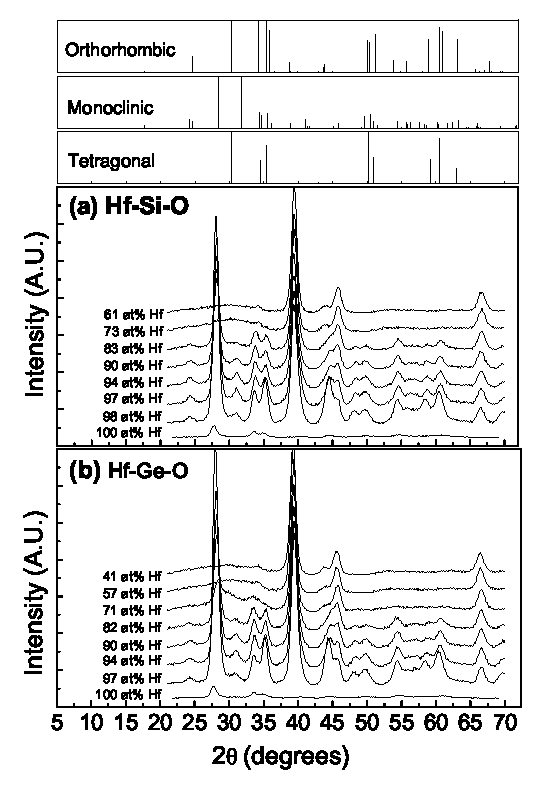
\includegraphics[width=0.5\linewidth]{chapter_6/hfsigeox_wpdf.eps}
\caption{The XRD spectra for (a) (HfO$_{2}$)$_{1-x}$(SiO$_{2}$)$_{x}$ and (b) (HfO$_{2}$)$_{1-x}$(GeO$_{2}$)$_{x}$ plotted for several different Hf cation compositions. The observed patterns between Si and Ge doped HfO$_{2}$ are highly similar, demonstrating their chemical resemblance. The diffraction pattern for the mixed films show that the monoclinic phase is the dominant phase, however comparison with available diffraction patterns suggest the presence of other metastable phases. For reference the diffraction pattern of pure HfO$_{2}$ is shown at the bottom. The weak reflections reveal the presence of partially crystalline domains.}  
\label{fig:xrd1}
\end{figure}

For the hafnium based systems a change in composition elicits a clear shift in the structure from amorphous (HfO$_{2}$ poor compositions) to polycrystalline (HfO$_{2}$ rich compositions), as seen in Figure \ref{fig:xrd1}. As a reference we also present the diffraction pattern of pure HfO$_{2}$ deposited under similar conditions. The pattern displays very weak reflections signifying the presence of small crystalline domains embedded in a mostly disordered matrix. 

It is not unusual that the doped hafnia films deposited at low temperatures show sign of crystallinity. Thicker HfO$_{2}$ films may crystallize \cite{Ritala1994} (our films are 100 - 300 nm thick) and deposition conditions \cite{Jones1992, Wang2008} play a role in whether HfO$_{2}$ becomes amorphous or crystalline. Even for films that seem to be amorphous HfO$_{2}$ thin films, careful inspection of its structure reveals that it exhibits a certain level of medium-range order, a characteristic of a fairly poor glass former. \cite{Ho2003} Crystallinity decreases with increasing substitution of glass formers SiO$_{2}$ and GeO$_{2}$ and is consistent with our intuition that substitution of glass formers should increase the crystallization temperature of the film. \cite{Maria2002}

A direct comparison of the diffraction patterns between the two systems shows an uncanny resemblance, demonstrating the chemical similarities between SiO$_{2}$ and GeO$_{2}$. Continuous rings are observed in the area detector pattern, which indicate that the grains are equiaxed with no preferential orientation. Comparison with powder diffraction and calculated diffraction patterns retrieved from the Inorganic Crystal Structure Database (ICSD) with the integrated powder diffraction patterns show that the HfO$_{2}$ rich crystalline films primarily consist of the monoclinic phase, indicated definitively by the peak at 28.2$^{\circ}$. Note, the bulk equilibrium phase of HfO$_{2}$ at room temperature is monoclinic. 

\begin{figure}
\centering
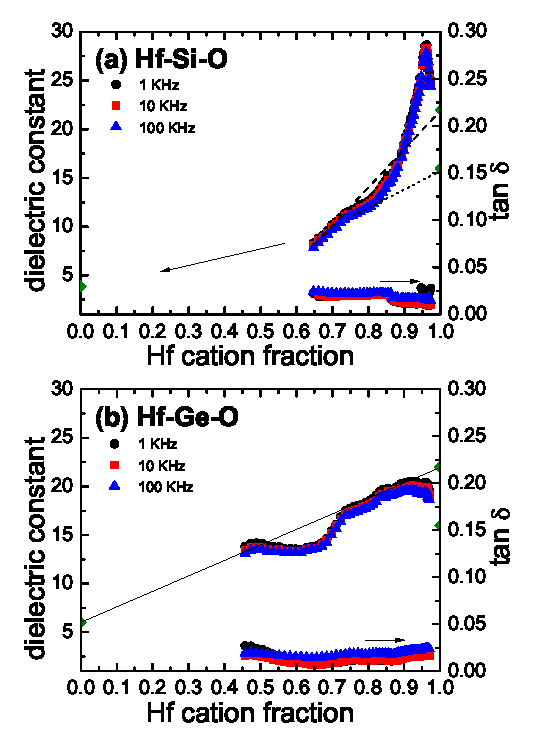
\includegraphics[width=0.5\linewidth]{chapter_6/eps_hfsigeox.eps}
\caption{The dielectric constant and dissipation factor of (a) (HfO$_{2}$)$_{1-x}$(SiO$_{2}$)$_{x}$ and (b) (HfO$_{2}$)$_{1-x}$(GeO$_{2}$)$_{x}$ as function of Hf cation composition. In contrast to the XRD patterns in Figure \ref{fig:xrd1}, the dielectric behavior of the two materials are different.}
\label{fig:eps1}
\end{figure} 

However, we see the peaks are not well aligned with a pure monoclinic phase. The structural deviation is reflected in the dielectric behavior of the two systems as a function of composition (Figure \ref{fig:eps1}). For (HfO$_{2}$)$_{1-x}$(SiO$_{2}$)$_{x}$, we see that a rough extrapolation of $\varepsilon_{r}$ to pure SiO$_{2}$ in the amorphous region ($65 < \text{at\% Hf} < 75$) points to about 3.9. A linear extrapolation in the other direction to pure HfO$_{2}$ (denoted by the dashed line) yields $\varepsilon_{r}$ of 22, the dielectric constant of pure amorphous HfO$_{2}$. \cite{Ceresoli2006} At the onset of crystallization in the region $75 < \text{at\% Hf} < 85$, we observe a slope change in $\varepsilon_{r}$ (dotted line) such that now $\varepsilon_{r}$ extrapolates to the dielectric constant of monoclinic HfO$_{2}$, $\varepsilon_{r} = 16$. \cite{Zhao2002} Further addition of HfO$_{2}$ causes another slope change at $\sim$85 at\% Hf accompanied by a discontinuity in tan $\delta$. In this region $\varepsilon_{r}$ is enhanced dramatically to a maximum dielectric constant of approximately 28 at a concentration of 96 at\% Hf. The dielectric behavior in this region is clear indication that the monoclinic phase is not the sole phase within this composition range, since $\varepsilon_{r}$ of a pure monoclinic phase is only 16. Finally, the dielectric constant drops down for even higher Hf concentrations.

The dielectric behavior of (HfO$_{2}$)$_{1-x}$(GeO$_{ 2}$)$_{x}$ is clearly different from (HfO$_{2}$)$_{1-x}$(SiO$_{ 2}$)$_{x}$, even though their diffraction patterns are highly similar. At 50 $  \text{at\% Hf}$, the dielectric constant is consistent with the linear interpolation (solid line), between the endmember values for pure amorphous HfO$_{2}$ and GeO$_{2}$. Addition of Hf does not increase the dielectric constant and consequently, $\varepsilon_{r}$ is suppressed below the linear interpolation for $50 < \text{at\% Hf} < 70$. At the onset of crystallization ($\sim$70 at\% Hf) the dielectric constant once again becomes collinear to the linear interpolation. Increasing the Hf concentration further does not result in any kind of enhancement; the dielectric constant of the Hf richest composition is 19, roughly between the amorphous and monoclinic dielectric constant. 

Without further analysis, it is difficult to determine the cause for the trends seen in Figure \ref{fig:eps1}. Nevertheless, the enhancement of $\varepsilon_{r}$ observed in (HfO$_{2}$)$_{1-x}$(SiO$_{ 2}$)$_{x}$ is unfeasible without a stabilization of high $\varepsilon_{r}$ phases such as the tetragonal, or cubic like phase. It has been shown that both Si and Ge are effective stabilizers of the tetragonal phase, where Si is slightly more effective than Ge, i.e. lower concentrations of the dopant is required. \cite{Fischer2008a, Tomida2006} Its effectiveness in part may be attributed to ionic radii where smaller dopants such as Si and Ge tend to stabilize the tetragonal phase. \cite{Lee2008} For stabilization of the tetragonal phase, calculations by Lee et al. \cite{Lee2008}  predict a minimum concentration of 10.9\% for Si and 18.6 \% for Ge. Furthermore, when considering temperature as a parameter,  Debernardi predicts that at 320 K, 12.5\% Ge is required to stabilize the tetragonal phase. \cite{Debernardi2012} Our data suggests that it is fairly easy to stabilize a tetragonal-like phase when Si is the dopant, while Ge seems less effective and may require additional processing. Deviations from predicted values may be caused by stress and grain size effects, which shift the transformation temperature. \cite{Garvie1978} It is possible that the deposition process and the dopant in combination have created stresses in the film causing the variations.

\begin{figure}
\centering
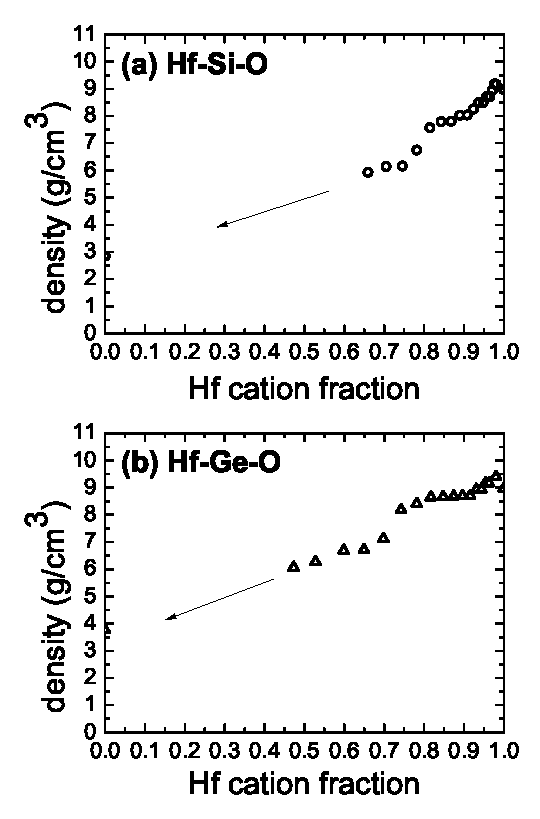
\includegraphics[width=0.5\linewidth]{chapter_6/hfsiox_density.eps}
\caption{The density of (a) (HfO$_{2}$)$_{1-x}$(SiO$_{2}$)$_{x}$ and (b) (HfO$_{2}$)$_{1-x}$(GeO$_{2}$)$_{x}$ as function of Hf cation composition determined using XRR. Crystallization of the film causes the film density to jump dramatically.}
\label{fig:hfd1}
\end{figure}

\begin{figure}
\centering
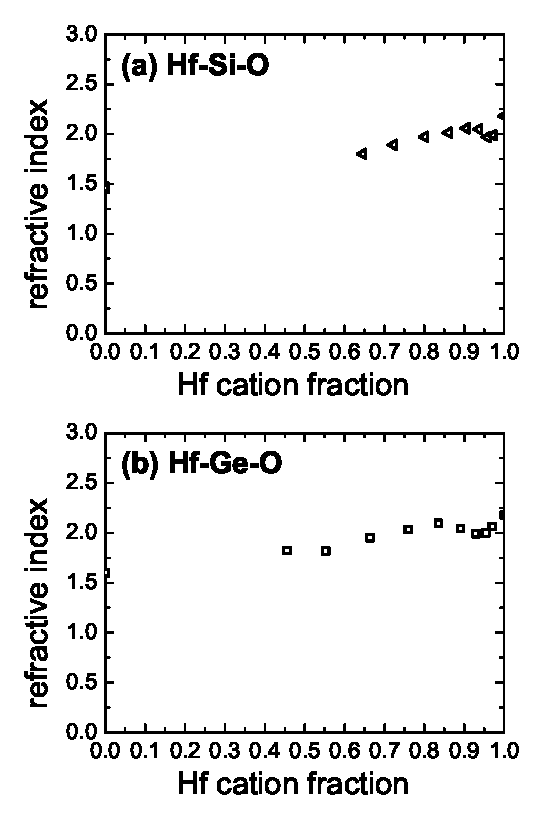
\includegraphics[width=0.5\linewidth]{chapter_6/n_hfsigeox.eps}
\caption{Refractive index of (a) (HfO$_{2}$)$_{1-x}$(SiO$_{2}$)$_{x}$ and (b) (HfO$_{2}$)$_{1-x}$(GeO$_{2}$)$_{x}$ as function of Hf cation composition.}
\label{fig:hfn1}
\end{figure}

We also present the density and the refractive indices in Figures \ref{fig:hfd1} and \ref{fig:hfn1} respectively as a function of Hf composition. The density for both systems increases linearly with increasing Hf composition in the amorphous regions. Crystallization of the film is marked by a clear jump in the density. The onset of crystallinity for (HfO$_{2}$)$_{1-x}$(GeO$_{2}$)$_{x}$ is slightly lower in composition in comparison to the (HfO$_{2}$)$_{1-x}$(SiO$_{2}$)$_{x}$; approximately 70 at\% Hf for Ge doped HfO$_{2}$ versus 80 at\% Hf for Si doping. This suggests the slightly higher effectiveness of SiO$_{2}$ as a glass former compared to GeO$_{2}$. We find that although there is a general correlation between increased density  and dielectric constant, there is no direct evidence which explains the large disparity in dielectric behavior between (HfO$_{2}$)$_{1-x}$(SiO$_{2}$)$_{x}$ and (HfO$_{2}$)$_{1-x}$(GeO$_{2}$)$_{x}$. For example, direct comparison of the density of both systems at around 96 at\% Hf, the density of (HfO$_{2}$)$_{1-x}$(SiO$_{2}$)$_{x}$ is 8.72 g/cm$^{3}$, whereas the density of (HfO$_{2}$)$_{1-x}$(GeO$_{2}$)$_{x}$ is 9.17 g/cm$^{3}$. This in turn implies that substantial differences in the phononic contributions may be at play.   

The refractive index varies linearly with Hf composition for both systems. For the Hf richest compositions a slight depression from a linear trend is observed. A large variation in the refractive index for HfO$_{2}$ is not uncommon, \cite{Jones1992} but a more likely contribution is the increase in roughness with crystallinity, \cite{Ritala1994} indicated by a larger mean squared error (MSE) in the fitting, as our simple model does not take into account surface roughness.  	
\subsection{(Nb$_{2}$O$_{5}$)$_{1-x}$(GeO$_{2}$)$_{x}$ and  (Ta$_{2}$O$_{5}$)$_{1-x}$(SnO$_{2}$)$_{x}$}

The XRD patterns for (Nb$_{2}$O$_{5}$)$_{1-x}$(GeO$_{2}$)$_{x}$ and  (Ta$_{2}$O$_{5}$)$_{1-x}$(SnO$_{2}$)$_{x}$ are shown in Figure \ref{fig:xrd2}. Patterns for (Nb$_{2}$O$_{5}$)$_{1-x}$(GeO$_{2}$)$_{x}$ show that it is amorphous for all compositions investigated, whereas crystallization is observed for tantalum poor compositions in (Ta$_{2}$O$_{5}$)$_{1-x}$(SnO$_{2}$)$_{x}$. Comparison with Power Diffraction File (PDF) suggest that the peaks embody the symmetry of the tetragonal (cassiterite) phase.

\begin{figure}
\centering
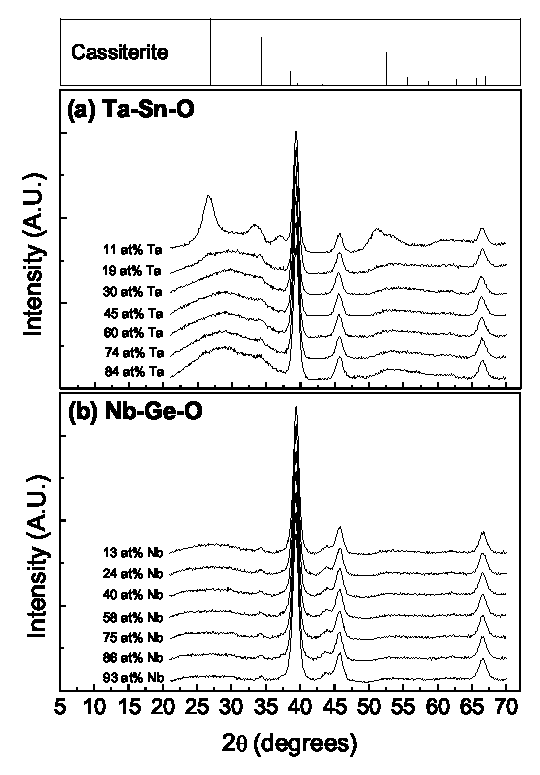
\includegraphics[width=0.5\linewidth]{chapter_6/tanbsngeox_wpdf.eps}
\caption{XRD spectra for (a) (Nb$_{2}$O$_{5}$)$_{1-x}$(GeO$_{2}$)$_{x}$ and (b) (Ta$_{2}$O$_{5}$)$_{1-x}$(SnO$_{2}$)$_{x}$ plotted for several cation compositions. The lack of any discernible diffraction peaks indicate that the (Nb$_{2}$O$_{5}$)$_{1-x}$(GeO$_{2}$)$_{x}$ is x-ray amorphous for the entire composition range probed. (Ta$_{2}$O$_{5}$)$_{1-x}$(SnO$_{2}$)$_{x}$ is x-ray amorphous for high Ta$_{2}$O$_{5}$ rich composition, but crystallizes at high SnO$_{2}$ concentrations.}
\label{fig:xrd2}
\end{figure}

\begin{figure}
\centering
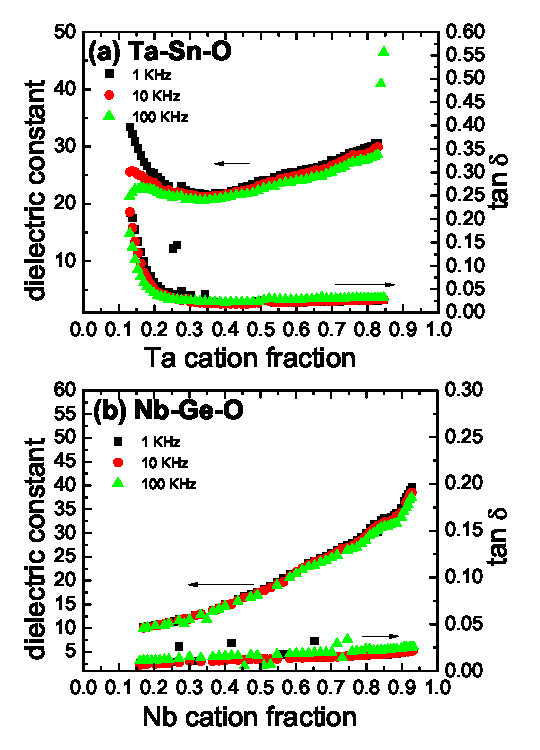
\includegraphics[width=0.5\linewidth]{chapter_6/eps_nbta.eps}
\caption{The dielectric constant and dissipation factor for (a) (Nb$_{2}$O$_{5}$)$_{1-x}$(GeO$_{2}$)$_{x}$ and (b) (Ta$_{2}$O$_{5}$)$_{1-x}$(SnO$_{2}$)$_{x}$ plotted as a function of composition. The  dielectric constant of (Nb$_{2}$O$_{5}$)$_{1-x}$(GeO$_{2}$)$_{x}$ shows a mostly linear dependence in $\varepsilon_{r}$ with composition, whereas (Ta$_{2}$O$_{5}$)$_{1-x}$(SnO$_{2}$)$_{x}$ shows a nondispersive and highly dispersive region.}
\label{fig:eps2}
\end{figure}

The sensitivity of the dopant concentration on the dielectric behavior of (Ta$_{2}$O$_{5}$)$_{1-x}$(SnO$_{2}$)$_{x}$ is shown in Figure \ref{fig:eps2}, where two distinct regions of dielectric behavior can be distinguished. For high Ta$_{2}$O$_{5}$ concentrations we observe a near linear dependence on the dielectric constant and in this region, the dissipation factor is also low ($\tan{\delta}<0.1$) indicating a high quality insulating film. Substitution of an aliovalent cation does not seem to promote a defect mediated transport mechanism such as hopping conductivity, as suggested by the low dissipation factor. Similarly, the substitution of ZrO$_{2}$ in Ta$_{2}$O$_{5}$ decreases the conductivity of Ta$_{2}$O$_{5}$ phase, the opposite of what is expected for a classical point defect model. \cite{Bredesen1988} The dielectric constant of the most Ta$_{2}$O$_{5}$ rich composition is around 27 at approximately 85 at\% Ta. Linearly extrapolating to pure Ta yields a dielectric constant of approximately $\varepsilon_{r} = 31$ which is enhanced over that of pure amorphous Ta$_{2}$O$_{5}$ ($\varepsilon_{r} = 22$), \cite{Barron2009} while extrapolation to pure SnO$_{2}$ gives $\varepsilon_{r} = 13$, consistent with literature values. \cite{albers1972} With further incorporation of SnO$_{2}$ $\varepsilon_{r}$ becomes dispersive, evidenced by a high dissipation factor ($\tan{\delta}>0.1$) and the highly frequency dependent nature of $\varepsilon_{r}$. This is not surprising since SnO$_{2}$ is a conductive oxide. \cite{singh2008} Diffraction patterns (Figure \ref{fig:xrd2}) show that the onset of crystallization correlates with the dispersive behavior, hence the dispersive nature of the film is likely caused by conduction within the SnO$_{2}$ rather than defects in Ta$_{2}$O$_{5}$. 

The dielectric constant of amorphous (Nb$_{2}$O$_{5}$)$_{1-x}$(GeO$_{2}$)$_{x}$ scales linearly with composition, with low dissipation factors, and shows no sign of dispersive behavior (Figure \ref{fig:eps2}). At an Nb cation concentration of 93\%  $\varepsilon_{r} \sim 42.5$, while extrapolation of $\varepsilon_{r}$ to pure Nb$_{2}$O$_{5}$ indicates a $\varepsilon_{r}$ for pure Nb$_{2}$O$_{5}$ $\sim 47-48$, which is comparable with $\varepsilon_{r}$ of fully oxidized Nb$_{2}$O$_{5}$ ($\varepsilon_{r}= 45-50$). \cite{Kukli1999,Pignolet1995}
Though the dielectric constant may not be dramatically enhanced over the end member, an insulating amorphous Nb$_{2}$O$_{5}$ thin film oxide may still be of technological interest, 
in particular since it is a  conductive oxide, \cite{Greener1961} that is sensitive to oxygen partial pressure during deposition. \cite{Pignolet1995} Because conductivity in Nb$_{2}$O$_{5}$ is inversely related to oxygen partial pressure it is often attributed to oxygen ion vacancies in Nb$_{2}$O$_{5}$  creating charge carriers that are thermally excited into  the conduction band. \cite{Greener1961} Doping aliovalent cations often create sites that enable dielectric relaxation via hopping. For instance, previous measurements on sintered (Nb$_{2}$O$_{5}$)$_{0.92}$(SiO$_{2}$)$_{0.08}$ bulk ceramic samples exhibited significant frequency dependent dielectric relaxation at room temperature. \cite{Choosuwan2003} Three distinct mechanisms were identified and the authors hypothesized that the relaxation species composed of hopping ions between the Nb and the substituted Si ion and the large dispersion is accompanied by a substantially higher dielectric constant ($\varepsilon_{r}\approx 125$ at room temperature). \cite{Choosuwan2003} 

\begin{figure}
\centering
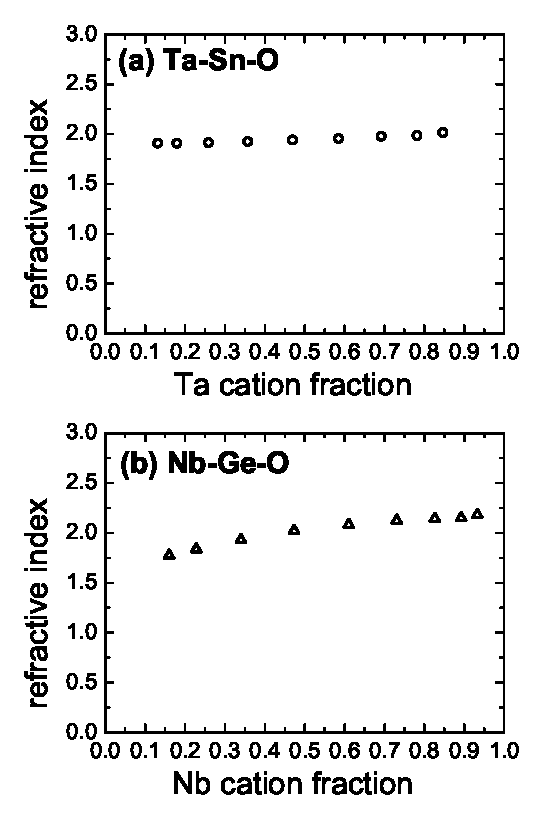
\includegraphics[width=0.5\linewidth]{chapter_6/n_tanb.eps}
\caption{Refractive index of (a) (Nb$_{2}$O$_{5}$)$_{1-x}$(GeO$_{2}$)$_{x}$ and (b) (Ta$_{2}$O$_{5}$)$_{1-x}$(SnO$_{2}$)$_{x}$ as function of Hf cation composition.}
\label{fig:ntanb}
\end{figure}

\begin{figure}
\centering
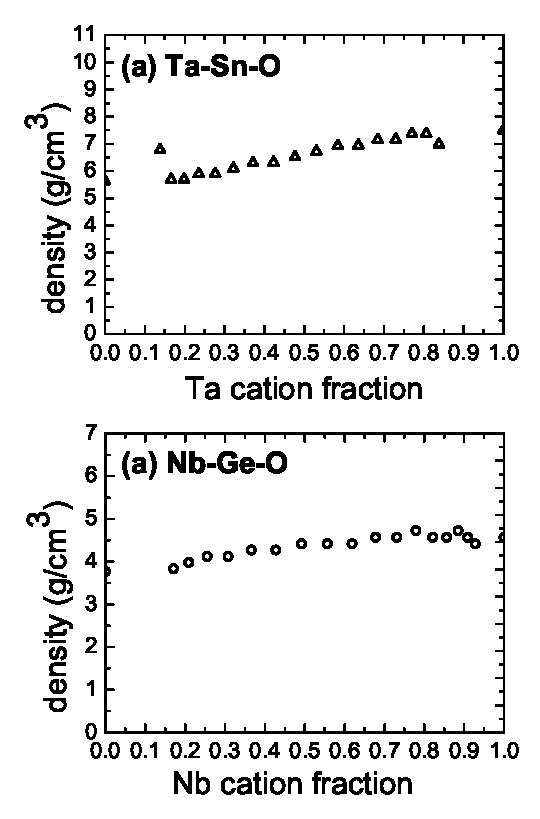
\includegraphics[width=0.5\linewidth]{chapter_6/tanbox_density.eps}
\caption{The density of (a) (Nb$_{2}$O$_{5}$)$_{1-x}$(GeO$_{2}$)$_{x}$ and (b) (Ta$_{2}$O$_{5}$)$_{1-x}$(SnO$_{2}$)$_{x}$ as function of Hf cation composition determined using XRR. The linear variation in density for (Nb$_{2}$O$_{5}$)$_{1-x}$(GeO$_{2}$)$_{x}$ as a function of composition reflects the amorphous nature of for all composition. (Ta$_{2}$O$_{5}$)$_{1-x}$(SnO$_{2}$)$_{x}$ densities also vary linearly except for the point where the film crystallizes.}
\label{fig:tanbden}
\end{figure}

Even with the introduction of GeO$_{2}$ into Nb$_{2}$O$_{5}$, the thin films exhibit low dissipation factors indicating the absence of a deleterious relaxation mechanism. Nonetheless, direct comparisons are difficult to make since the (Nb$_{2}$O$_{5}$)$_{0.92}$(SiO$_{2}$)$_{0.08}$ was a bulk crystalline ceramic, whereas our materials were amorphous thin films. Bulk crystalline ceramics contain grains and grain boundaries, which can contribute to several types of conduction mechanisms, which are absent in amorphous materials. 
     
Anomalous behaviors were not observed for the refractive indices for both systems (Figure \ref{fig:ntanb}) and the refractive index scales with composition. This trend is also reflected in the densities calculated from x-ray reflectivity (Figure \ref{fig:tanbden}). The density of the endmember values were also calculated directly from pure films deposited on to Si. Crystallization of the (Ta$_{2}$O$_{5}$)$_{1-x}$(SnO$_{2}$)$_{x}$ film at 0.14 Ta cation fraction causes the film density to jump to 6.78 g/cm$^{3}$ and is consistent with diffraction patterns and dielectric measurements. This makes it appear that the density is nonlinear, however the density of pure amorphous SnO$_{2}$ as seen in Figure \ref{fig:tanbden} is 5.62 g/cm$^{3}$ and is consistent with the linear trend. Since the refractive index reflects the electron density of the material increase in density should cause the refractive index to rise. Our refractive index measurements for (Ta$_{2}$O$_{5}$)$_{1-x}$(SnO$_{2}$)$_{x}$ do not go low enough in Ta cation fraction and thus we were not able to observe an increase in the refractive index. 

\section{Conclusion}

Using off-axis rf sputtering, we have studied the physical and dielectric properties of four pseudo-ternary oxides of varying composition: (HfO$_{2}$)$_{1-x}$(SiO$_{2}$)$_{x}$, (HfO$_{2}$)$_{1-x}$(GeO$_{2}$)$_{x}$, (Nb$_{2}$O$_{5}$)$_{1-x}$(GeO$_{2}$)$_{x}$, and (Ta$_{2}$O$_{5}$)$_{1-x}$(SnO$_{2}$)$_{x}$. Both (HfO$_{2}$)$_{1-x}$(SiO$_{2}$)$_{x}$ and (HfO$_{2}$)$_{1-x}$(GeO$_{2}$)$_{x}$ crystallized with increasing HfO$_{2}$ compositions and became amorphous with increasing concentrations of Si(Ge)O$_{2}$. The diffraction patterns of the two systems were similar, but the dielectric constants varied differently with composition. A clear peak in the dielectric constant can be observed in the (HfO$_{2}$)$_{1-x}$(SiO$_{2}$)$_{x}$ films, with a maximum dielectric constant of $\varepsilon_{r} = 28$ at 96 at$\%$ Hf, while the dielectric constant of (HfO$_{2}$)$_{1-x}$(GeO$_{2}$)$_{x}$ plateaus around $\varepsilon_{r} = 19$. Reflectivity measurements were consistent with the diffraction measurements and provided further detail into the amorphous-crystalline phase transition. The onset of crystallinity is slightly higher for the SiO$_{2}$ doped films; 80 at$\%$ Hf versus 70 at$\%$ for the GeO$_{2}$ doped films. In contrast to the dielectric constants, the refractive indices varies roughly linearly with composition.

(Ta$_{2}$O$_{5}$)$_{1-x}$(SnO$_{2}$)$_{x}$ was amorphous for SnO$_{2}$ poor compositions and crystallized into the cassiterite phase only for the most SnO$_{2}$ rich composition evaluated, and is indicated by a sudden increase in density. Increased dielectric dispersion and dissipation factor with increasing SnO$_{2}$ suggest that the film is becomes more conductive, where conduction is most likely through polycrystalline SnO$_{2}$ grains. Finally, (Nb$_{2}$O$_{5}$)$_{1-x}$(GeO$_{2}$)$_{x}$ was amorphous for all measured compositions and showed no anomalous features in the dielectric constant and refractive index. Not surprisingly, the density of the solid-solution changes linearly with composition. Doping low levels of GeO$_{2}$ into Nb$_{2}$O$_{5}$ resulted in a high quality dielectric and may be useful for applications requiring a high dielectric constant oxides.

% probably needs to be updated %
\section{Acknowledgments}
This work was supported by the U.S. Department of Energy under Grant No. DE-FG02-06ER06-15. This work was performed in part at the Cornell NanoScale Facility, a member of the National Nanotechnology Infrastructure Network, which is supported by the National Science Foundation under Grant No. ECS-0335765. Additionally, this work made use of the Cornell Center for Materials Research facilities with support from the National Science Foundation Materials Research Science and Engineering Center program under Grant No. DMR-0520404.



% chapter 7
\chapter{Summary and Future Outlook}

In this dissertation, we have evaluated the properties of various complex amorphous thin film oxides synthesized by combinatorial sputtering. We mostly focused on two aspects of materials science: structure and property. Structurally, amorphous materials are inherently hard to characterize and throughout this study, we learned that this is especially true for thin film amorphous materials. However, by combining several different techniques we were able to effectively characterize their structure at both the macroscopic and local level. Taking what we learned structurally and what we learned by probing their dielectric properties, we learned something about the structure-property relations of the complex amorphous oxides.  

In chapter 3, we found that the structural and dielectric properties of two chemically similar amorphous oxides, namely Ta-Ge-O and Ta-Si-O, were significantly different. We saw that the dielectric constant of Ta-Ge-O was dramatically enhanced over linear interpolation of its end members, while Ta-Si-O did not exhibit this behavior. This type of enhancement was not observed in the refractive index for both materials. We used x-ray reflectivity to directly probe the density of the thin films as a function of composition. This technique allowed us to calculate the polarizabilities of the oxides without relying on tabulated values, avoiding any additive assumptions of the individual polarizabilities. We also explored the limitations of the Clausius-Mossotti relation applied to the two systems and found that the use of tabulated atomic polarizabilities and experimentally inferred volumes systematically underestimates the dielectric constant in both systems. This result highlights the importance of directly calculating the densities and atomic polarizabilities. We then used FTIR to explore the changes in active phonon modes of Ta-Ge-O as a function of composition. The spectra did not show any obvious features in the frequency range that would explain the anomalous dielectric behavior of Ta-Ge-O. It is likely that the phonon modes contributing to the enhancement exist at lower wavenumbers. Therefore, it might be worthwhile to conduct a careful far-infrared spectroscopy experiment to cover the sub 400 cm$^{-1}$ range in future studies. A Raman spectroscopy study may also be a good complement to FTIR. 

In chapter 4, we extended the study in chapter 3 by probing the atomic structure of pure Ta$_{2}$O$_{5}$ and Ta-Ge-O using high energy synchrotron x-ray diffraction and absorption methods. Simultaneously applying different techniques greatly reduced the uncertainty in structure space by constraining the possible structural parameters of the local environment. To reduce scattering from the substrate, we sputtered the thin films on silicon nitride windows. We found bond lengths and coordination numbers of amorphous Ta$_{2}$O$_{5}$ to be similar to values reported in previous studies, where the Ta-O coordination was found to be lower than those measured in crystalline Ta$_{2}$O$_{5}$ compounds. Past research suggests this is due to 1) Ta-O having a fairly low field strength (for example compared Si-O which is a good network former) 2) the Ta cation is large in size. 

Doping of GeO$_{2}$ in Ta$_{2}$O$_{5}$ result in substantial changes to the local environment. We identify two distinct regions in composition based on pair bond distance and coordination data. The Ta-O/Ge-O bond distance does not differ greatly from pure Ta$_{2}$O$_{5}$ for high Ta cation fractions; only when a considerable amount of GeO$_{2}$ is added does $r_{Ta-O/Ge-O}$ begin to decrease to $r_{Ge-O}$. Our EXAFS data also shows that the Ta-O structural unit experiences an anisotropic distortion due to Ge doping. We find that the most dramatic change in the local environment around Ta occurs for the metal-metal (M-M) pairs, namely Ta-Ta and Ta-Ge. Further, the trend in the O-O pair bond distance was explained as a consequence of a high Ta-Ge coordination at fairly low GeO$_{2}$ composition. When the composition of Ta and Ge cations are roughly equal, the short-range order starts to resemble that of low temperature crystalline Ta$_{2}$O$_{5}$, evidenced by the coordination number of the Ta-O inner shell. Moreover, we surmise that a major factor in the reduction of density observed in chapter 3 is due to the change in coordination of inner M-M pairs, while there is only minimal contribution from changes in M-O and M-M bond distances. This suggests that network conformation has a larger effect on the density than simple changes in bond length. \textbf{need to write a little more here}

In chapter 5, we studied the composition dependence of the dielectric properties of another complementary system, Zr-Al-O and Zr-Si-O. Specifically, we used these two systems to systematically investigate the effect of the presence or absence of crystallinity on the dielectric constant and breakdown field. An essentially linear variation of the static dielectric constant, $\varepsilon_s$, was observed as a function of composition, $x$, for compositions rich in the p-block element, i.e., $x>0.4$, for both chemical systems. However an abrupt change in $\varepsilon_s$ is found near $x \approx 0.35$, associated with the onset of crystallinity in as-deposited films. 
Measurements of the index of refraction at optical frequencies, combined with a simple Clausius-Mossotti interpretation, indicates that low-frequency (ionic) contributions to the polarizability exhibit systematic deviation with respect to values linearly interpolated from the endmembers. These trends are not consistently affected by the presence of crystalline order, but are related to changes associated with heterogeneous local oxygen coordination and bonding. There were no significant differences in the breakdown field associated with the level of crystallinity in both systems.

In chapter 6, we expand on the study in chapter 3 by substituting different cations in the Ta/Ge cation site which include the combinations Hf-Si-O, Hf-Ge-O, Ta-Sn-O, and Nb-Ge-O. Hf-Si-O and Hf-Ge-O showed similar trends in the x-ray diffraction spectra as a function of composition. Both remain amorphous until a critical Hf cation concentration is reached, upon which crystallizing into a mostly monoclinic phase mixed with possibly tetragonal and orthorhombic phases. Crystallization of the oxides were clearly reflected in the density measurements as jumps in the density for both systems. However, when we probed the dielectric constant of each system as a function composition, the two systems show dissimilar trends in $\varepsilon_{r}$, namely Hf-Si-O shows an enhanced $\varepsilon_{r}$ of approximately 28 at a concentration of 96 at\% Hf, while $\varepsilon_{r}$ for Hf-Ge-O is not enhanced for any composition. The dielectric enhancement observed for Hf-Si-O is clear indication that the monoclinic phase is not the sole phase within this composition range, since $\varepsilon_{r}$ of a pure monoclinic phase is only 16. The refractive index is linear with composition for both Hf-Si-O and Hf-Ge-O.

Ta-Sn-O and Nb-Ge-O are quite different structurally and electronically compared to Hf-Si-O and Hf-Ge-O. Inspection of the diffraction spectra indicates that both systems remain amorphous for most of the compositions probed in the study. The exception is for the Sn rich region in Ta-Sn-O ($<$ 30 at\% Ta), where SnO$_{2}$ crystallizes into a tetragonal (cassiterite) phase. Crystallization of SnO$_{2}$ is clearly reflected in the dielectric constant below 30 at\% Ta by two measures: the increased dispersion in the dielectric factor and the marked increase in dissipation factor. For compositions $>$ 30 at\% Ta, Ta-Sn-O remains amorphous for all compositions investigated ($\sim$ 15 at\% Ta $<$ x $<$ $\sim$85 at\% Ta). Nb-Ge-O is x-ray amorphous for $\sim$15 at\% Ta $<$ x $<$ $\sim$ 95 at\% Ta, thus not surprisingly, the dielectric constant and the refractive index scales linearly with composition. It is interesting to note that the dielectric constant in the Nb rich side does not become dispersive since pure Nb$_{2}$O$_{5}$ films are generally conducting. For a more detailed analysis of the dielectric behavior of the oxide, it may be worthwhile to investigate the relaxation mechanism of the oxide as a function of frequency. The density of Ta-Sn-O and Nb-Ge-O varies linearly with composition with the exception of the jump in density for Ta-Sn-O, where SnO$_{2}$ crystallizes.                

There are several different paths we can go down from here. An obvious choice would be to probe the local environment around Ge in Ta-Ge-O using EXAFS. Another low hanging fruit would be to use high energy x-ray diffraction and absorption methods to study Ta-Si-O. Stuctural measurements can be complimented with infrared spectroscopy to directly observe the changes in phonon modes as a function of Ta cation composition for Ta-Ge-O and Ta-Si-O, to establish a more rigorous structure-property relationship. Obviously we are not limited to Ta based systems; we can apply our composition spread approach to rapidly analyze the local structure variation of several different amorphous systems, including ternary oxides. Finally, we can utilize these materials in novel device applications to study changes in device performance with composition. For example, it would be interesting to study the effects of composition in resisitive memory and logic devices such as memristors.


\bibliography{thesis}
\end{document}
